\documentclass{article}
\usepackage[utf8]{inputenc}
\usepackage{authblk}
\usepackage{setspace}
\usepackage[margin=1.25in]{geometry}
\usepackage{graphicx}
% \graphicspath{ {./figures/} }
\graphicspath{ {../figures/} }
\usepackage{subcaption}
\usepackage{amsmath}
\usepackage{lineno}
\linenumbers

\usepackage{enumerate}
\DeclareMathOperator{\diag}{diag}
\usepackage{multirow}
\usepackage{booktabs}
\usepackage{footnote}
\usepackage{bm}
\usepackage[ruled,linesnumbered]{algorithm2e}
\setcounter{MaxMatrixCols}{20}
\usepackage{tikz}
\usetikzlibrary{arrows.meta, calc, fit, positioning, quotes, graphs, shapes.geometric}
\def\T{\mathrm{T}}

%%%%%% Bibliography %%%%%%
% Replace "sample" in the \addbibresource line below with the name of your .bib file.
\usepackage[style=nejm, 
citestyle=numeric-comp, 
sorting=none]{biblatex}
\addbibresource{ref.bib}

%%%%%% Title %%%%%%
% Full titles can be a maximum of 100 characters, including spaces. 
% Title Format: Use title case, capitalizing the first letter of each word, except for certain small words, such as articles and short prepositions
% \title{Using a Directed Graph Model and Greedy Algorithm to Determine the Maximum Allowable Current in a Reconfigurable Battery System}
\title{Maximum Allowable Current Determination of RBS By Using a Directed Graph Model and Greedy Algorithm}

%%%%%% Authors %%%%%%
% Authors should be listed in order of contribution to the paper, by first name, then middle initial (if any), followed by last name.
% Authors should be listed in the order in which they will appear in the published version if the manuscript is accepted. 
% Use an asterisk (*) to identify the corresponding author, and be sure to include that person’s e-mail address. Use symbols (in this order: †, ‡, §, ||, ¶, #, ††, ‡‡, etc.) for author notes, such as present addresses, “These authors contributed equally to this work” notations, and similar information.
% You can include group authors, but please include a list of the actual authors (the group members) in the Supplementary Materials.
\author[1$\dag$]{Binghui Xu}
\author[1$\dag$]{Guangbin Hua}
\author[1*]{Cheng Qian}
\author[1,2]{Quan Xia}
\author[1]{Bo Sun}
\author[1]{Yi Ren}
\author[1]{Zili Wang}

%%%%%% Affiliations %%%%%%
\affil[1]{School of Reliability and Systems Engineering, Beihang University, Beijing, 100191, China}
\affil[2]{School of Aeronautic Science and Engineering at Beihang University, Beijing, China}
\affil[*]{Address correspondence to: cqian@buaa.edu.cn}
\affil[$\dag$]{These authors contributed equally to this work.}

%%%%%% Date %%%%%%
% Date is optional
\date{}

%%%%%% Spacing %%%%%%
% Use paragraph spacing of 1.5 or 2 (for double spacing, use command \doublespacing)
\onehalfspacing

\begin{document}

\maketitle

%%%%%% Abstract %%%%%%
\begin{abstract}
Reconfigurable battery systems (RBSs) present a promising alternative to traditional battery systems due to their flexible and dynamically changeable topological structure that can be adapted to different battery charging and discharging strategies.
During RBS operation, a critical system parameter known as the maximum allowable current (MAC) become pivotal. This parameter is instrumental in maintaining the current of each individual battery within a safe range and serves as a guiding indicator for the system's reconfiguration, thereby ensuring its safety and reliability.
This paper proposes a method to calculate the MAC of arbitrary RBSs using a greedy algorithm in conjunction with a directed graph model of the RBS.
By introducing the shortest path of the battery, the greedy algorithm transforms the enumeration of switch states in the brute-force algorithm into the combination of the shortest paths, which greatly increases the efficiency with which the MAC is determined.
The directed graph model, based on the equivalent circuit, provides a specific method for calculating the MAC of a given structure.
The proposed method is validated on two published four-battery-RBSs and one with a more complex structure.
The results are the same as those of the brute-force algorithm, but the proposed method significantly improves the computational efficiency ($N_s 2^{N_s - N_b} \log_{10} N_b$ times faster than the brute force algorithm for an RBS with $N_b$ batteries and $N_s$ switches, theoretically).
The main advantage of the proposed method is its ability to calculate the MAC of RBSs with arbitrary structures, even in scenarios with random isolated batteries.
\end{abstract}

%%%%%% Main Text %%%%%%

\section{Introduction}

Battery energy storage systems (BESSs) are extensively used in various applications \cite{yangBatteryEnergyStorage2018}, such as wind power plants \cite{desiqueiraControlStrategySmooth2021} and space power systems \cite{schwanbeckInternationalSpaceStation2019,zhangDevelopmentProspectChinese2021}, to store and release high-quality electrical energy \cite{choCommercialResearchBattery2015}.
Typically, a BESS consists of numerous batteries interconnected by series-parallel circuitry to provide the required capacity storage.
However, traditional BESSs, in which the batteries are connected in a fixed topology, suffer from a significant weakness in their worst battery due to the so-called cask effect.
Moreover, if the worst battery fails during operation, it is highly likely to exacerbate the degradation of the other batteries, leading to reliability and safety issues \cite{yangUnbalancedDischargingAging2016,fengPropagationMechanismsDiagnosis2019,jeevarajanBatterySafetyQualifications2012}.
These problems have become significant technical barriers in many engineering projects requiring high reliability, such as developing new-generation space vehicles \cite{pomboHybridPowerSystem2021}. 


Reconfigurable battery systems (RBSs), which can dynamically switch as required to different circuit topologies, are expected to solve this problem \cite{hanNextGenerationBatteryManagement2020a}.
The switching circuit helps to isolate unhealthy batteries, thereby improving the safety and reliability of the battery system.
To illustrate the working principle of an RBS, we consider a typical RBS structure developed by Visairo \cite{visairoReconfigurableBatteryPack2008} (Fig. \ref{fig:stru-Visairo}), which is taken as an example to show the reconfiguration process.
In this structure, the batteries can be connected not only in series when the switches $S_1$, $S_5$, $S_6$, $S_7$, $S_8$, $S_9$, and $S_{13}$ are closed (see Fig. \ref{fig:stru-Visairo-serial}) but also in parallel when $S_1$, $S_2$, $S_3$, $S_4$, $S_5$, $S_9$, $S_{10}$, $S_{11}$, $S_{12}$, and $S_{13}$ are closed (Fig. \ref{fig:stru-Visairo-parallel}).
Furthermore, when an unhealthy battery, for instance, the orange one $B_3$ in Fig. \ref{fig:stru-Visairo-isolate}, appears in the RBS, it can be isolated by opening its two adjacent switches (i.e., $S_4$ and $S_{11}$), ensuring that the system remains in a reliable working mode.

\begin{figure}[htbp]
    \centering
    \begin{subfigure}[b]{0.45\textwidth}
        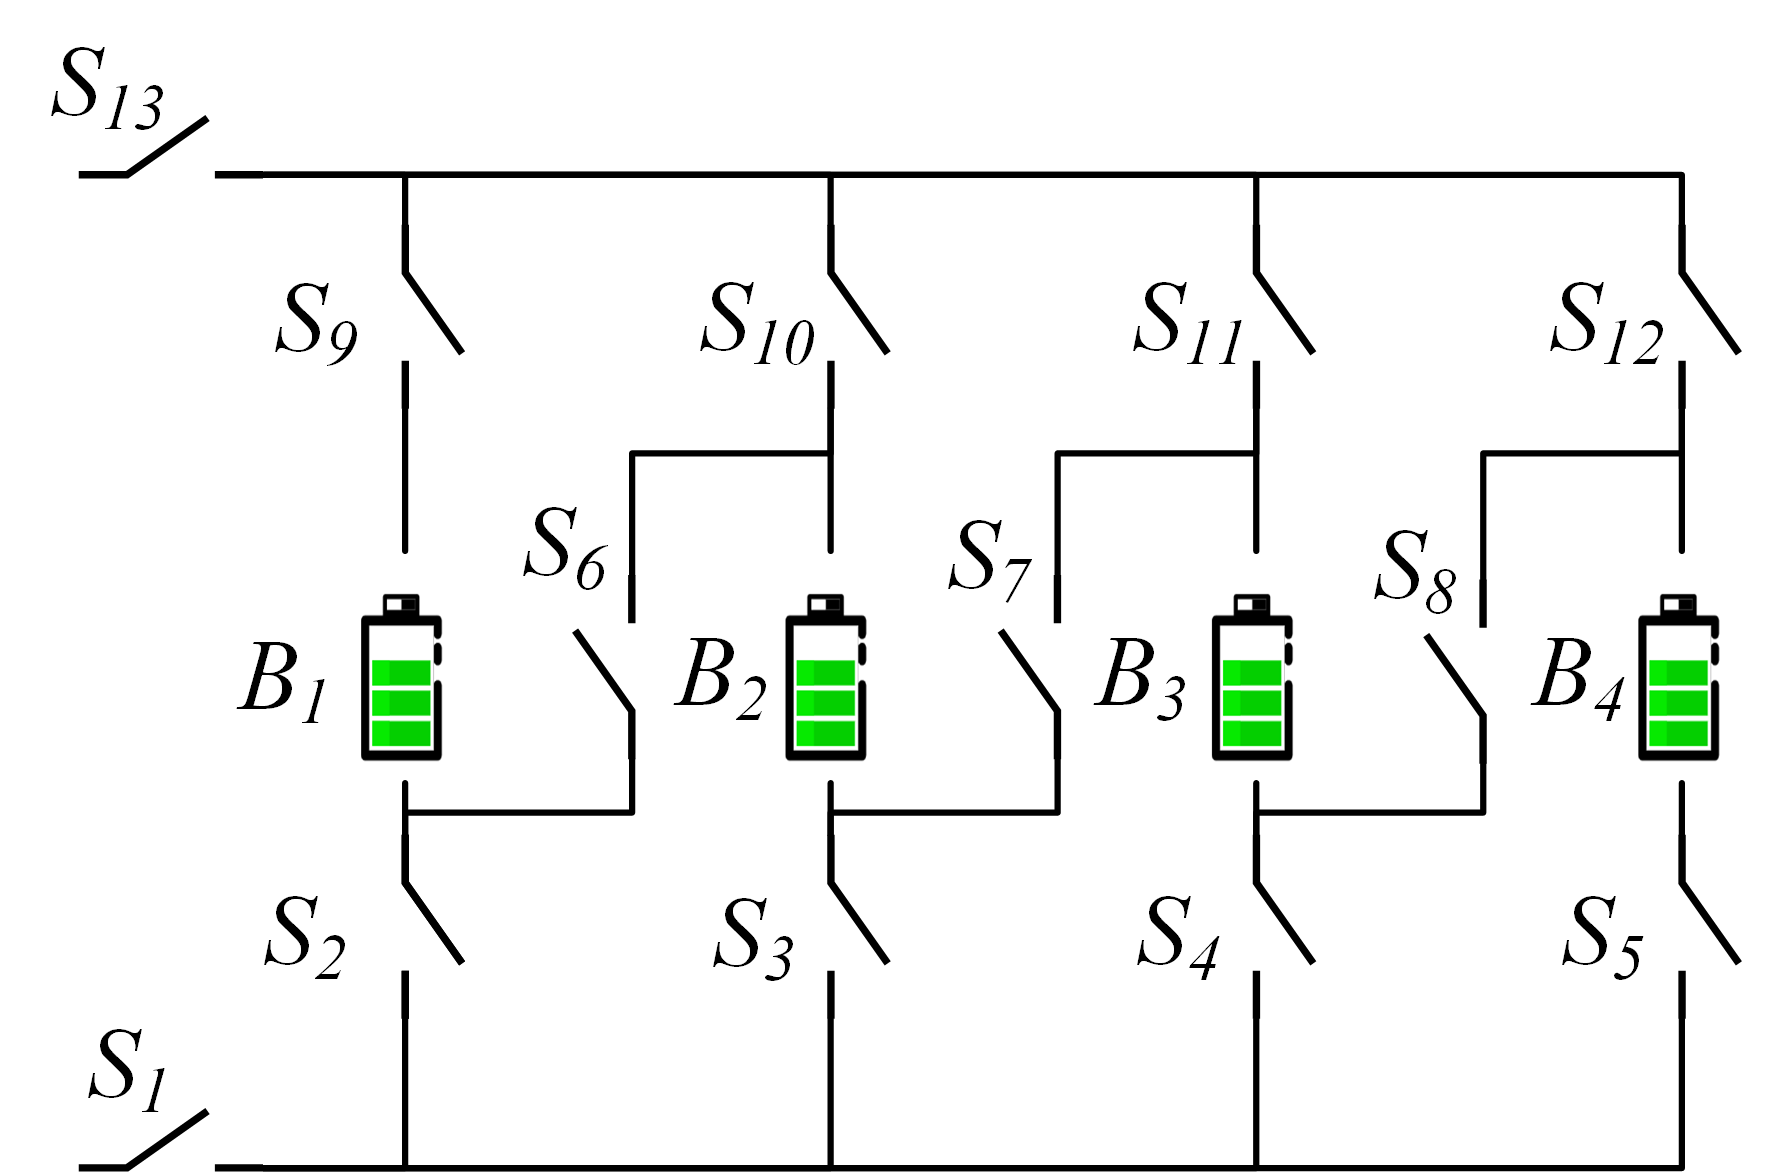
\includegraphics[width=\textwidth]{stru-V-origin.png}
        \caption{}
        \label{fig:stru-Visairo}
    \end{subfigure}
    \hspace{0.05\textwidth}
    \begin{subfigure}[b]{0.45\textwidth}
        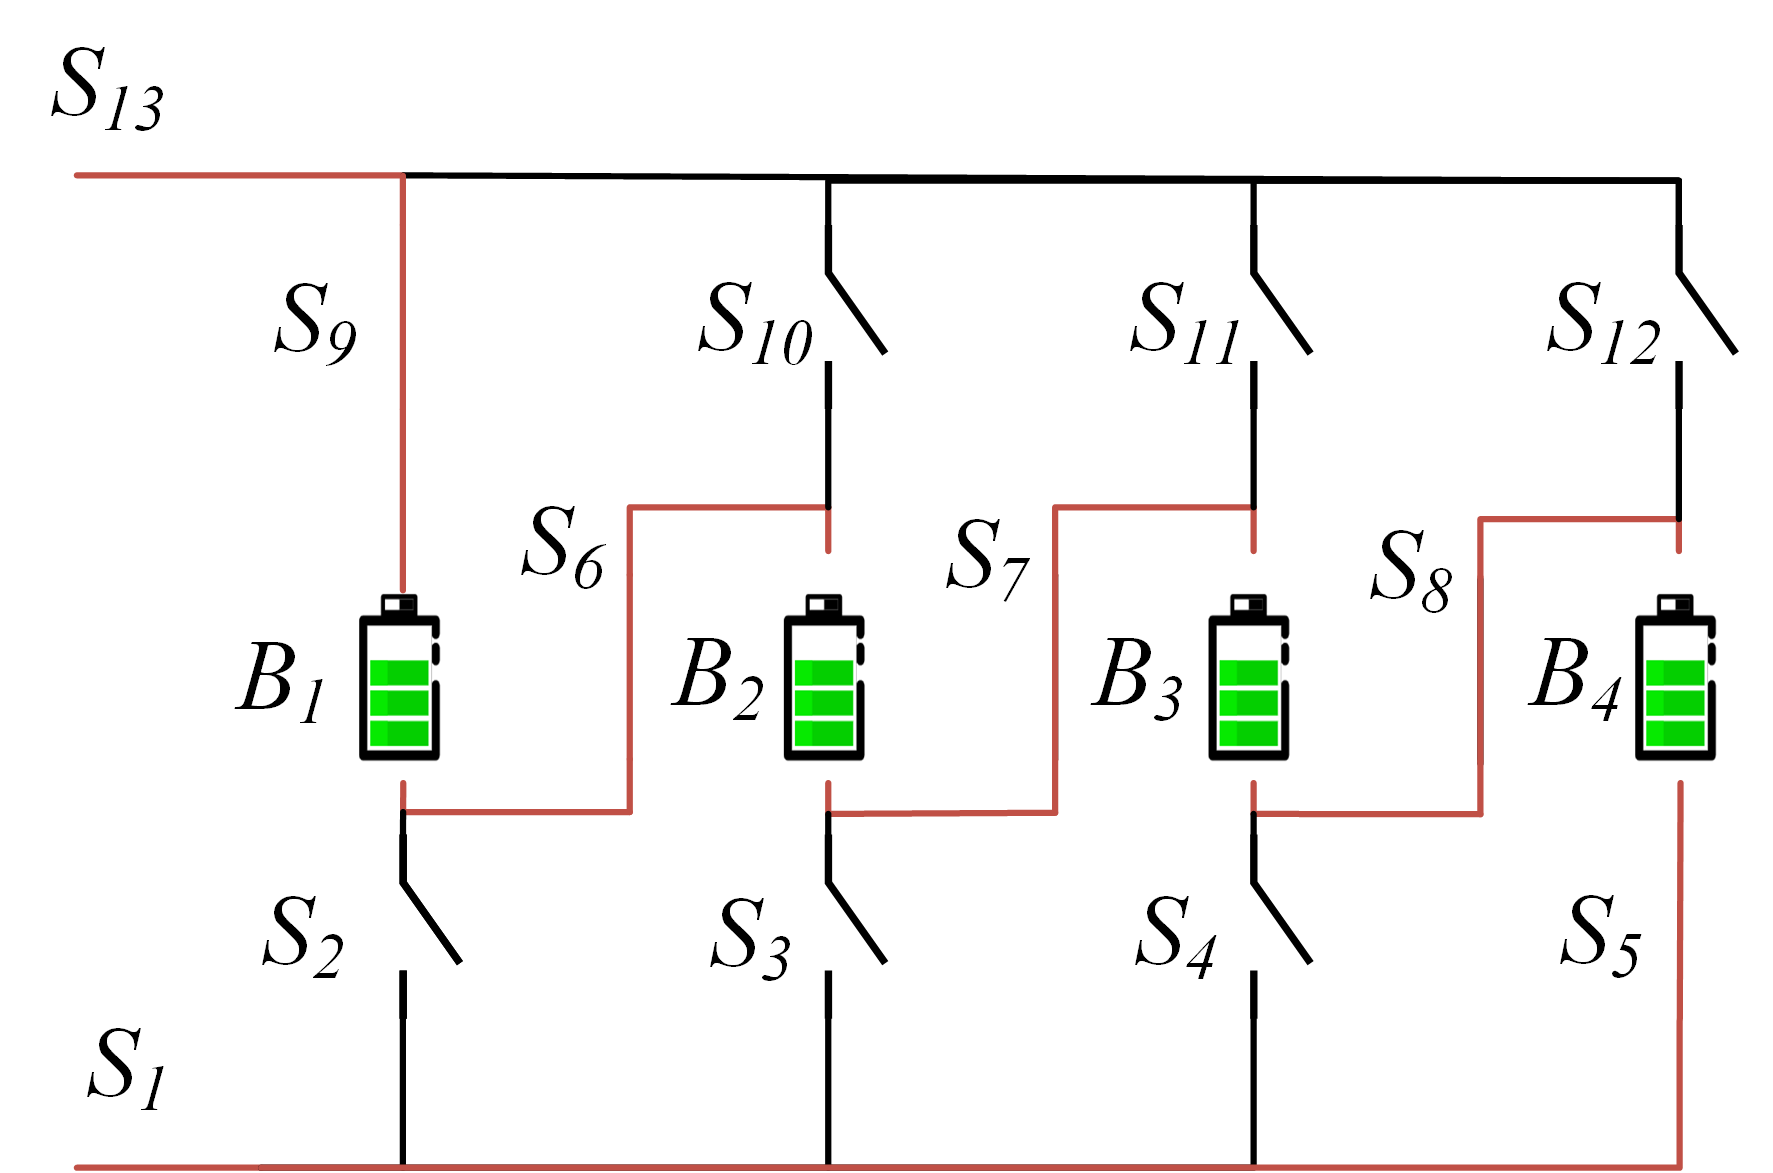
\includegraphics[width=\textwidth]{stru-V-serial.png}
        \caption{}
        \label{fig:stru-Visairo-serial}
    \end{subfigure}
    \\
    \begin{subfigure}[b]{0.45\textwidth}
        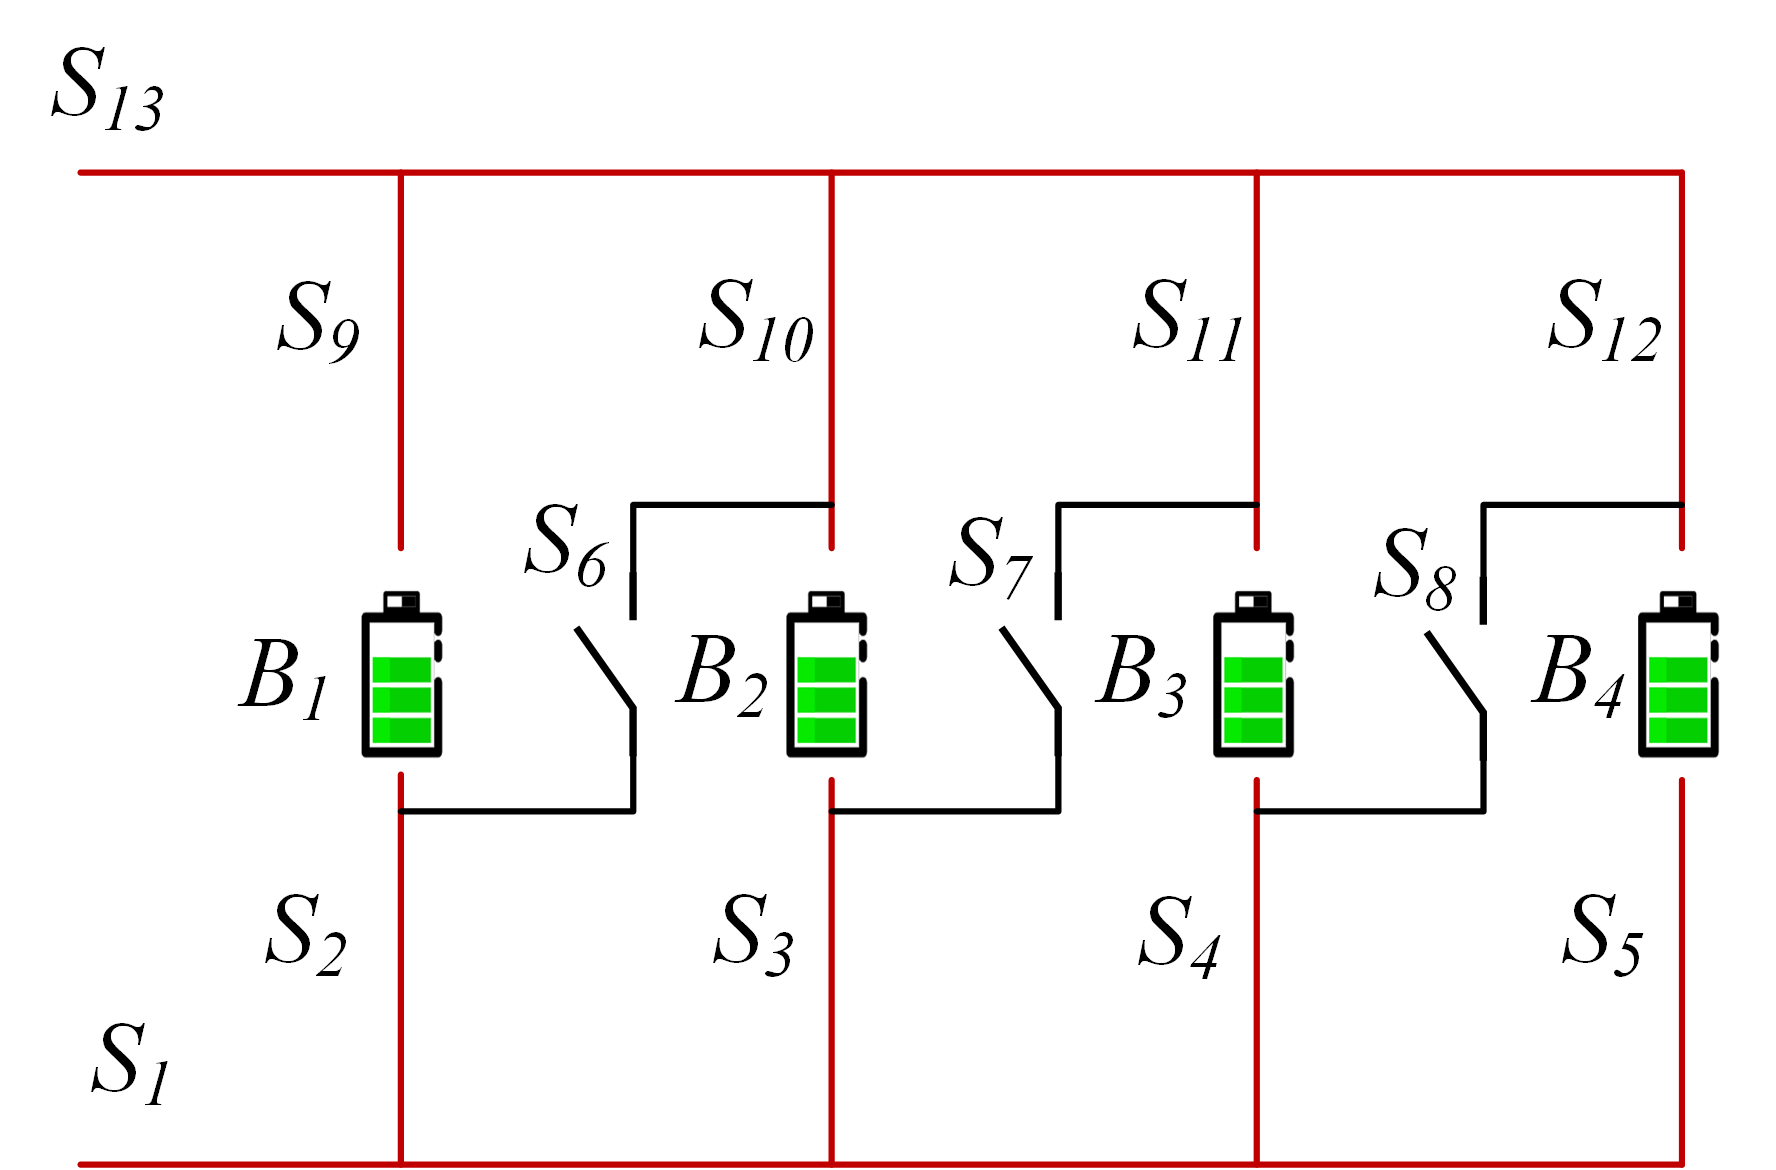
\includegraphics[width=\textwidth]{stru-V-parallel.png}
        \caption{}
        \label{fig:stru-Visairo-parallel}
    \end{subfigure}
    \hspace{0.05\textwidth}
    \begin{subfigure}[b]{0.45\textwidth}
        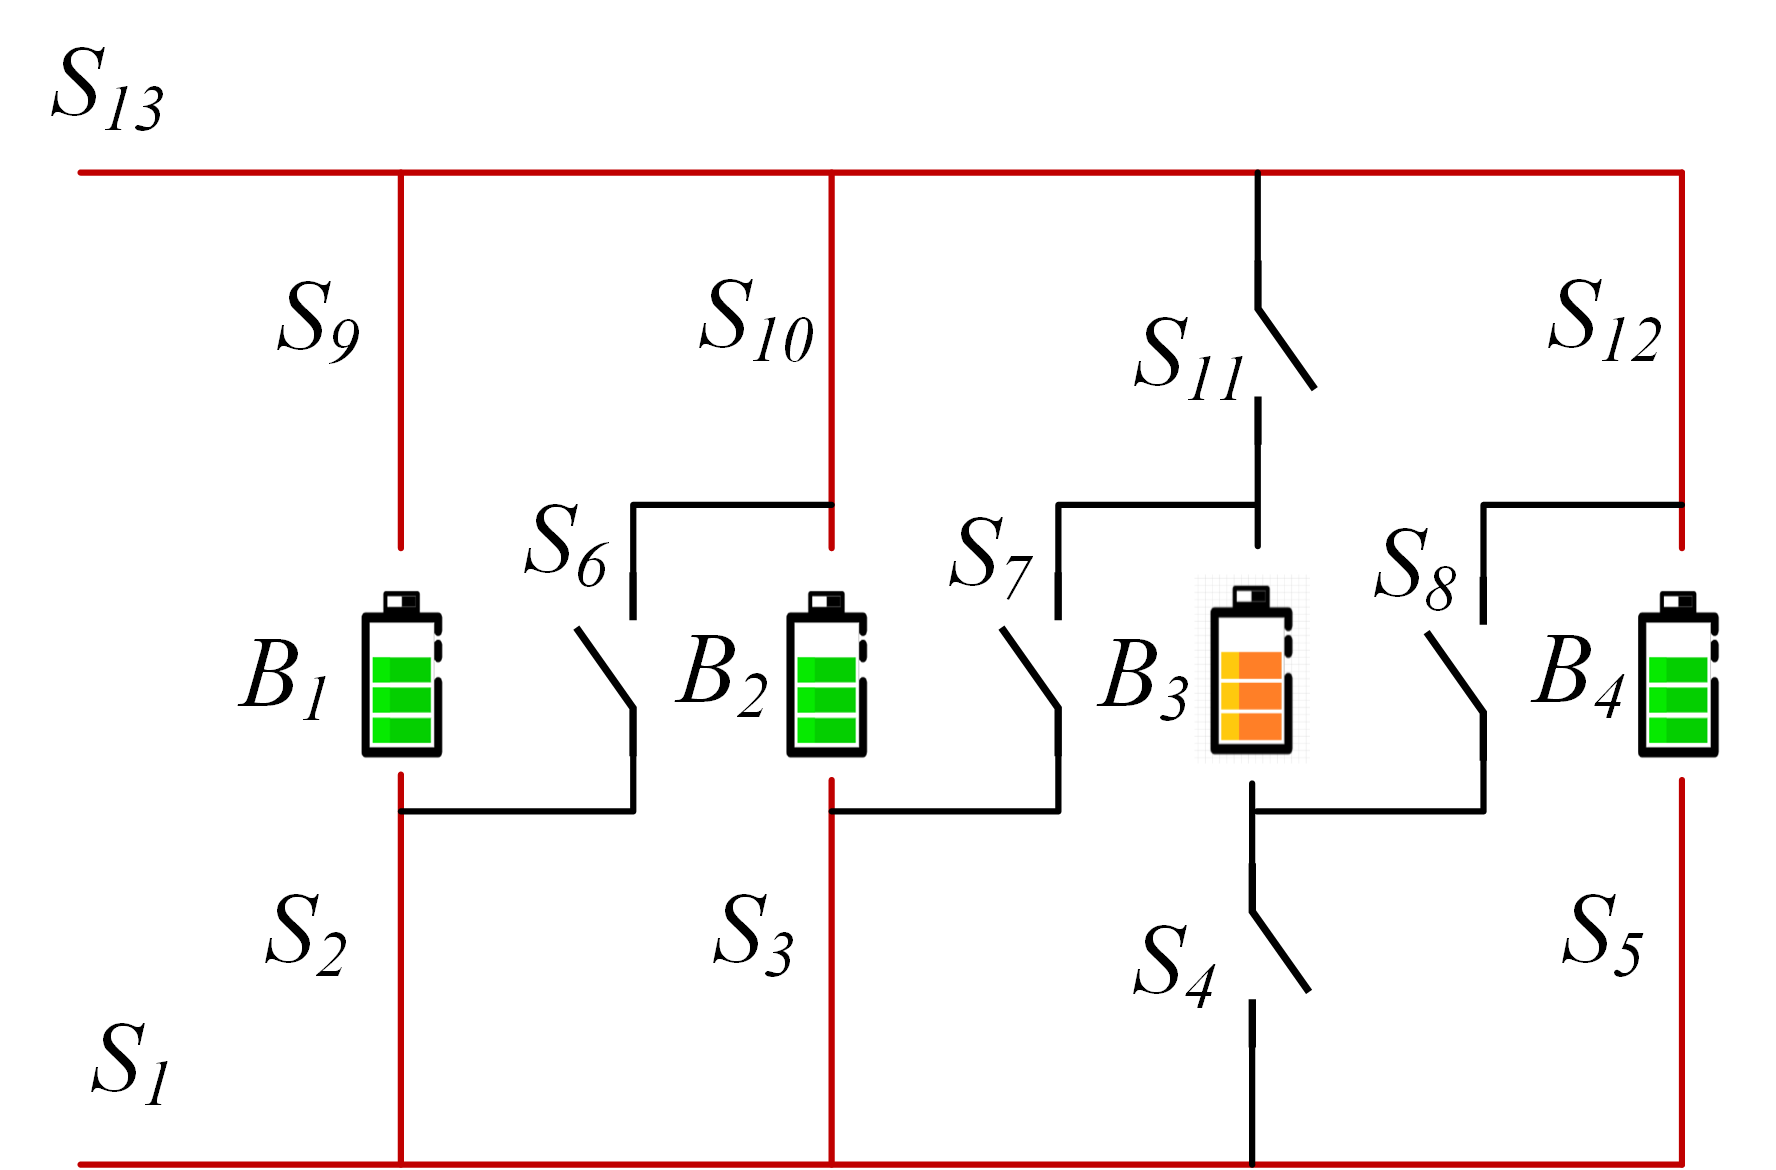
\includegraphics[width=\textwidth]{stru-V-isolate.png}
        \caption{}
        \label{fig:stru-Visairo-isolate}
    \end{subfigure}
    \caption{
        (a) The RBS structure proposed by Visairo\cite{visairoReconfigurableBatteryPack2008}, with
        all batteries in (b) series connection, (c) parallel connection, and
        (d) battery $B_3$ isolated.
        }
    \label{fig:arch}
\end{figure}

Recently, various types of RBSs with different flexibility and reconfigurability have been designed to meet application requirements. 
For example, Ci et al. \cite{ci2007novel} proposed an RBS structure that dynamically adjusts the battery discharge rate to fully exploit the available capacity of each battery. 
Jan's \cite{9209774,engelhardt2021double} structures  reconfigure structures with variant batteries in series to reach the (constantly changing) voltage requirements during electric vehicle charging.
As shown in Fig. \ref{fig:stru-Visairo}, the structure proposed by Visairo et al. \cite{visairoReconfigurableBatteryPack2008}  changes the system's output voltage based on the load conditions, thereby reducing the power loss of the voltage regulator during the power supply process and improving the efficiency of energy use. 
Also, to enhance the energy efficiency of the system, Lawson et al. \cite{lawsonSoftwareConfigurableBattery2012} and He et al. \cite{he2014reconfiguration}  proposed simplified structures that have fewer switches than Visairo's design.
Kim et al. \cite{kim2009dynamic} improved the system's ability to recover from battery failures by introducing multiple ports into the structure. 


The complex structure between batteries and switches gives RBSs flexibility but also creates challenges in the design and control of the system. 
Thus, several approaches to analyze the RBS structure and performance have been proposed to tackle these challenges.
For instance, 
Han et al. \cite{han2021analysis} derived an analytical expression for the maximum switch current during battery system reconfiguration for a specific RBS structure. 
This helps guide the selection of switches and supports the design of RBS hardware.
Chen et al. \cite{chenSneakCircuitTheory2021} proposed a systematic approach based on  sneak circuit theory to fundamentally avoid the short-circuit problem of RBSs: 
They thoroughly analyzed all paths between the cathode and anode of each battery in the RBS and identified paths that only contain switches as short-circuit paths for pre-checking before system reconfiguration. 


In spite of the maximum switch current mentioned above, the maximum allowable current (MAC), defined as the maximum allowed current  under the constraints of the battery cell, is another critical indicator of RBSs that needs to be evaluated during the design or control  of the system. 
The MAC helps the designers assess whether the RBS meets the output current requirements and contributes to the formulation of appropriate and safe management strategies for the battery management system.
Unfortunately, few studies have analyzed the RBS structure to determine the RBS MAC.
An intuitive and straightforward method is to enumerate all possible switch states and calculate the output current of the system under each reconfigurated structure.
However, this method is inefficient and time-consuming, especially for RBSs with a large number of switches.


To solve this issue, this paper proposes an efficient method to evaluate the MAC of RBSs. 
In this method, a greedy algorithm is designed to efficiently search the possible circuit topology of RBSs with MAC.
This algorithm transforms the enumeration of switch states in the brute-force algorithm into the combination of the batteries' shortest paths.
An improved direct graph model that considers the voltage, the internal resistance, the MAC of the battery, and the external load is also introduced to analyze the current of the RBS.
The main contributions of this paper can be summarized as follows:
\begin{itemize}
  \item An efficient method is proposed to determine the MAC of RBSs with arbitrary structures, including scenarios with isolated batteries.
  \item A greedy algorithm is applied to solve the MAC problem, the computational complexity of which is greatly reduced compared with the brute-force algorithm.
  \item An improved directed graph model is introduced to provide a specific method for calculating the MAC of a given structure.
\end{itemize}


The remainder of this paper is organized as follows: 
Section II presents the framework and details of the proposed directed graph model and  greedy algorithm. 
Section III discusses a case study that uses the proposed method to determine the MACs of two published four-battery RBSs and one with a more complex structure. 
The calculation results, the algorithm's computational complexity, and scenarios such as battery random isolation are also discussed. 
Finally, the concluding remarks are presented in Section IV.

\section{Methodology}

The central principle of this method is to connect the batteries in an RBS in parallel to the extent possible, thereby maximizing the output current of the RBS.
To achieve this universally and automatically, the overall process is divided into the four steps shown in Fig. \ref{fig:main}.
First, a directed graph model is established for subsequent computations. The model not only contains the connected relationships between batteries and switches but also retains the performance parameters of the batteries.
Subsequently, based on the equivalent circuit, the MAC problem is transformed into specific objective functions and constraints.
The shortest paths (SPs, where additional batteries and switches on the path are penalized as distance) for the batteries are then obtained  by using the Dijkstra algorithm to connect the batteries in the RBS in parallel.
Finally, a greedy algorithm is used to organize the switches, allowing the batteries to connect via their SPs while satisfying the constraints, resulting in the MAC of the RBS.

\begin{figure}[htbp]
    \centering
    \begin{subfigure}[b]{0.8\textwidth}
        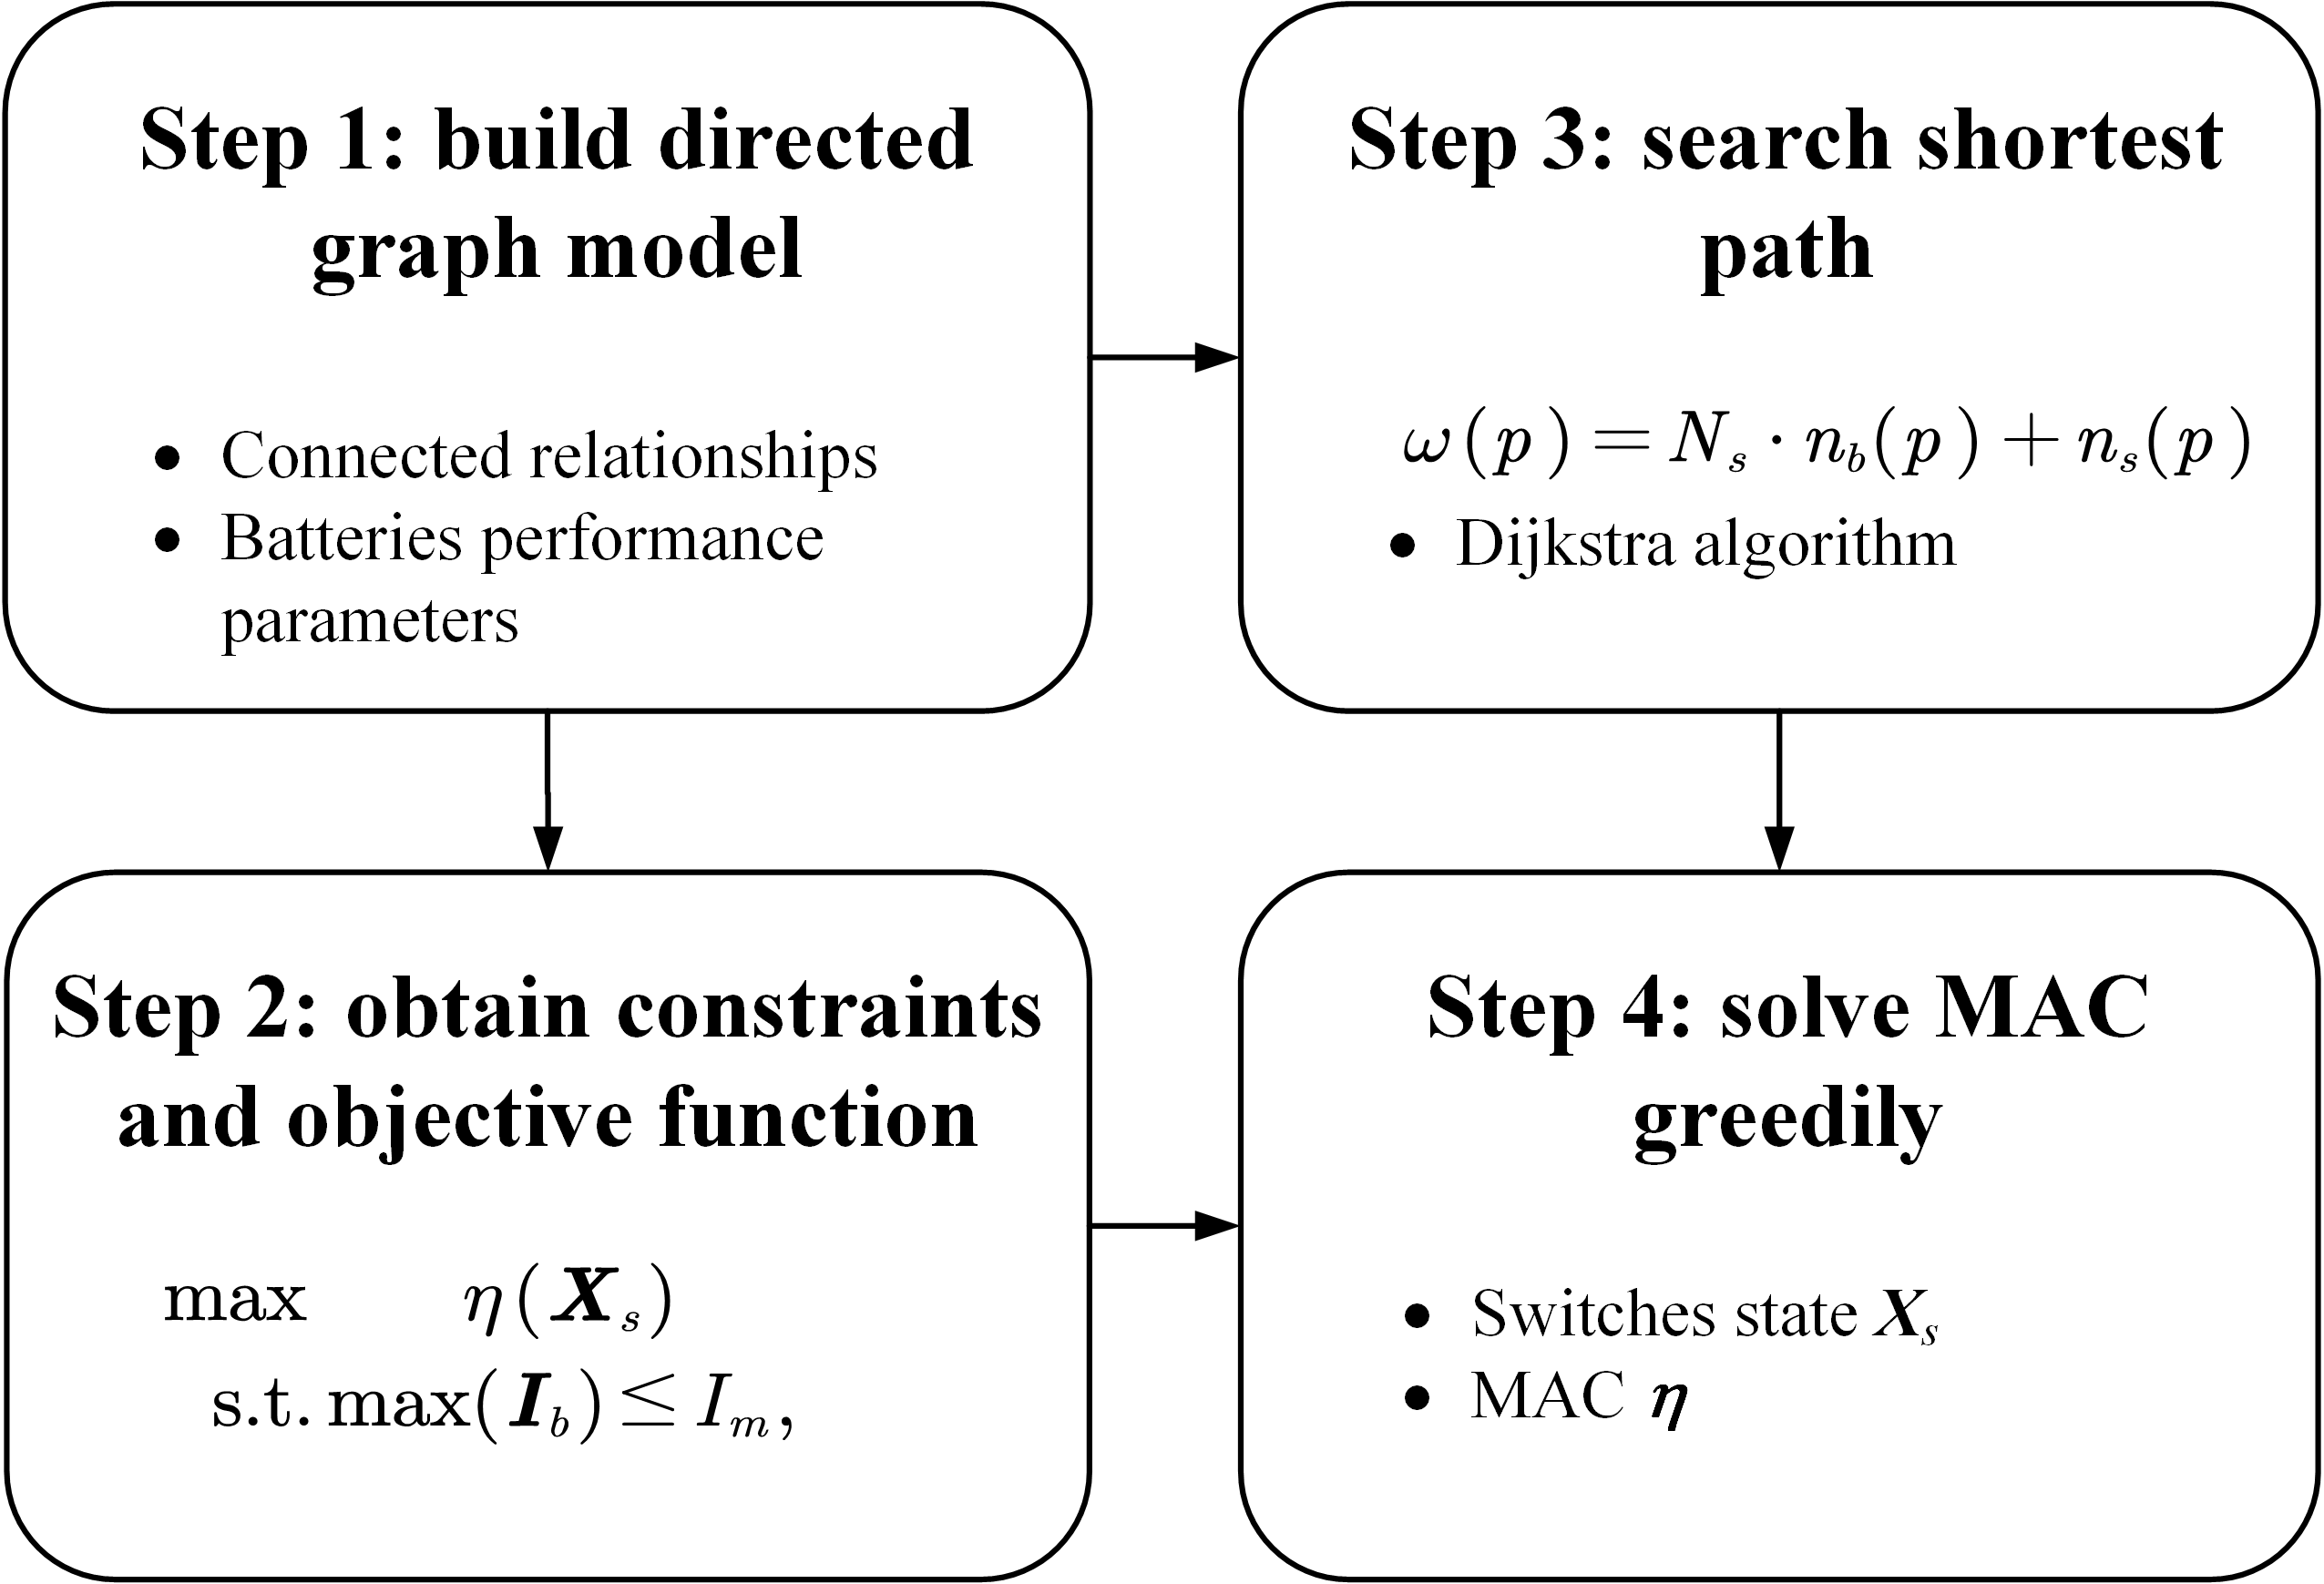
\includegraphics[width=\textwidth]{main.png}
    \end{subfigure}
    \caption{ 
        Diagram of this method, which contains four main steps.
    }
    \label{fig:main}
\end{figure}

\subsection{Directed graph model}

\begin{figure}[htbp]
    \centering
    \begin{subfigure}[b]{0.31\textwidth}
        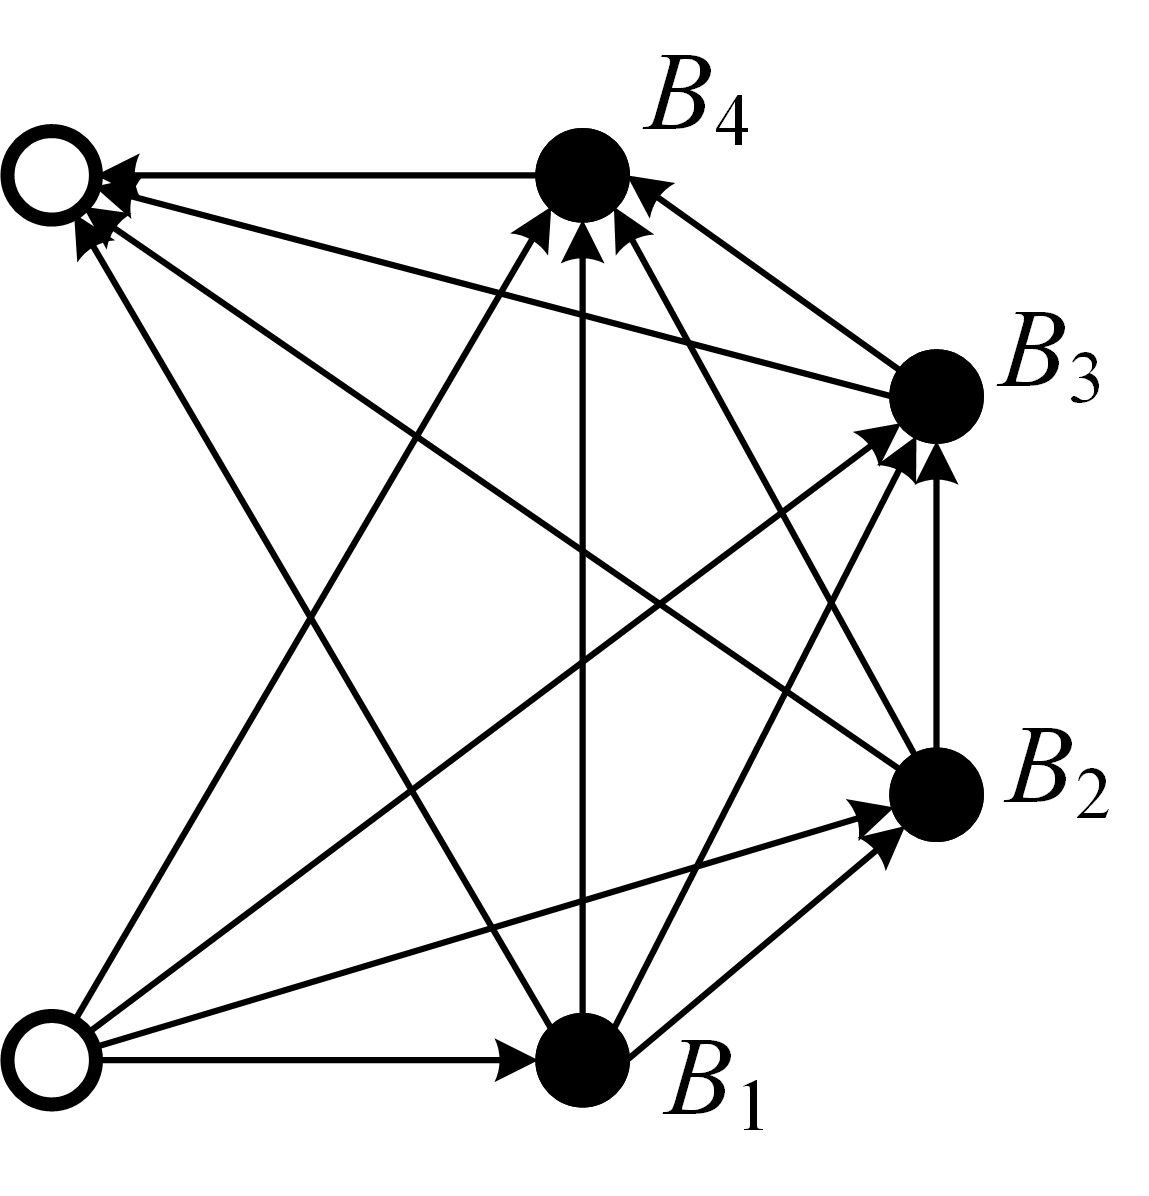
\includegraphics[width=\textwidth]{direct-graph-he.png}
        \caption{}
        \label{fig:direct-graph-he}
    \end{subfigure}
    \hspace{0.02\textwidth}
    \begin{subfigure}[b]{0.23\textwidth}
        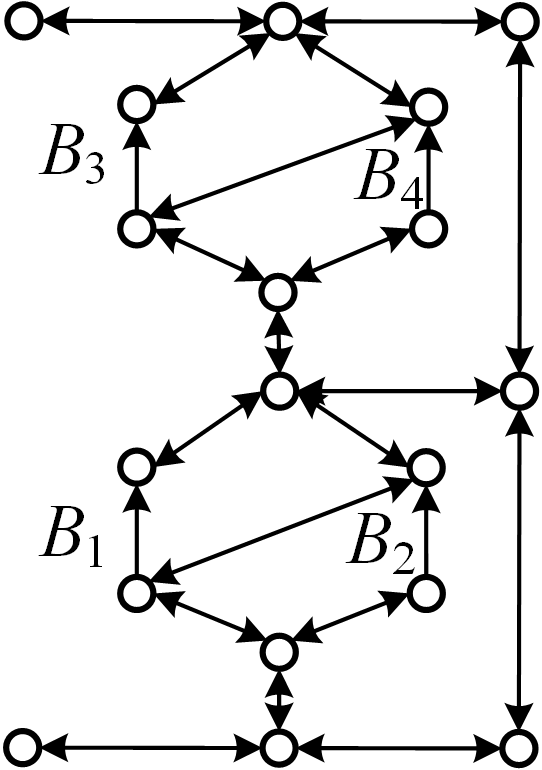
\includegraphics[width=\textwidth]{direct-graph-xu.png}
        \caption{}
        \label{fig:direct-graph-xu}
    \end{subfigure}
    \hspace{0.02\textwidth}
    \begin{subfigure}[b]{0.24\textwidth}
        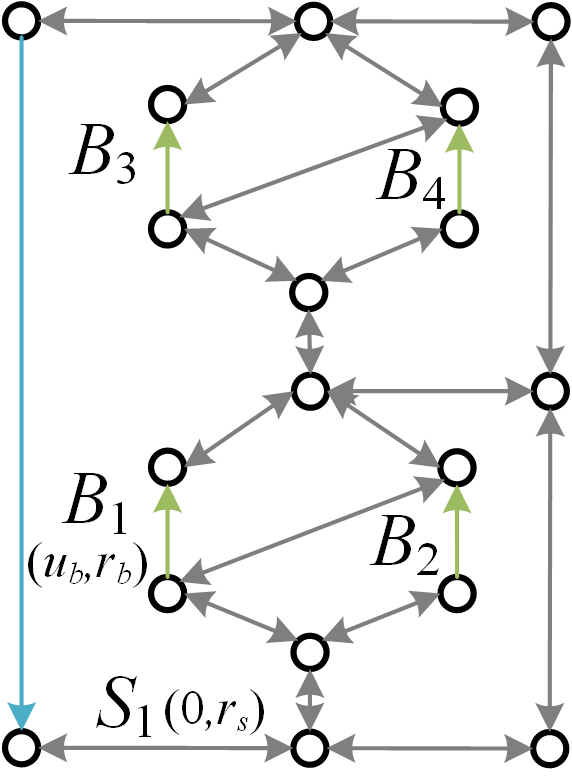
\includegraphics[width=\textwidth]{direct-graph-my.png}
        \caption{}
        \label{fig:direct-graph-my}
    \end{subfigure}
    \\
    \begin{subfigure}[b]{0.8\textwidth}
        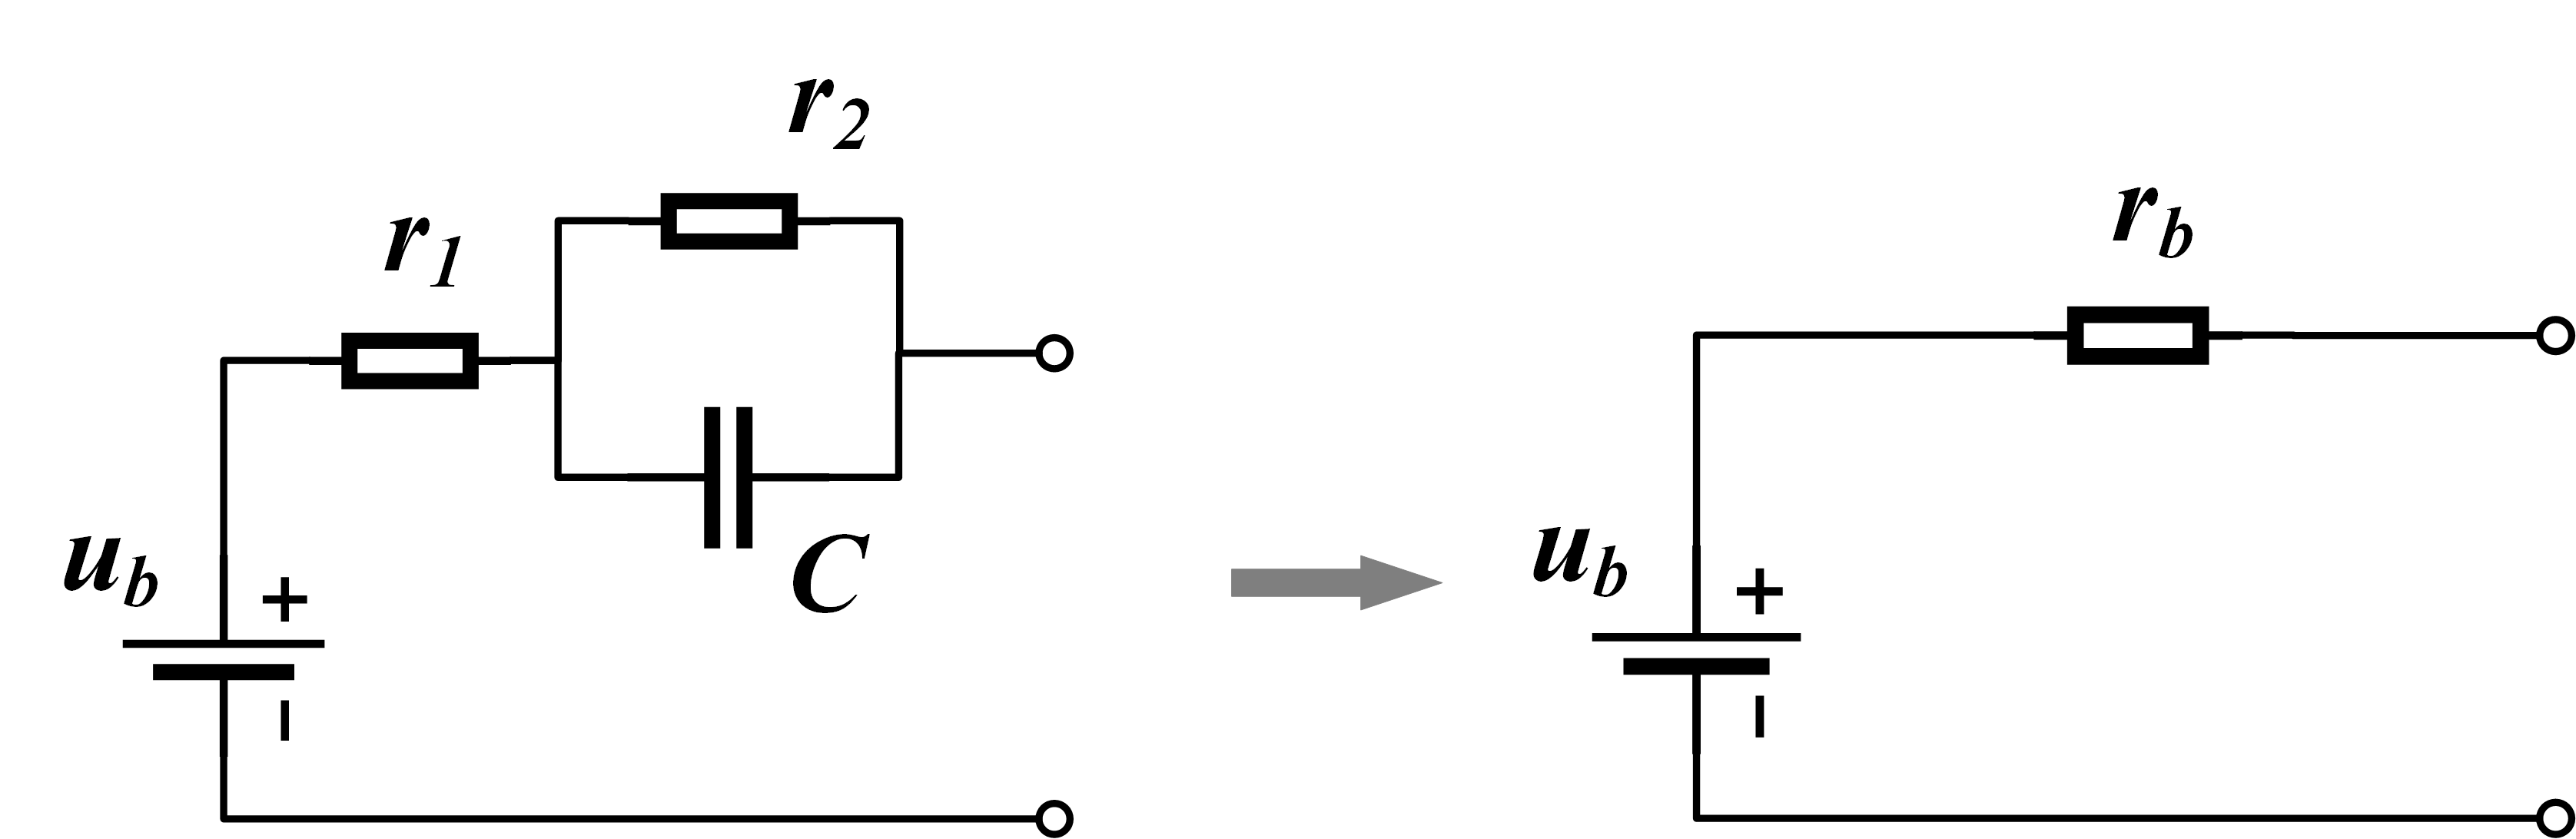
\includegraphics[width=\textwidth]{battery_simple.png}
        \caption{}
        \label{fig:battery_simple}
    \end{subfigure}
    \caption{ 
        Directed graph models used in (a) He's work \cite{heExploringAdaptiveReconfiguration2013}, (b) our previous work, and (c) the improved model in this paper.
        (d) The equivalent circuit of a battery in this method.
    }
\end{figure}

He et al. \cite{heExploringAdaptiveReconfiguration2013} proposed an abstracted directed graph model for an RBS, where the nodes represent the batteries, the edges represent the configuration flexibility, and the weight of each vertex corresponds to the battery voltage (Fig. \ref{fig:direct-graph-he}). 
The model captures all potential system configurations and offers a direct metric for configuration flexibility, but it does not specify the physical implementation of the connectivity between batteries, meaning that one graph might correspond to multiple RBS structures.
We previously proposed a directed graph model that differs completely from He's model by using nodes to represent the connections between batteries and switches and directed edges to represent batteries and switches (Fig. \ref{fig:direct-graph-xu}), allowing for a one-to-one correspondence between the RBS structure and the directed graph model. 
This model accurately and comprehensively represents the RBS topological structure but cannot be used for quantitative MAC calculations because it does not consider  the voltage, internal resistance, and MAC of the battery. 
To address this issue, we improve our previous model by adding electromotive force and resistance attributes on the edges based on its equivalent circuits.
The model also considers the external load as an equivalent resistance and integrates it into the analysis, making it a complete circuit model for later circuit analyses.
Fig. \ref{fig:direct-graph-my} shows the improved directed graph model used in this paper.
The following  provides a detailed explanation of the method for equating components in RBSs and constructing the directed graph model.


To use circuit analysis methods to solve the MAC of the RBS, the components in the RBS are equated to ideal circuit elements.
For instance, as shown in Fig. \ref{fig:battery_simple}, the battery in the RBS is represented as a black-box circuit consisting of two resistors $r_1$ and $r_2$ and a capacitor $C$, known as the Thevenin model \cite{hongwenheStateofChargeEstimationLithiumIon2011,mousavig.VariousBatteryModels2014}.
With an emphasis on the stable output of the RBS, the capacitor in the Thevenin model can be considered as an open circuit without affecting the steady-state current.
Therefore,  battery $B_i$ in the RBS can be simplified as a series connection between a constant voltage source $u_{i}$ and a resistor $r_{i}$.
Furthermore, the state of switch $S_j$ in the RBS is represented by a binary variable $x_j$, where 0 is ON and 1 is OFF.
When the switch is closed, the circuit can be regarded as a resistor with a very small resistance $r_{j}$.
Finally, the external load is considered as a resistor with resistance $R_o$.


For a given RBS structure, its directed graph model $G(V,E)$ is constructed as follows:
\begin{enumerate}
    \item Nodes:
        The nodes in the directed graph correspond to the connection points of components in the actual RBS. 
        Assuming there are a total of $N$ nodes in the RBS, for the sake of convenience, the anode of the RBS is denoted as $v_1$ and the cathode as $v_N$.
    \item Edges:
        The edges in the directed graph correspond to the batteries, switches, and external electrical loads in the actual RBS.
        Therefore, there are three types of directed edges. 
        For battery $B_i$, its directed edge $e_i$ is drawn from the cathode to the anode because the battery in operation only allows current to flow in one direction.
        For switch $S_j$, since it is allowed to work under bidirectional currents, it is represented by a pair of directed edges with two-way directions. 
        Regarding the external electronic load, because it is connected to the anode and cathode of the RBS, a directed edge from $v_N$ to $v_1$  represents it. 
        In conclusion, for a given RBS structure with $N_b$ batteries and $N_s$ switches, the number of directed edges is $N_b+2N_s+1$, where 1 refers to the external electrical load.
    \item Attributes of edges:
        Each edge is assigned two attributes, voltage difference and resistance, based on the equivalent method mentioned above.
        The values for  battery $B_i$, switch $S_j$, and external loads correspond to $(u_i, r_i)$, $(0, r_j)$, and $(0, R_o)$, respectively.
\end{enumerate}

\subsection{Constraints and objective function}

For a given RBS, determining its MAC involves maximizing the RBS output current while ensuring that all battery currents do not exceed the batteries' MAC. 
This subsection establishes the constraints and objective function to determine the RBS's MAC through circuit analysis based on the directed graph model provided in the previous section.


First, the topology in the directed graph model is represented in matrix form $\bm{A}$, known as the incidence matrix and defined as follows:
\begin{align}\label{eq:A}
    a_{kl}=
    \begin{cases}
        1,  & \text{edge $l$ leaves node $k$},\\
        -1, & \text{edge $l$ enters node $k$},\\
        0,  & \text{otherwise}.
    \end{cases}
\end{align}
For a directed graph consisting of $N$ nodes and $N_b+2N_s+1$ directed edges, its incidence matrix $\bm{A}$ is an $N\times(N_b+2N_s+1)$ matrix. 
In this matrix, the rows and columns represent the nodes and edges of the directed graph, respectively.
By distinguishing the components in the RBS corresponding to each column, $\bm{A}$ can be rewritten as
\begin{equation}\label{eq:A_bso}
    \bm{A} =
    \begin{bmatrix}
        \bm{A}_b & \bm{A}_s & \bm{A}_o
    \end{bmatrix},
\end{equation}
where $\bm{A}_b$, $\bm{A}_s$, and $\bm{A}_o$ are the submatrices corresponding to the batteries, switches, and external electrical load, respectively.
To reduce the computational complexity, the dimensions of matrix $\bm{A}$ are reduced.
Since each directed edge has one node to leave and one to enter, the values in every column of $\bm{A}$ sum to zero.
Therefore, removing the last row will not result in a loss of information. 
Conversely, since each switch in the RBS is represented by a pair of directed edges with two-way directions, the two columns corresponding to the switch are mutually opposite.
Thus, for the submatrix $\bm{A}_s$, only one column is retained for each pair of columns representing the same switch.
As a result, $\bm{A}$ can be reduced to an $(N-1)\times(N_b+N_s+1)$ matrix, denoted  $\bm{\tilde{A}}$, for further calculation of current and voltage.
Similar to Eq. (\ref{eq:A_bso}), $\bm{\tilde{A}}$ can be rewritten as
\begin{equation}\label{eq:A_bso_tilde}
    \bm{\tilde{A}} =
    \begin{bmatrix}
        \bm{\tilde{A}}_b & \bm{\tilde{A}}_s & \bm{\tilde{A}}_o
    \end{bmatrix}.
\end{equation}


After obtaining the incidence matrix, the currents of all batteries and output in the RBS are determined by solving the circuit equations.
According to Kirchhoff's laws, we have
\begin{align}\label{eq:Kirchhoffs_law}
    \begin{cases}
        \bm{\tilde{A}} \bm{I} = \bm{0}, \\
        \bm{U}        = \bm{\tilde{A}}^\T \bm{U}_n,
    \end{cases}
\end{align}
where $\bm{I}$ and $\bm{U}$ indicate the current and voltage difference arrays of the $N_b+N_s+1$ edges, respectively, and
$\bm{U}_n$ is the voltage array of the $N-1$ nodes.
These directed edges are treated as generalized branches and expressed in matrix form as follows:
\begin{equation}\label{eq:generalized_branches}
    \bm{I} = \bm{Y}\bm{X} \bm{U} - \bm{Y}\bm{X} \bm{U}_s +\bm{I}_s,
\end{equation}
where $\bm{U}_s$ and $\bm{I}_s$ denote the source voltage and source current of the generalized branches, respectively.
Because all batteries have been equivalent to voltage sources rather than current sources in the previous subsection, all elements of the array $\bm{I}_s$ are zero, 
whereas the elements of the array $\bm{U}_s$ are equal to the first attribute of the corresponding edges in the directed graph.
The matrix $\bm{Y}$ in Eq. (\ref{eq:generalized_branches}) is the admittance matrix of the circuit and is defined as the inverse of the impedance matrix.
The elements on the diagonal of matrix $\bm{Y}$ are equal to the reciprocal of the resistance, which is the second attribute of the corresponding edges in the directed graph. The off-diagonal elements of $\bm{Y}$ are zero.
$\bm{X}$ is the state matrix that determines whether the RBS batteries and switches can pass current.
It is defined as
\begin{equation}\label{eq:X}
    \bm{X} = \diag(
    \underbrace{1, 0, \dots, 1}_{N_b~\text{of}~0/1},
    \underbrace{1, 0, \dots, 1}_{N_s~\text{of}~0/1},
    1)
    =\begin{bmatrix}
        \bm{X}_b & & \\
        & \bm{X}_s &\\
        & & 1
    \end{bmatrix},
\end{equation}
where element $x_i$ of matrix $\bm{X}_b$ indicates whether battery $B_i$ has been removed from the circuit, with $x_i=1$ indicating removal and $x_i=0$ indicating that battery $B_i$ is still available to supply power. 
When all batteries are healthy and capable of providing current to the external load, $\bm{X}_b$ is the identity matrix. 
The elements $x_j$ of  matrix $\bm{X}_s$ determine whether switch $S_j$ is closed, with $x_j=1$ indicating a closed switch and $x_j=0$ indicating an open switch, which is consistent with the previous subsection.


Theoretically, the output current $I_o$ and the currents of each battery $\bm{I}_b$ in the RBS  can be determined by solving Eqs. (\ref{eq:Kirchhoffs_law})--(\ref{eq:X}) under any given state $\bm{X}$.
To further simplify the problem, it is assumed that all batteries have the same electromotive force and internal resistance, which are denoted $u_b$ and $r_b$, respectively.
This allows us to derive explicit expressions for $I_o$ and $\bm{I}_b$.
After derivation and simplification, the output current $I_o$ and the currents of each battery $\bm{I}_b$ are ultimately represented as Eqs. (\ref{eq:I_o}) and (\ref{eq:I_b}), respectively:
\begin{equation}\label{eq:I_o}
    I_o = \frac{1}{R_o r_b} \bm{\tilde{A}}_o^\T \bm{Y}_n^{-1}(\bm{X}) \bm{\tilde{A}}_b \bm{U}_b,
\end{equation}
\begin{equation}\label{eq:I_b}
    \bm{I}_b = \frac{1}{r_b^2}[\bm{\tilde{A}}_b^\T \bm{Y}_n^{-1}(\bm{X}) \bm{\tilde{A}}_b\bm{U}_b -r_b \bm{U}_b],
\end{equation}
where $\bm{U}_b$ is an $N_b\times 1$ array with all elements equal to $u_b$,
and $\bm{Y}_n$ is the equivalent admittance matrix of the circuit and is defined as
\begin{equation}\label{eq:Yn}
    \bm{Y}_n (\bm{X}) = \frac{1}{R_o} \bm{\tilde{A}}_o\bm{\tilde{A}}_o^\T + \frac{1}{r_b} \bm{\tilde{A}}_b\bm{X}_b\bm{\tilde{A}}_b^\T + \frac{1}{r_s}\bm{\tilde{A}}_s\bm{X}_s\bm{\tilde{A}}_s^\T.
\end{equation}


To characterize the current output capacity of the RBS structure under different switching states, an indicator $\eta$ is defined by the ratio of $I_o$ to $\max (\bm{I}_b)$:
\begin{equation}\label{eq:eta}
    \eta = \frac{I_o}{\max (\bm{I}_b)}.
\end{equation}
Finally the problem of finding the MAC can be formulated as
\begin{align}
    & \max \eta(\bm{X}_s) \label{eq:max_eta}\\
    \text{s.t. } & \max (\bm{I}_b) \leq I_m, \label{eq:Ib_leq_Im}
\end{align}
where $I_m$ is the MAC of the battery.


However, it remains computationally difficult to solve Eq. (\ref{eq:max_eta}) because of $\bm{Y}_n^{-1}$.
On one hand,  the introduction of nonlinear terms by $\bm{Y}_n^{-1}$ renders many  methods in linear optimization unsuitable for this problem.
On the other hand, the rank of $Y_{n}$ is proportional to the number of batteries and switches, which can be very large for a large RBS, leading to a significant computational burden.
As a result, intelligent algorithms that rely on evolution by iteration may face efficiency problems when dealing with a large RBS.
To address this issue, the problem should be considered from the perspective of guiding the RBS to reconstruct as many parallel structures as possible.
Consequently, a greedy algorithm based on the shortest path is proposed. 
The detailed implementation of this algorithm is presented in the following two subsections.

\subsection{Shortest path}

The path $p$ used in this method is defined as the complete route that passes through one battery (or a consecutive series of batteries) and closed switches, connecting the anode $v_1$ to the cathode $v_N$ of the RBS.
By applying a penalty to the series-connected batteries on the path, where additional batteries imply a greater distance, the algorithm encourages the RBS to form parallel structures to the extent possible.
In addition, to reduce the number of switches controlled during the reconstruction process, a penalty is also applied to the total number of switches on the path while ensuring the minimum number of batteries.
Therefore, the distance $\omega$ of path $p$ is  
\begin{equation}\label{eq:weight}
    \omega(p) = N_s  n_b (p) + n_s (p),
\end{equation}
where $N_s$ is the total number of switches in the system, 
and $n_b(p)$ and $n_s(p)$ are number of batteries and switches in path $p$, respectively. 
Moreover, the shortest path $SP_i$ is defined as the path with the minimum $\omega$ for battery $B_i$:
\begin{equation}\label{eq:def_sp}
    SP_i = \mathop{\arg\min}_{p \in P_i} \omega(p),
\end{equation}
where $P_i$ is the set of all paths from $v_1$ to $v_N$ that pass through directed edge $i$.


$SP_i$ can be solved by the Dijkstra algorithm.
The Dijkstra algorithm is a graph-search method that finds the shortest path between two given nodes in a weighted graph, efficiently solving the single-source shortest-path problem.
Denoting the cathode and anode of battery $B_i$ as $v_i^-$ and $v_i^+$ respectively, then path $p$ of battery $B_i$  can be divided into three segments: $v_1 \rightarrow v_i^-$, $v_i^+ \rightarrow v_N$, and $v_i^- \rightarrow v_i^+$. $v_i^- \rightarrow v_i^+$ is the directed edge corresponding to battery $B_i$. 
With the Dijkstra algorithm, shortest paths for $v_1 \rightarrow v_i^-$ and $v_i^+ \rightarrow v_N$ can be calculated under the weights given in Eq. (\ref{eq:weight}) and denoted $SP(v_i^- \rightarrow v_i^+)$ and $SP(v_i^+ \rightarrow v_N)$, respectively.
Finally, $SP_i$ for battery $B_i$ is formed by the complete path, which consists of $SP(v_1 \rightarrow v_i^-)$, $v_i^- \rightarrow v_i^+$, and $SP(v_i^+ \rightarrow v_N)$.

\subsection{Greedy algorithm}\label{subsec:greedy_solution}

From the perspective of series vs parallel connections, integrating more batteries into the circuit through their shortest paths (SPs) results in more batteries connected in parallel, thereby increasing the total output current of the RBS.
However, conflicts may arise between the SPs of different batteries. 
For instance, the SPs of two batteries might form a short-circuit RBS structure, which is not allowed. 
To address this issue, a greedy algorithm incorporates as many SPs as possible while satisfying the reconstruction requirements.

The algorithm (see pseudo-code in Algorithm 1) is illustrated in Fig. \ref{fig:flowchart} and is summarized as follows:
First, the SPs are obtained by using Eqs. (\ref{eq:weight}) and (\ref{eq:def_sp}) in conjunction with the Dijkstra search. 
Next, the matrix $\bm{A}$ is calculated using Eq. (\ref{eq:A}), and the initial $N_{\text{set}}$ is set to $N_b$. 
The algorithm uses a dichotomy method to iteratively check until convergence different combinations of $c_b$ batteries from $N_b$ and updates $N_{\text{set}}$. 
For each combination, the algorithm constructs an effective solution if possible and calculates the currents $I_o$ and $\bm{I}_b$ by using Eqs. (\ref{eq:I_o}) and (\ref{eq:I_b}). 
If the maximum current $\bm{I}_b$ is less than or equal to $I_m$, $\eta$ is calculated by using Eq. (\ref{eq:eta}), and the maximum $\eta$ is updated accordingly. 
Finally, the algorithm outputs the maximum $\eta$ once $N_{\text{set}}$ converges.

\tikzset{
  meta box/.style={draw, black, very thick, text centered, },
  punkt/.style={meta box, rectangle, rounded corners, inner sep=.25em, minimum height=2em, minimum width=4em, align=center, text width=10em },
  round/.style={meta box, circle, minimum size=0, inner sep=0pt, outer sep=0pt },
  every fit/.style={draw, thick, dashed, gray, inner xsep=.5em, inner ysep=.75em }
}
\begin{figure}
\begin{tikzpicture}[font=\small, node font=\small, node distance=1.5em]
    \node[punkt]     (input) {Input: RBS structure};
    \node[punkt, below=0.3of input] (get_SP) {get SPs by Eqs. (\ref{eq:weight}) and (\ref{eq:def_sp}) and Dijkstra Search};
    \node[punkt, below=0.3of get_SP] (get_A) {get $\bm{A}$ from Eq. (\ref{eq:A})};
    \node[punkt, below=0.3of get_A] (get_Nset) {init $N_{\text{set}}=N_b$ };
    \node[punkt, below=0.3of get_Nset] (get_cb) {get $c_b$s by combinating $N_{\text{set}}$ batteries from $N_b$};
    \node[draw, diamond, aspect=2, below=0.3of get_cb] (is_check_all_cb) {are all $c_b$s checked?};
    \node[draw, diamond, aspect=2, right=1of is_check_all_cb] (is_Nset_converged) {is $N_{\text{set}}$ converged?};
    \node[punkt, above=0.3of is_Nset_converged] (reset_Nset) {reset $N_{\text{set}}$ by dichotomy};
    \node[punkt, text width=15em, below=0.3of is_check_all_cb] (get_Xs) {
        select an unchecked $c_b$, and get its $\bm{X}_m$ by \\ 
        if switch $j$ $\in \bigcup_{i\in c_b}SP_i$:\\
        $\bm{X}[j]=1$ else $0$};
    \node[punkt, below=0.3of get_Xs] (get_Yn) {get $\bm{Y}_n$ by Eq. (\ref{eq:Yn})};
    \node[draw, diamond, aspect=2, below=0.3of get_Yn] (is_Yn_invertible) {is $\bm{Y}_n$ invertible?};
    \node[punkt, right=1.3of is_Yn_invertible] (construct) {construct an effective solution};
    \node[punkt, below=0.3of is_Yn_invertible] (get_I) {get $I_o$ and $\bm{I}_b$ by Eqs. (\ref{eq:I_o}) and (\ref{eq:I_b})};
    \node[draw, diamond, aspect=2, below=0.3of get_I] (is_leq_Im) {is $\max \bm{I}_b \leq I_m$?};
    \node[punkt, right=1.3of is_leq_Im] (drop_eta) {drop this $\eta$};
    \node[punkt, below=0.3of is_leq_Im] (get_eta) {get $\eta$ by Eq. (\ref{eq:eta})};
    \node[punkt, below=0.3of get_eta] (update_max_eta) {update $\max \eta$};
    \node[punkt, right=1of is_Nset_converged] (output) {Output: $\max \eta$};
    \node[round,left=1.5of update_max_eta](point1){};

    \graph{
      (input) -> (get_SP) -> (get_A) -> (get_Nset) -> (get_cb) -> (is_check_all_cb) ->["No"] (get_Xs) -> (get_Yn) -> (is_Yn_invertible) ->["Yes"] (get_I) -> (is_leq_Im) ->["Yes"] (get_eta) -> (update_max_eta);
      (is_check_all_cb) ->["Yes"] (is_Nset_converged) ->["No"] (reset_Nset) -> (get_cb);
      (is_Yn_invertible) ->["No"] (construct) ->[to path={|- (\tikztotarget)}] (get_I);
      (is_leq_Im) ->["No"] (drop_eta) ->[to path={|- (\tikztotarget)}] (update_max_eta);
      (is_Nset_converged) ->["Yes"] (output);
      (update_max_eta) -- (point1) ->[to path={|- (\tikztotarget)}] (is_check_all_cb);
    };
\end{tikzpicture}
\caption{The computational flowchart of the MAC for a given RBS.}\label{fig:flowchart}
\end{figure}

% \begin{figure}[htbp]
%     \centering
%     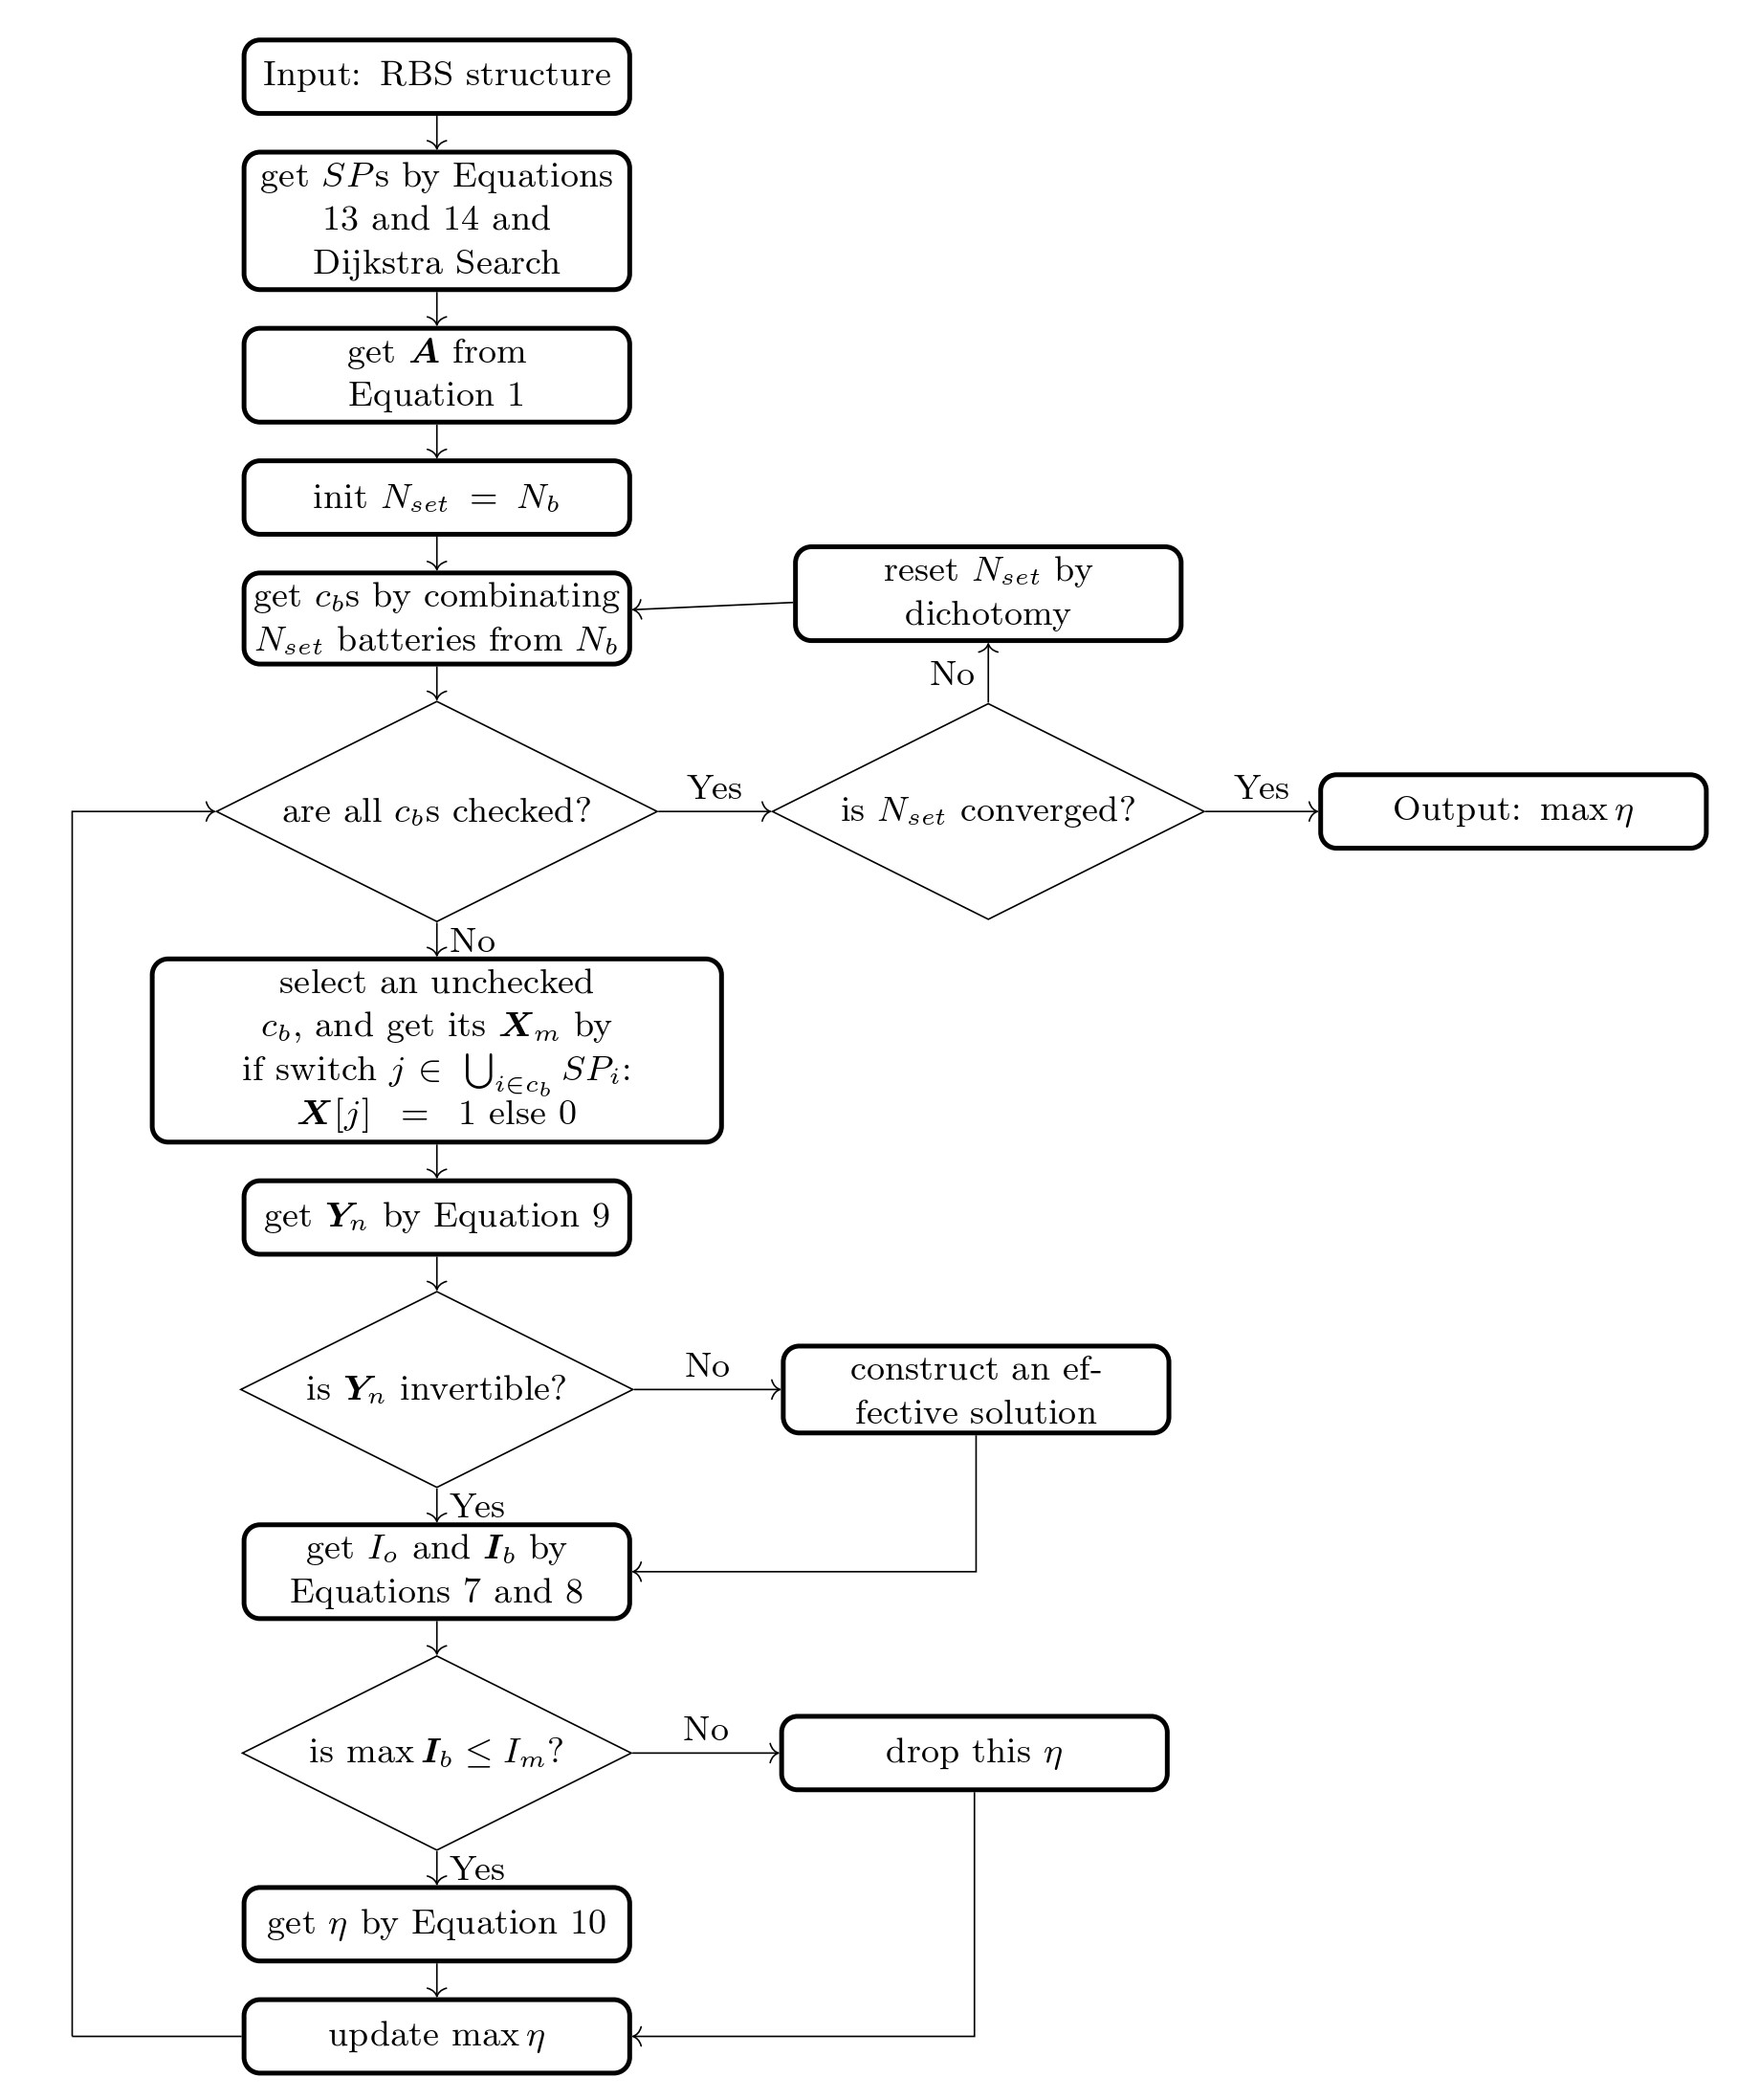
\includegraphics[width=\textwidth]{flowchart.jpg}
%     \caption{Computational flowchart of MAC for a given RBS.}\label{fig:flowchart}
% \end{figure}

\section{Case Study}

\subsection{Structures}

\begin{figure}[htbp]
    \centering
    \begin{subfigure}[b]{0.2\textwidth}
        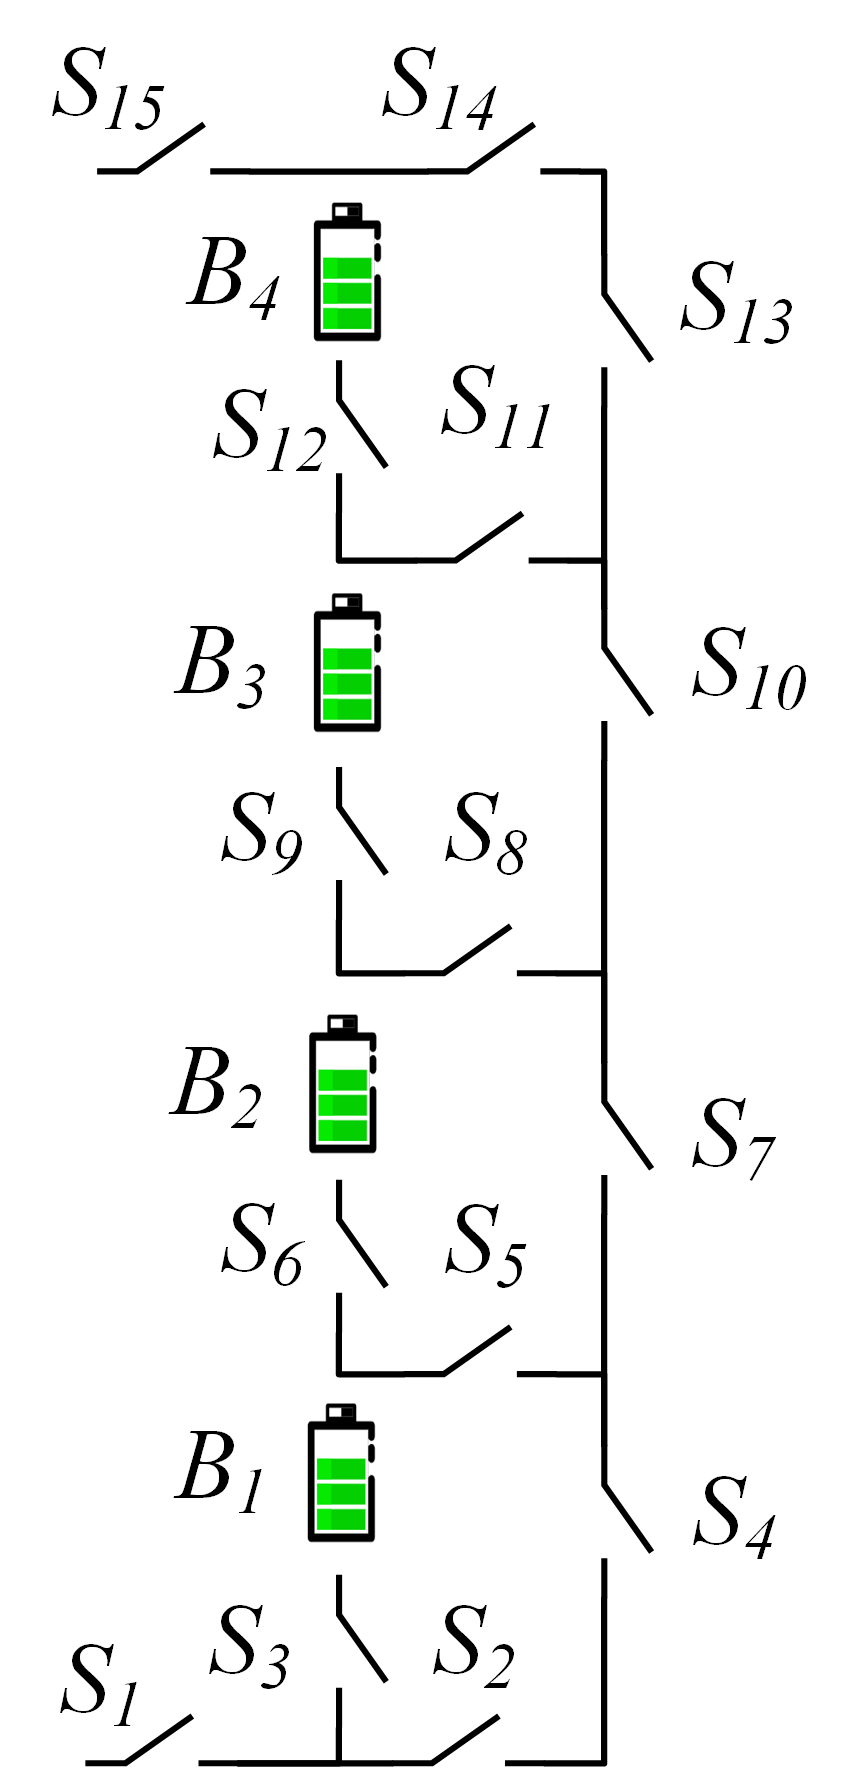
\includegraphics[width=\textwidth]{stru-L-origin.png}
        \caption{}
        \label{fig:study-stru-Lawson}
    \end{subfigure}
    \hspace{0.02\textwidth}
    \begin{subfigure}[b]{0.4\textwidth}
        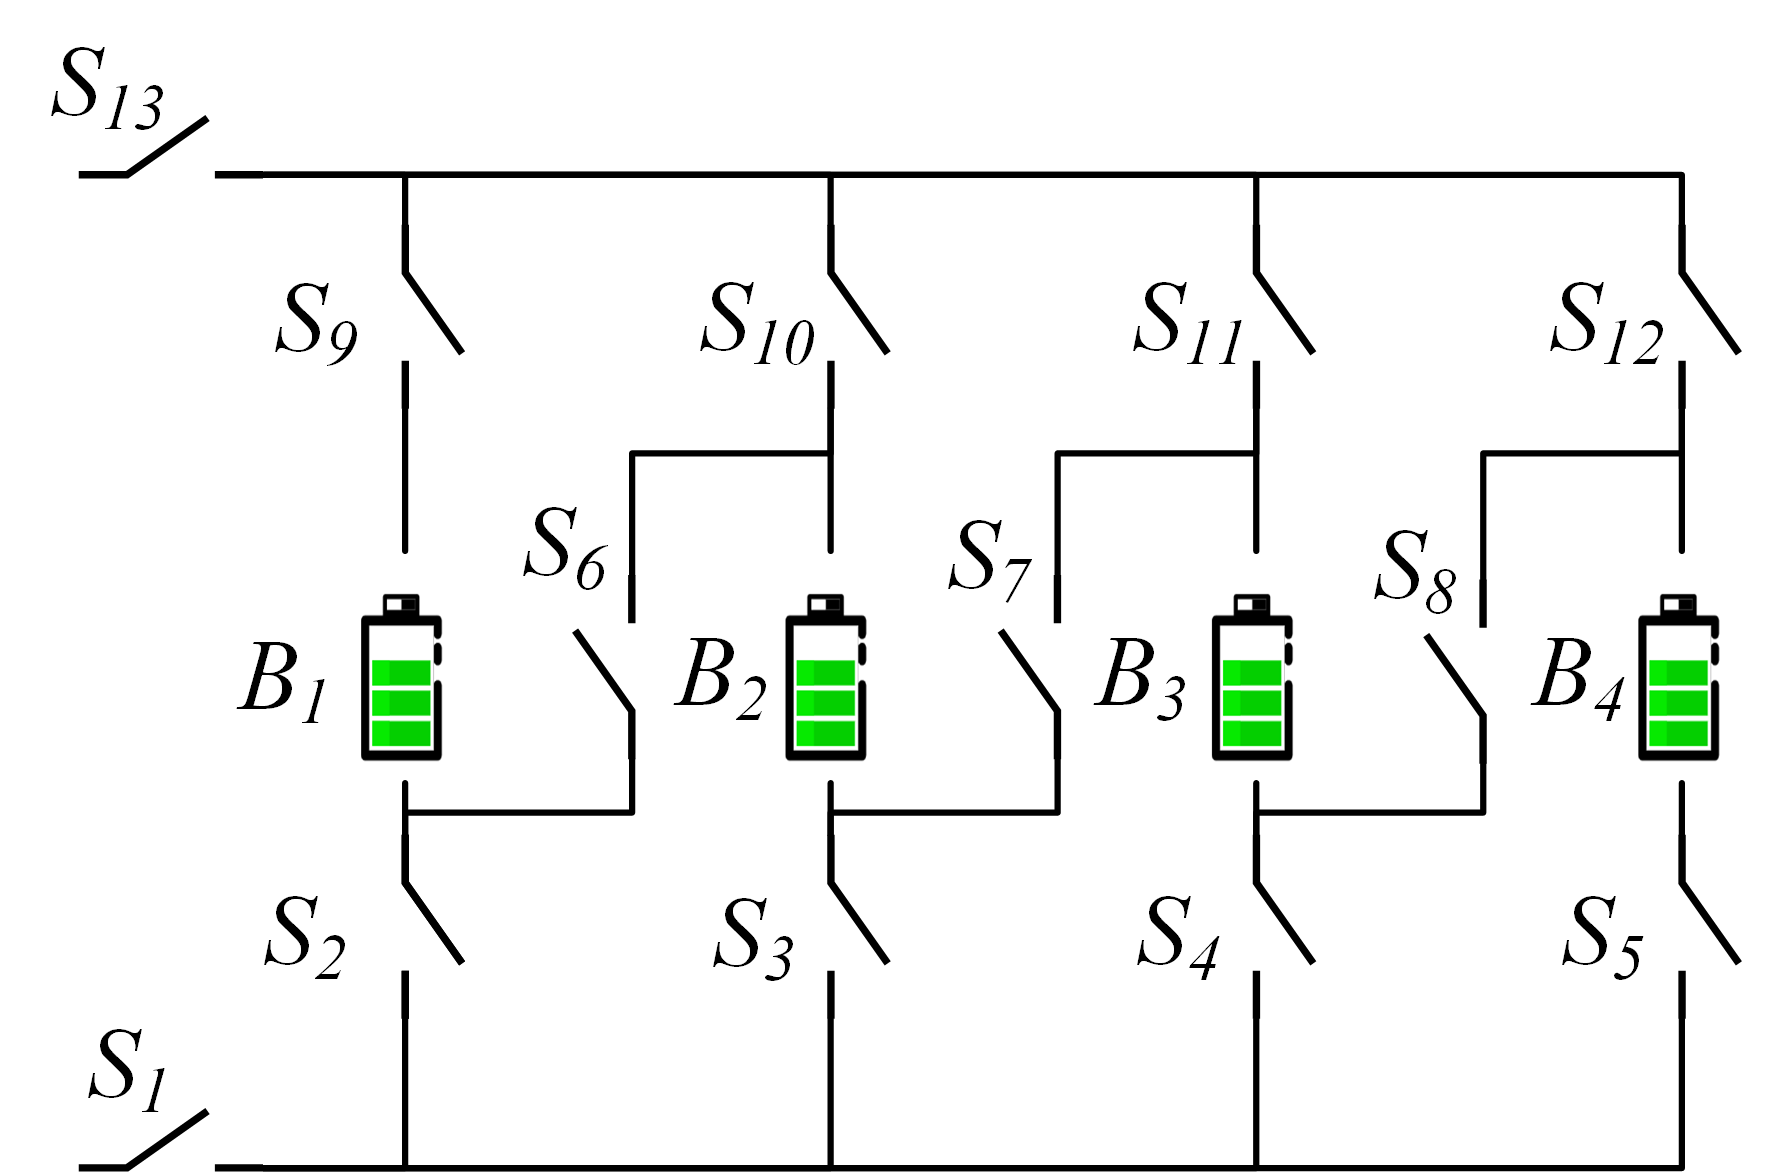
\includegraphics[width=\textwidth]{stru-V-origin.png}
        \caption{}
        \label{fig:study-stru-Visairo}
    \end{subfigure}
    \hspace{0.02\textwidth}
    \begin{subfigure}[b]{0.31\textwidth}
        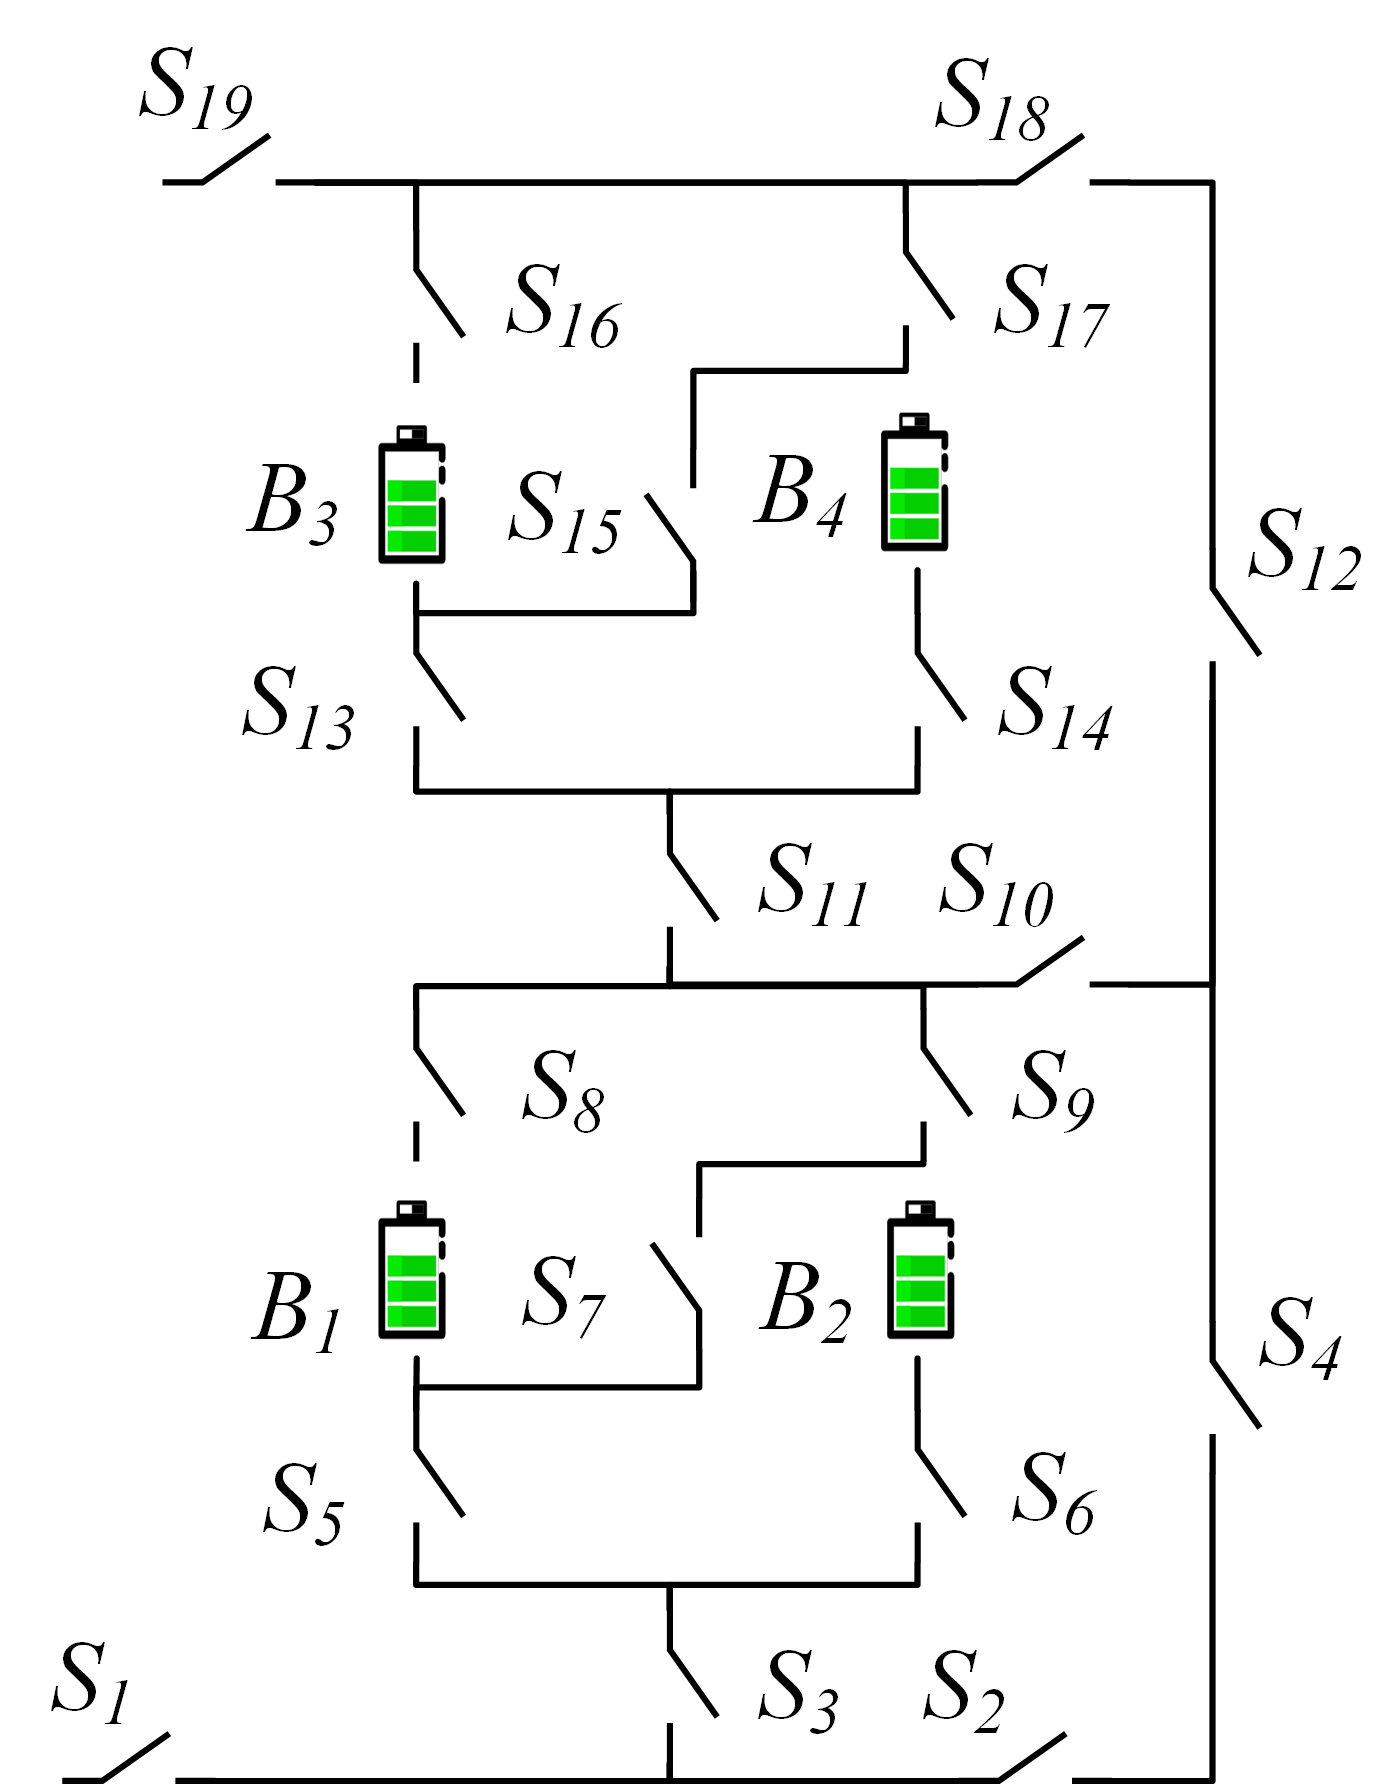
\includegraphics[width=\textwidth]{stru-my-origin.png}
        \caption{}
        \label{fig:study-stru-my}
    \end{subfigure}
    \caption{The four-battery RBS structures proposed by (a) Lawson \cite{lawsonSoftwareConfigurableBattery2012}, (b) Visairo \cite{visairoReconfigurableBatteryPack2008}, and (c) this paper.}
\end{figure}

Currently, two types of RBS structures have been proposed by Visairo et al. \cite{visairoReconfigurableBatteryPack2008} and Lawson et al. \cite{lawsonSoftwareConfigurableBattery2012}, both of which have seen real use. 
The primary goal of Visairo's structure (Fig. \ref{fig:study-stru-Visairo}) is to dynamically adjust the RBS output power. However, the isolation of unhealthy batteries is not sufficiently addressed in their work. 
Lawson et al. designed the RBS structure shown in Fig. \ref{fig:study-stru-Lawson} to isolate batteries. 
Although this structure easily isolates batteries, it cannot dynamically adjust the output current of the RBS. 
Based on the structures of Visairo and Lawson, this paper proposes the structure shown in Fig. \ref{fig:study-stru-my}.
By integrating the Visairo RBS structure into the Lawson RBS structure, the proposed structure not only has the flexibility to switch the batteries between series, parallel, and mixed series-parallel modes but also allows the isolation of highly degraded batteries from the RBS.
These four-battery RBS structures are investigated in the case study, including the scenarios with random isolated batteries.

\subsection{Result}

As shown in Fig. \ref{fig:study-stru-my}, the new RBS structure consists of four batteries and 19 switches. 
Figure \ref{fig:study-dirgraph-my} shows the corresponding directed graph, which is composed of 18 nodes and 43 edges. 
Batteries $B_1$, $B_2$, $B_3$, and $B_4$ are denoted by green directed edges in the graph, and the 19 switches are represented by gray directed edges with bidirectional arrows. 
The external electrical load is treated as a directed edge from the cathode of the RBS (i.e., node 18) to the anode (i.e., node 1), as indicated by the blue directed edge in the graph.
Using Eq. (\ref{eq:weight}) and the Dijkstra algorithm, the SPs of the four batteries in the RBS structure of Fig. \ref{fig:study-stru-my} are highlighted in red in Figs. \ref{fig:sp1} and \ref{fig:sp4}.
Finally, the calculated MACs of the structure in Fig. \ref{fig:study-stru-my} are listed in Tab. \ref{tab:study-results-my} and shown in Fig. \ref{fig:study-results-my}, as obtained by the greedy algorithm \ref{alg:greedy}.
Tab. \ref{tab:study-results-my} contains the states of the switches, the output current $I_o$, the battery current $\bm{I}_b$, and the ratio $\eta$ of the RBS structure with all batteries in good health when the RBS output reaches the MAC.
Fig. \ref{fig:study-results-my} presents the corresponding circuit, with the red highlight indicating that the current is flowing through the respective branches.

\begin{figure}[htbp]
    \centering
    \begin{subfigure}[b]{0.28\textwidth}
        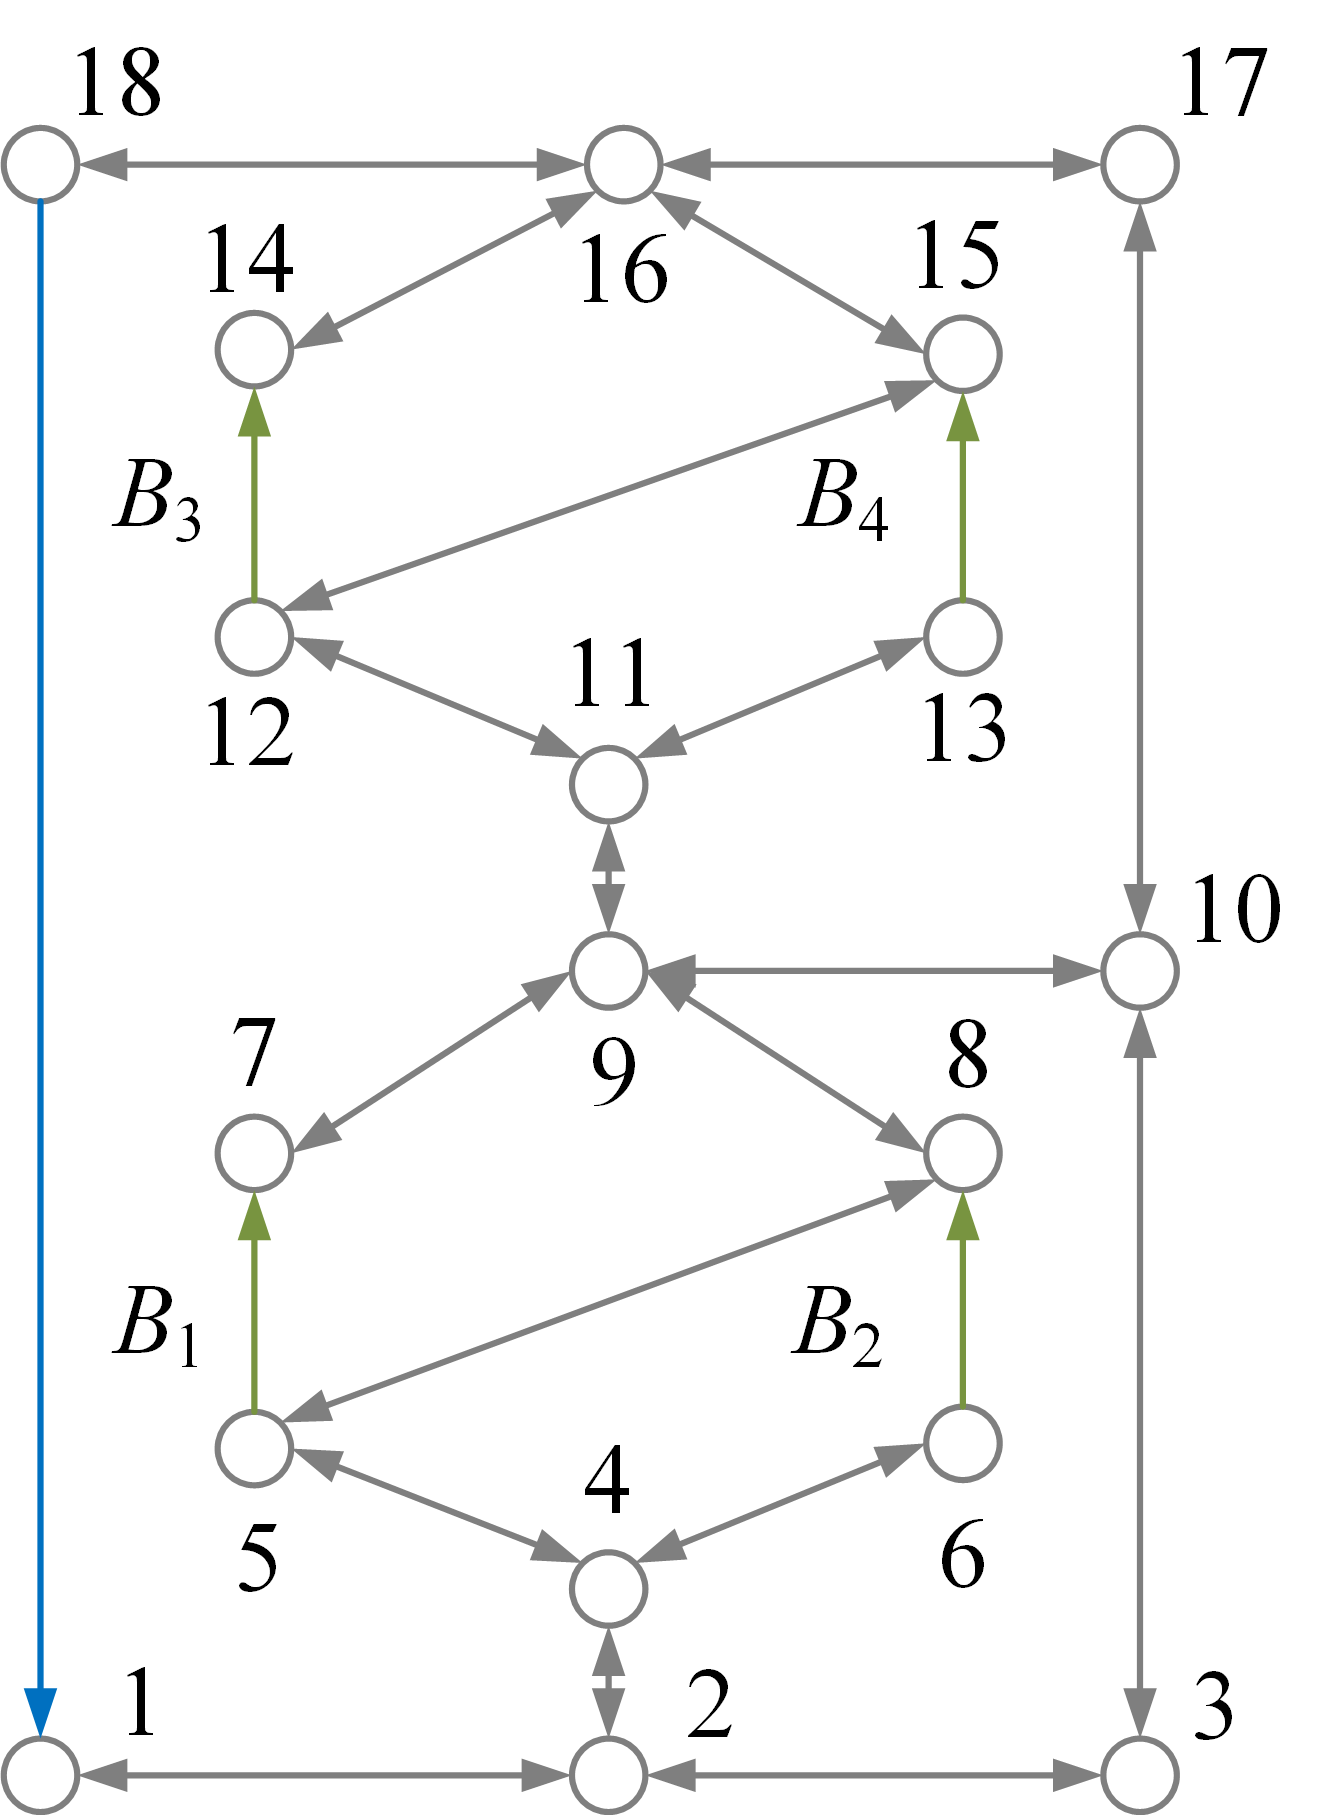
\includegraphics[width=\textwidth]{ef-topo.png}
        \caption{}
        \label{fig:study-dirgraph-my}
    \end{subfigure}
    \hspace{0.05\textwidth}
    \begin{subfigure}[b]{0.28\textwidth}
        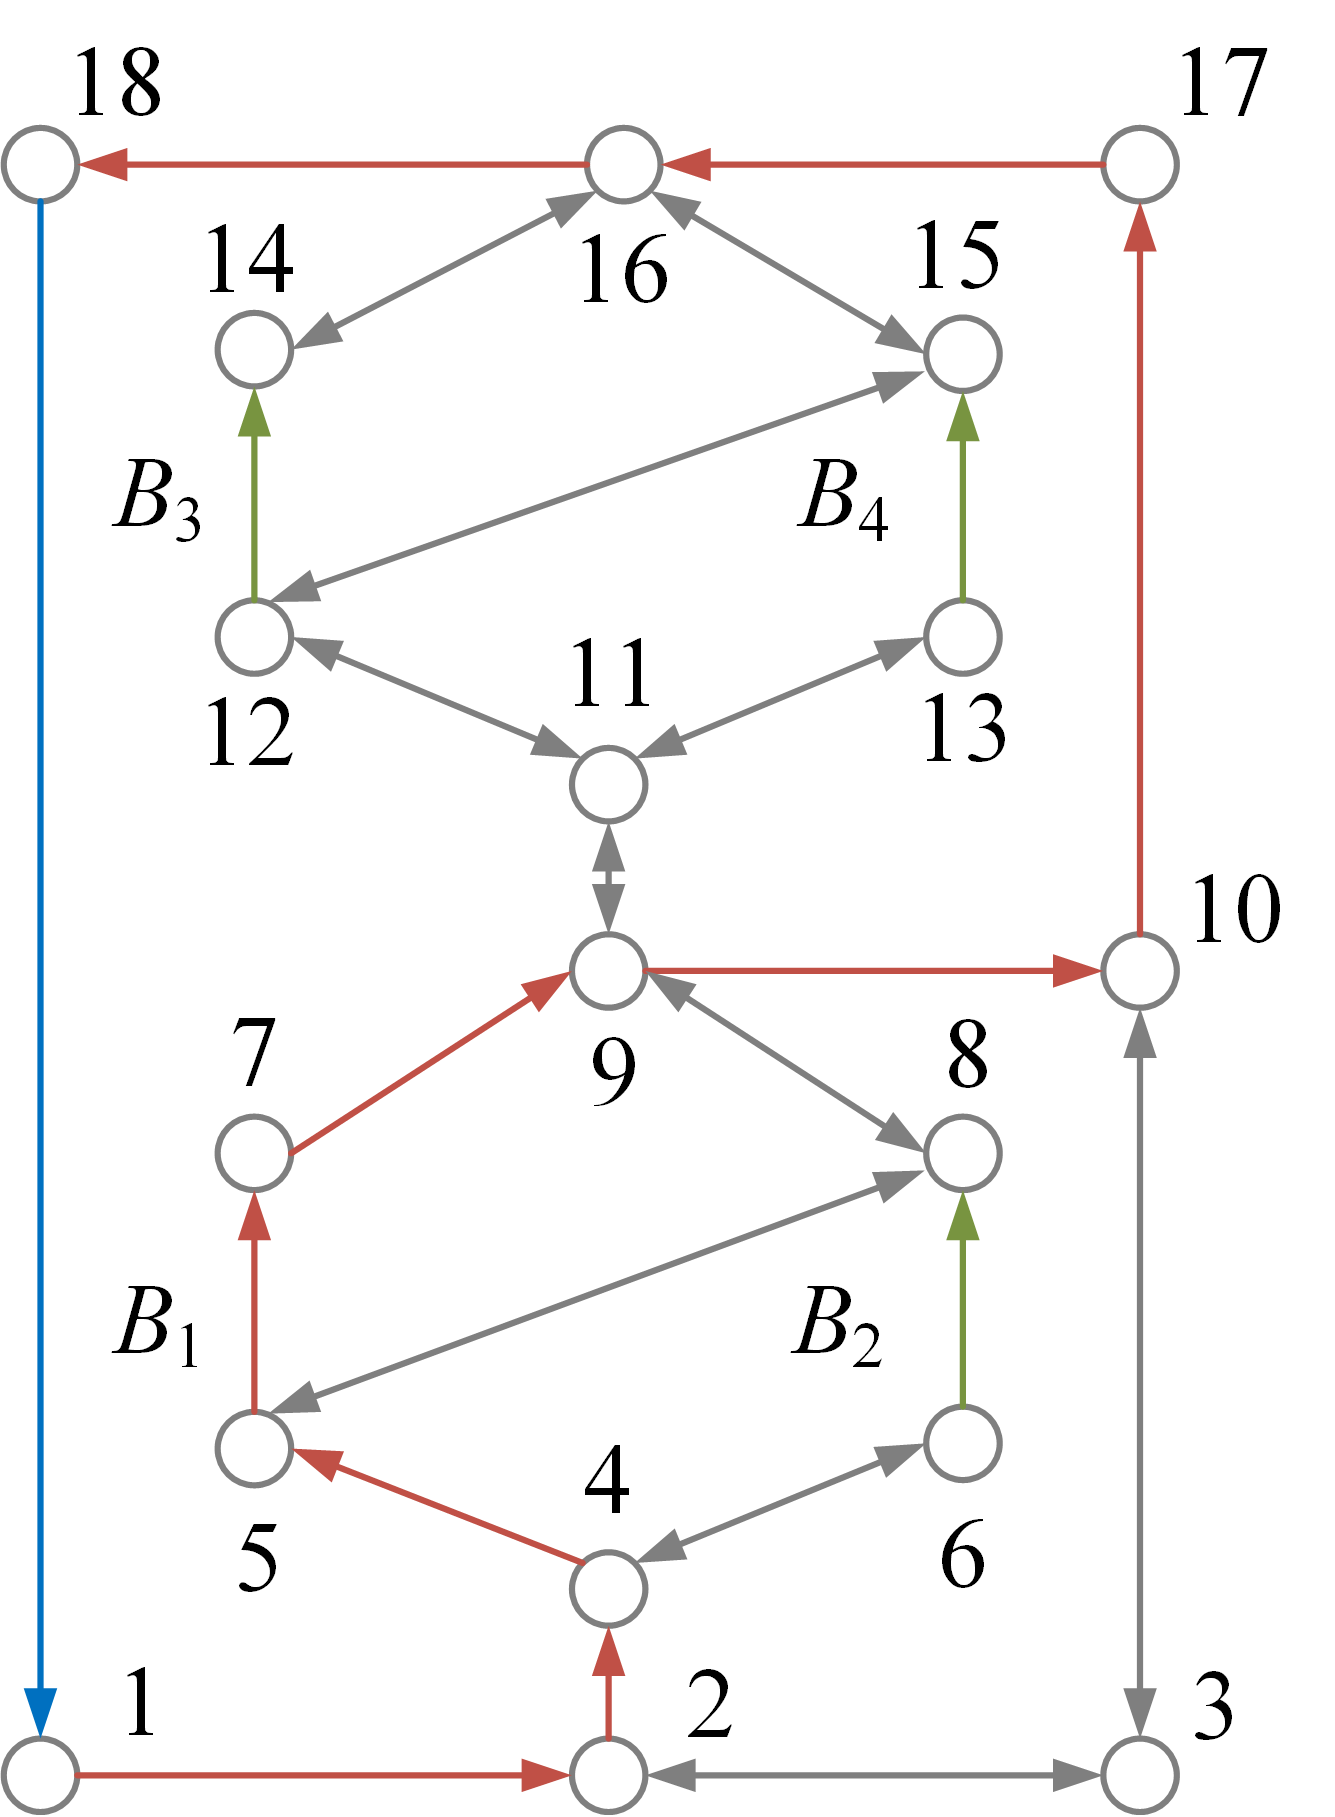
\includegraphics[width=\textwidth]{ef-sp1.png}
        \caption{}
        \label{fig:sp1}
    \end{subfigure}
    \hspace{0.05\textwidth}
    \begin{subfigure}[b]{0.28\textwidth}
        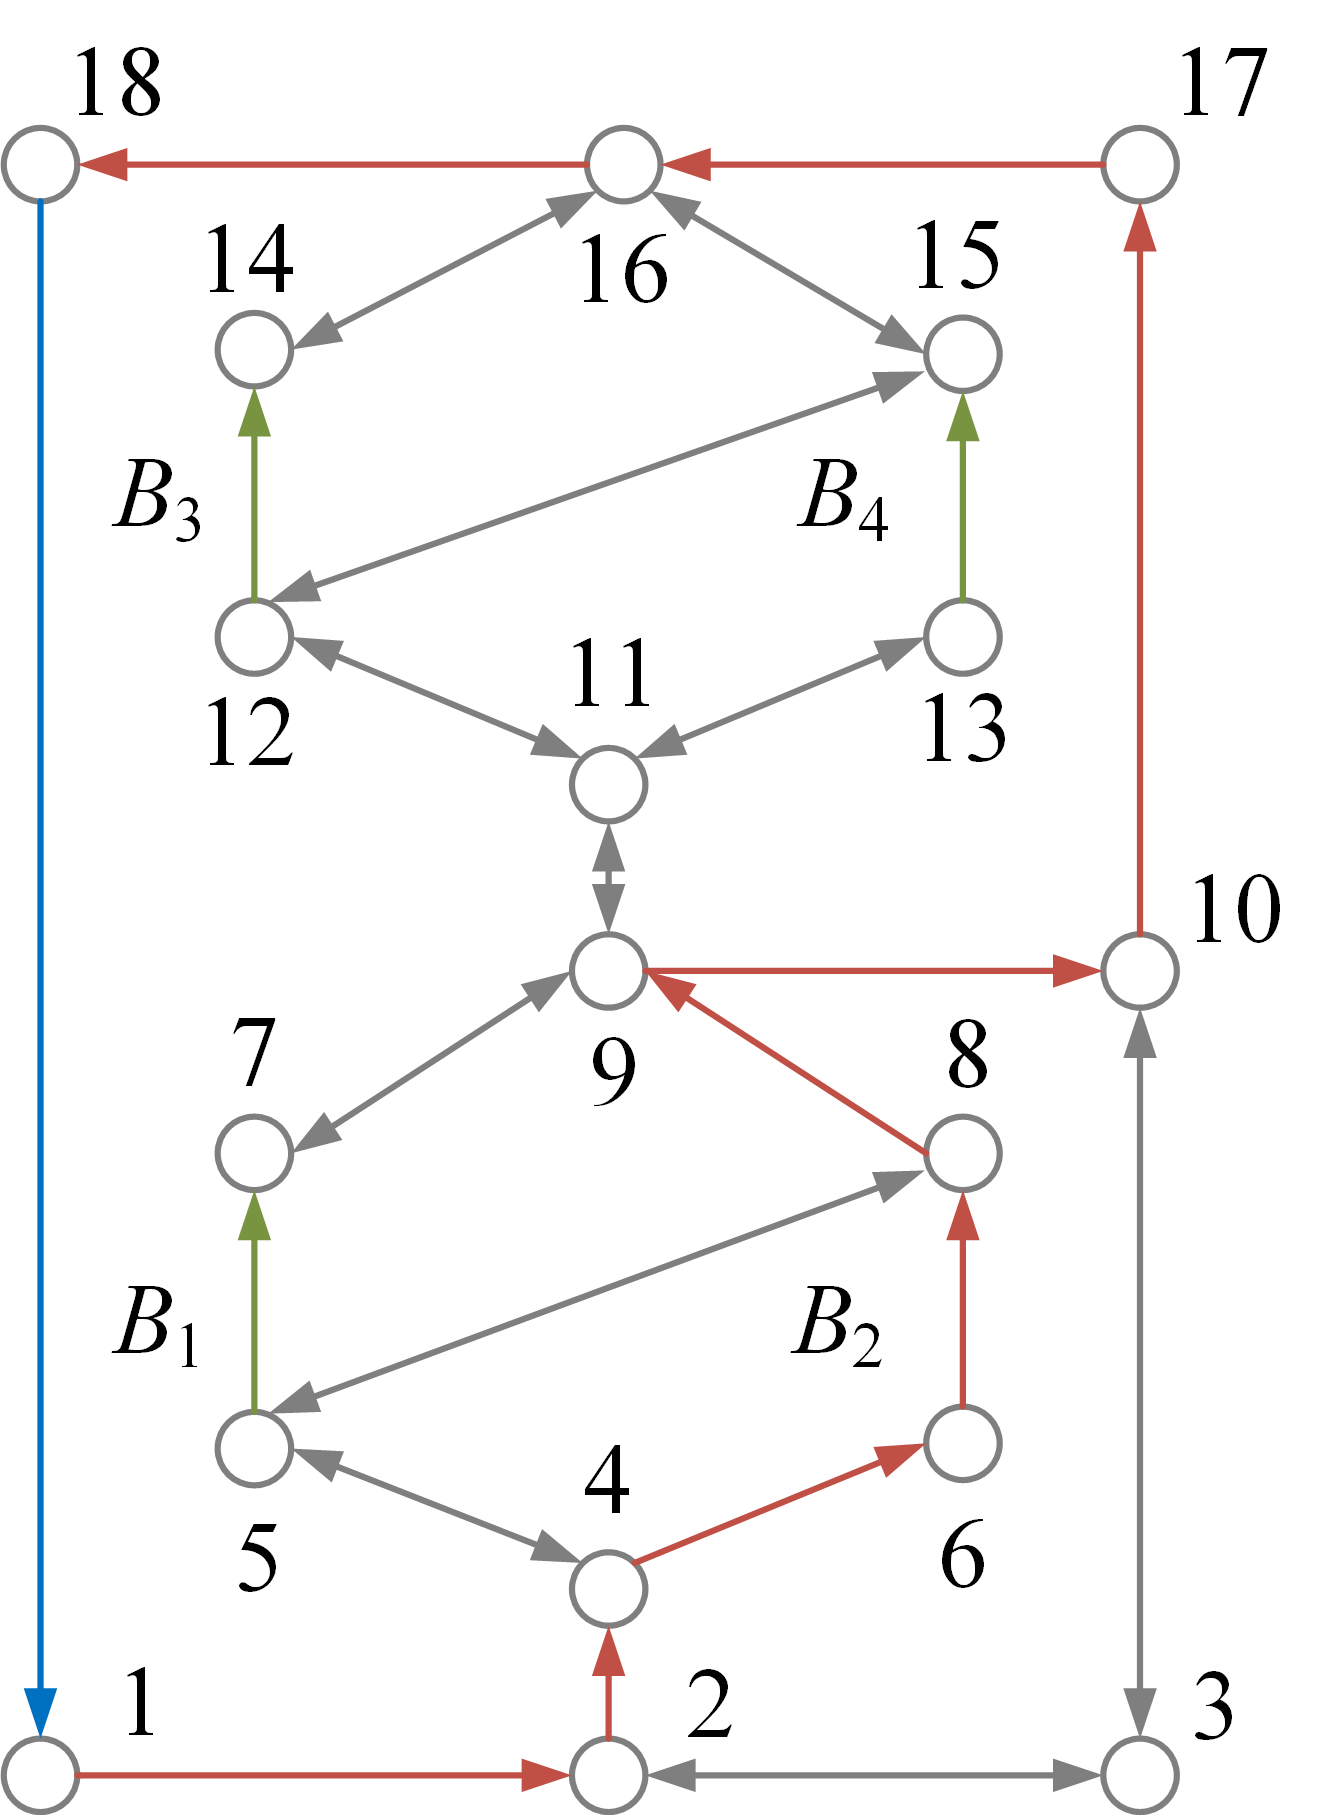
\includegraphics[width=\textwidth]{ef-sp2.png}
        \caption{}
        \label{fig:sp2}
    \end{subfigure}
    \\
    \begin{subfigure}[b]{0.28\textwidth}
        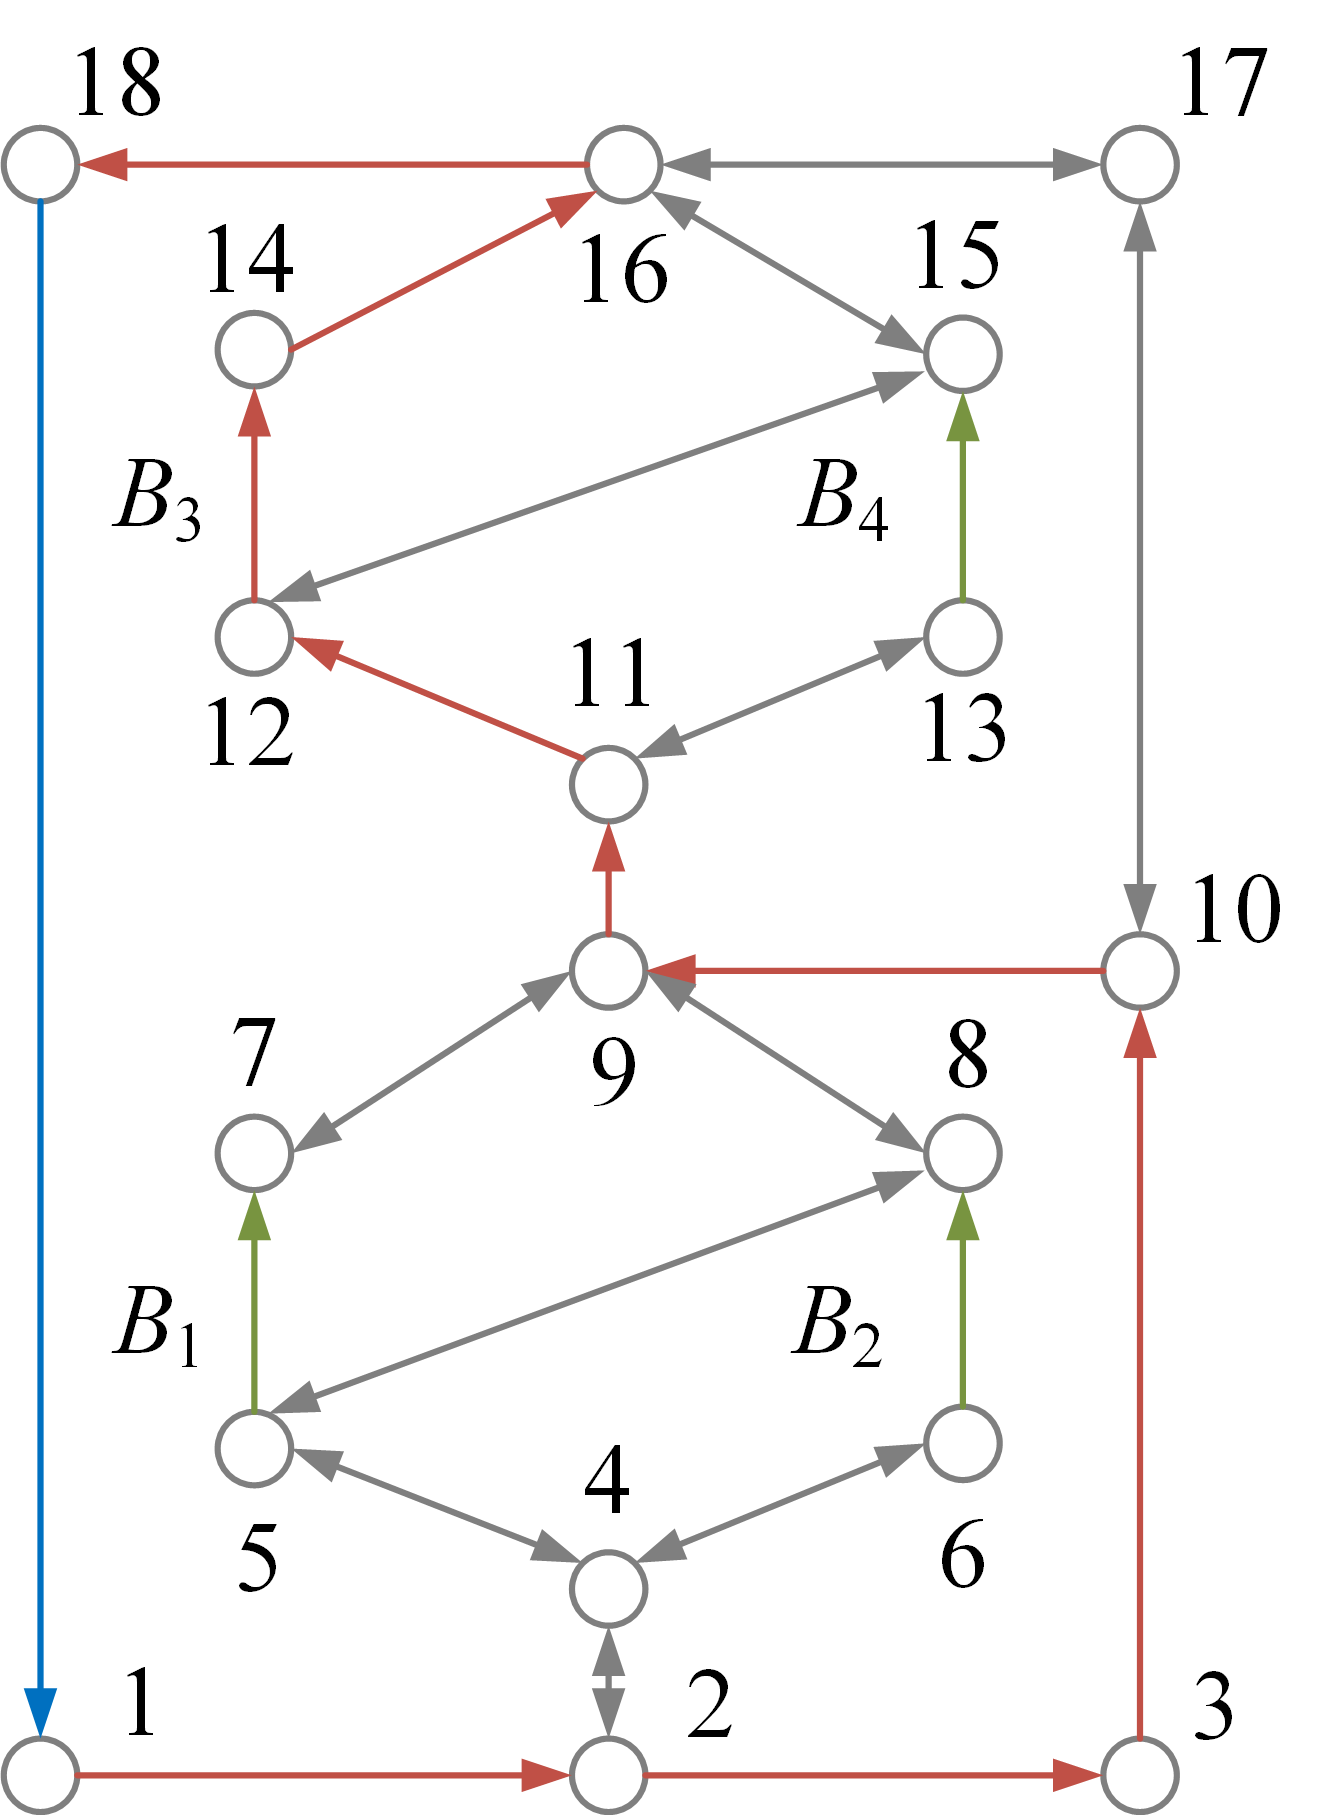
\includegraphics[width=\textwidth]{ef-sp3.png}
        \caption{}
        \label{fig:sp3}
    \end{subfigure}
    \hspace{0.05\textwidth}
    \begin{subfigure}[b]{0.28\textwidth}
        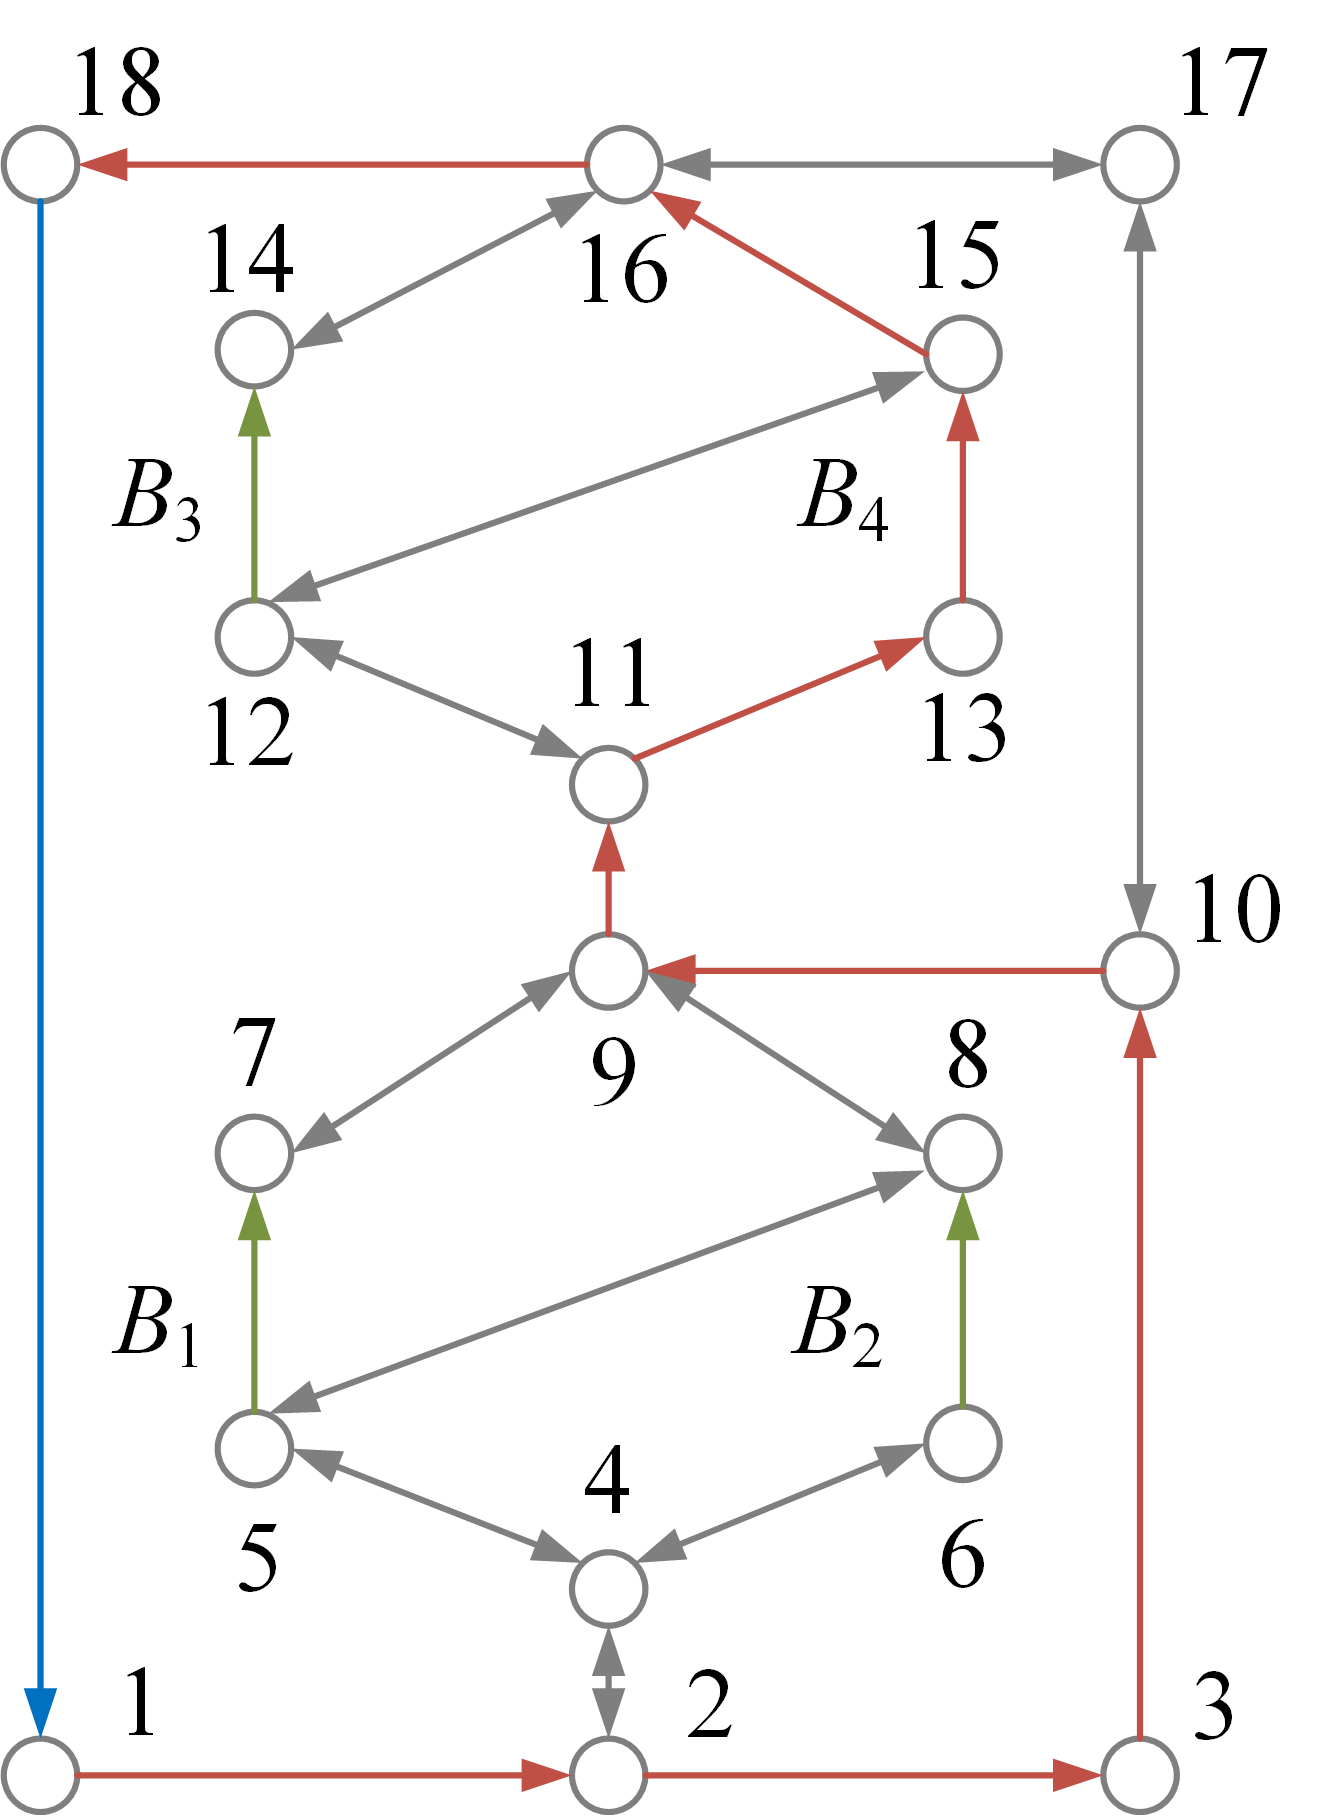
\includegraphics[width=\textwidth]{ef-sp4.png}
        \caption{}
        \label{fig:sp4}
    \end{subfigure}
    \hspace{0.05\textwidth}
    \begin{subfigure}[b]{0.28\textwidth}
        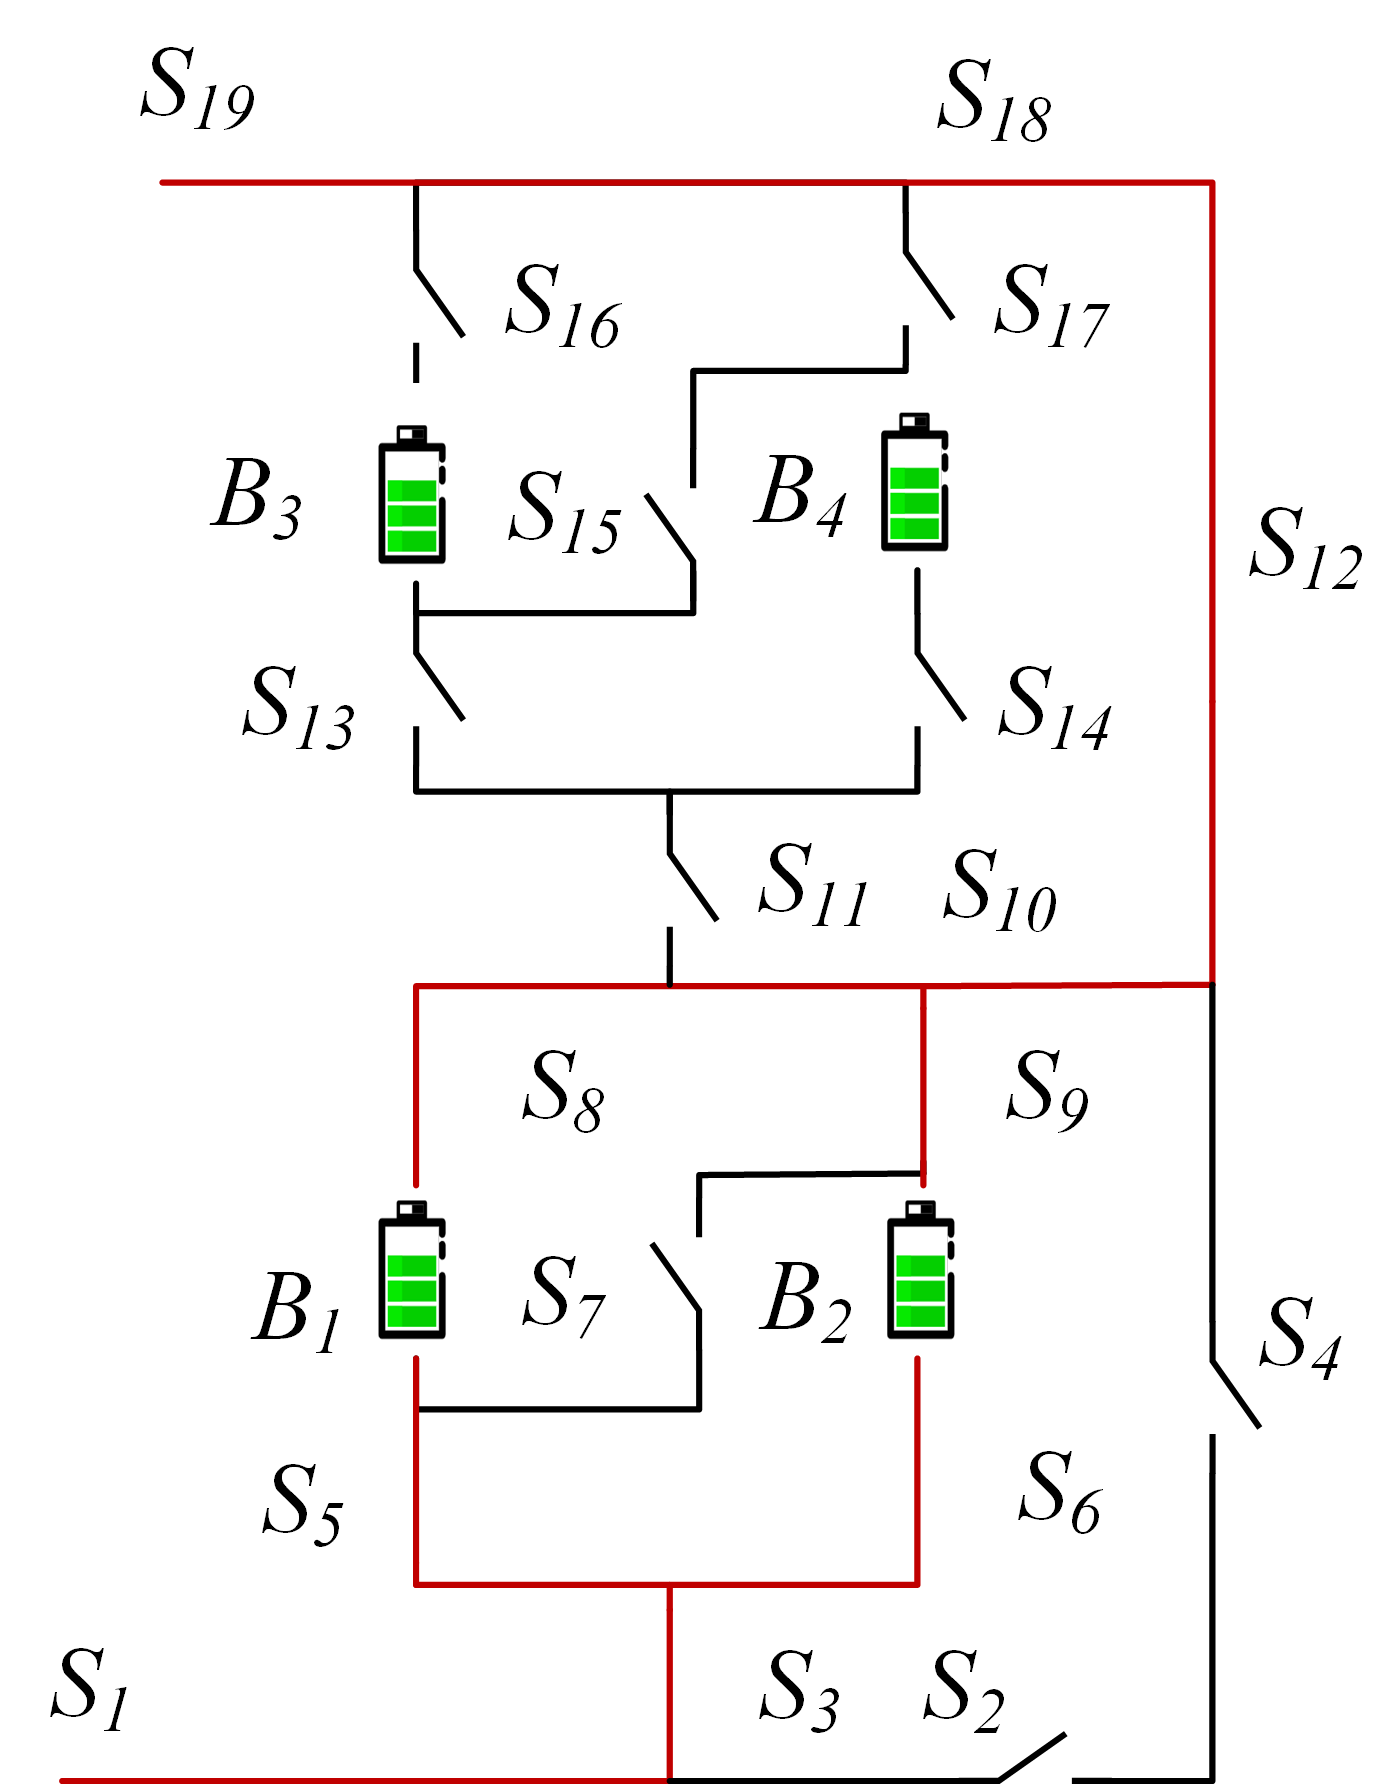
\includegraphics[width=\textwidth]{ef-mac.png}
        \caption{}
        \label{fig:study-results-my}
    \end{subfigure}
    \caption{
        For the RBS structure in Fig. \ref{fig:study-stru-my}, 
        (a) its directed graph 
        and the SPs (highlighted in red) of battery (b) $B_1$, (c) $B_2$, (d) $B_3$, and (e) $B_4$.
        (f) Circuit of RBS with its output reaching the MAC.
        }
    \label{fig:all-results-my}
\end{figure}

\begin{table}[htbp]
  \centering
    \caption{Calculated MAC for four-battery RBS structure in Fig. \ref{fig:study-stru-my}.}
    \begin{tabular}{cc}
    \toprule
        Structure & Figure \ref{fig:study-stru-my} with four batteries and 19 switches  \\
    \midrule
    Switch on & $S_1$,$S_3$,$S_5$,$S_6$,$S_8$,$S_9$,$S_{10}$,$S_{12}$,$S_{18}$,$S_{19}$ \\
    $I_o$ & $2u_b/(2R_o+r_b)$ \\
    $\bm{I}_b$ & $[u_b/(2R_o+r_b),u_b/(2R_o+r_b),0,0]$ \\
    $\max \eta$     & 2 \\
    \bottomrule
    \end{tabular}
  \label{tab:study-results-my}
\end{table}

Similarly, the results of the MAC calculation for the structures in Figs. \ref{fig:study-stru-Lawson} and \ref{fig:study-stru-Visairo} are listed in Tabs. \ref{tab:study-results-Lawson} and  \ref{tab:study-results-Visairo}, respectively.


To verify and compare the results from the greedy algorithm, we also used a brute-force algorithm that iterates through all possible switch states to calculate the MAC of the same three RBSs. 
The final results are the same as the results shown in Tabs. \ref{tab:study-results-my}--\ref{tab:study-results-Visairo}.
The method uses the greedy algorithm to calculate 11, 11, and 1 reconfigured structures for the RBS structure in Figs. \ref{fig:study-stru-my}, \ref{fig:study-stru-Lawson}, and \ref{fig:study-stru-Visairo}, respectively. 
For the same RBS, the method counts all possible switch states, which equates to $2^{19}$, $2^{15}$, and $2^{13}$ structures, respectively.

\begin{table}[htbp]
  \centering
    \caption{MAC Calculating result of the four-battery RBS structure in Fig. \ref{fig:study-stru-Lawson}.}
    \begin{tabular}{cc}
    \toprule
        Structure & Figure \ref{fig:study-stru-Lawson} with 4 batteries and 15 switches  \\
    \midrule
    Switch ON & $S_1$,$S_3$,$S_5$,$S_7$,$S_{10}$,$S_{13}$,$S_{14}$,$S_{15}$ \\
    $I_o$ & $u_b/(R_o+r_b)$ \\
    $\bm{I}_b$ & $[u_b/(R_o+r_b),0,0,0]$ \\
    $\max \eta$     & 1 \\
    \bottomrule
    \end{tabular}
  \label{tab:study-results-Lawson}
\end{table}

\begin{table}[htbp]
  \centering
    \caption{MAC Calculating result of the four-battery RBS structure in Fig. \ref{fig:study-stru-Visairo}.}
    \begin{tabular}{cc}
    \toprule
        Structure & Figure \ref{fig:study-stru-Visairo} with 4 batteries and 13 switches  \\
    \midrule
    Switch ON & $S_1$,$S_2$,$S_3$,$S_4$,$S_5$,$S_9$,$S_{10}$,$S_{11}$,$S_{12}$,$S_{13}$ \\
    $I_o$ & $4u_b/(4R_o+r_b)$ \\
    $\bm{I}_b$ & $[u_b/(4R_o+r_b),u_b/(4R_o+r_b),u_b/(4R_o+r_b),u_b/(4R_o+r_b)]$ \\
    $\max \eta$     & 4 \\
    \bottomrule
    \end{tabular}
  \label{tab:study-results-Visairo}
\end{table}

Furthermore, the RBS with isolated batteries is taken into consideration and calculated. 
The MAC calculation results for the three structures under study, with varying numbers of isolated batteries, are presented in Tab. \ref{tab:isolated_mac}. 
Figs. \ref{fig:my-isolated-1}--\ref{fig:my-isolated-3} illustrate the corresponding switch-control schemes for the new structure proposed in this paper under different conditions of isolated batteries.

\begin{table}[htbp]
    \centering
    \caption{
      Variation of MAC with the number of isolated batteries for different RBS structures, including the structure proposed by Lawson et al., Visairo et al., and the structure proposed in this paper.
      }
      \label{tab:isolated_mac}
      \begin{tabular}{cccc}
      \toprule
      \multirow{2}[4]{*}{Number of isolated batteries} & \multicolumn{3}{c}{$\eta$ of RBS structure} \\
  \cmidrule{2-4}          & This paper  & Visairo  & Lawson  \\
      \midrule
      0     & 2     & 4     & 1 \\
      1     & 2     & 3     & 1 \\
      2     & 2$^{\mathrm{a}}$ or 1$^{\mathrm{b}}$ & 2     & 1 \\
      3     & 1     & 1     & 1 \\
      \bottomrule
      \end{tabular}
      \\
      \footnotesize{$^{\mathrm{a}}$ Isolate two batteries within the same substructure, as shown in Fig. \ref{fig:my-isolated-2b}.}\\
      \footnotesize{$^{\mathrm{b}}$ Isolate one battery in each of the two substructures, as shown in Fig. \ref{fig:my-isolated-2w}.}
  \end{table}
  
  
  \begin{figure}[htbp]
      \centering
      \begin{subfigure}[b]{0.31\textwidth}
          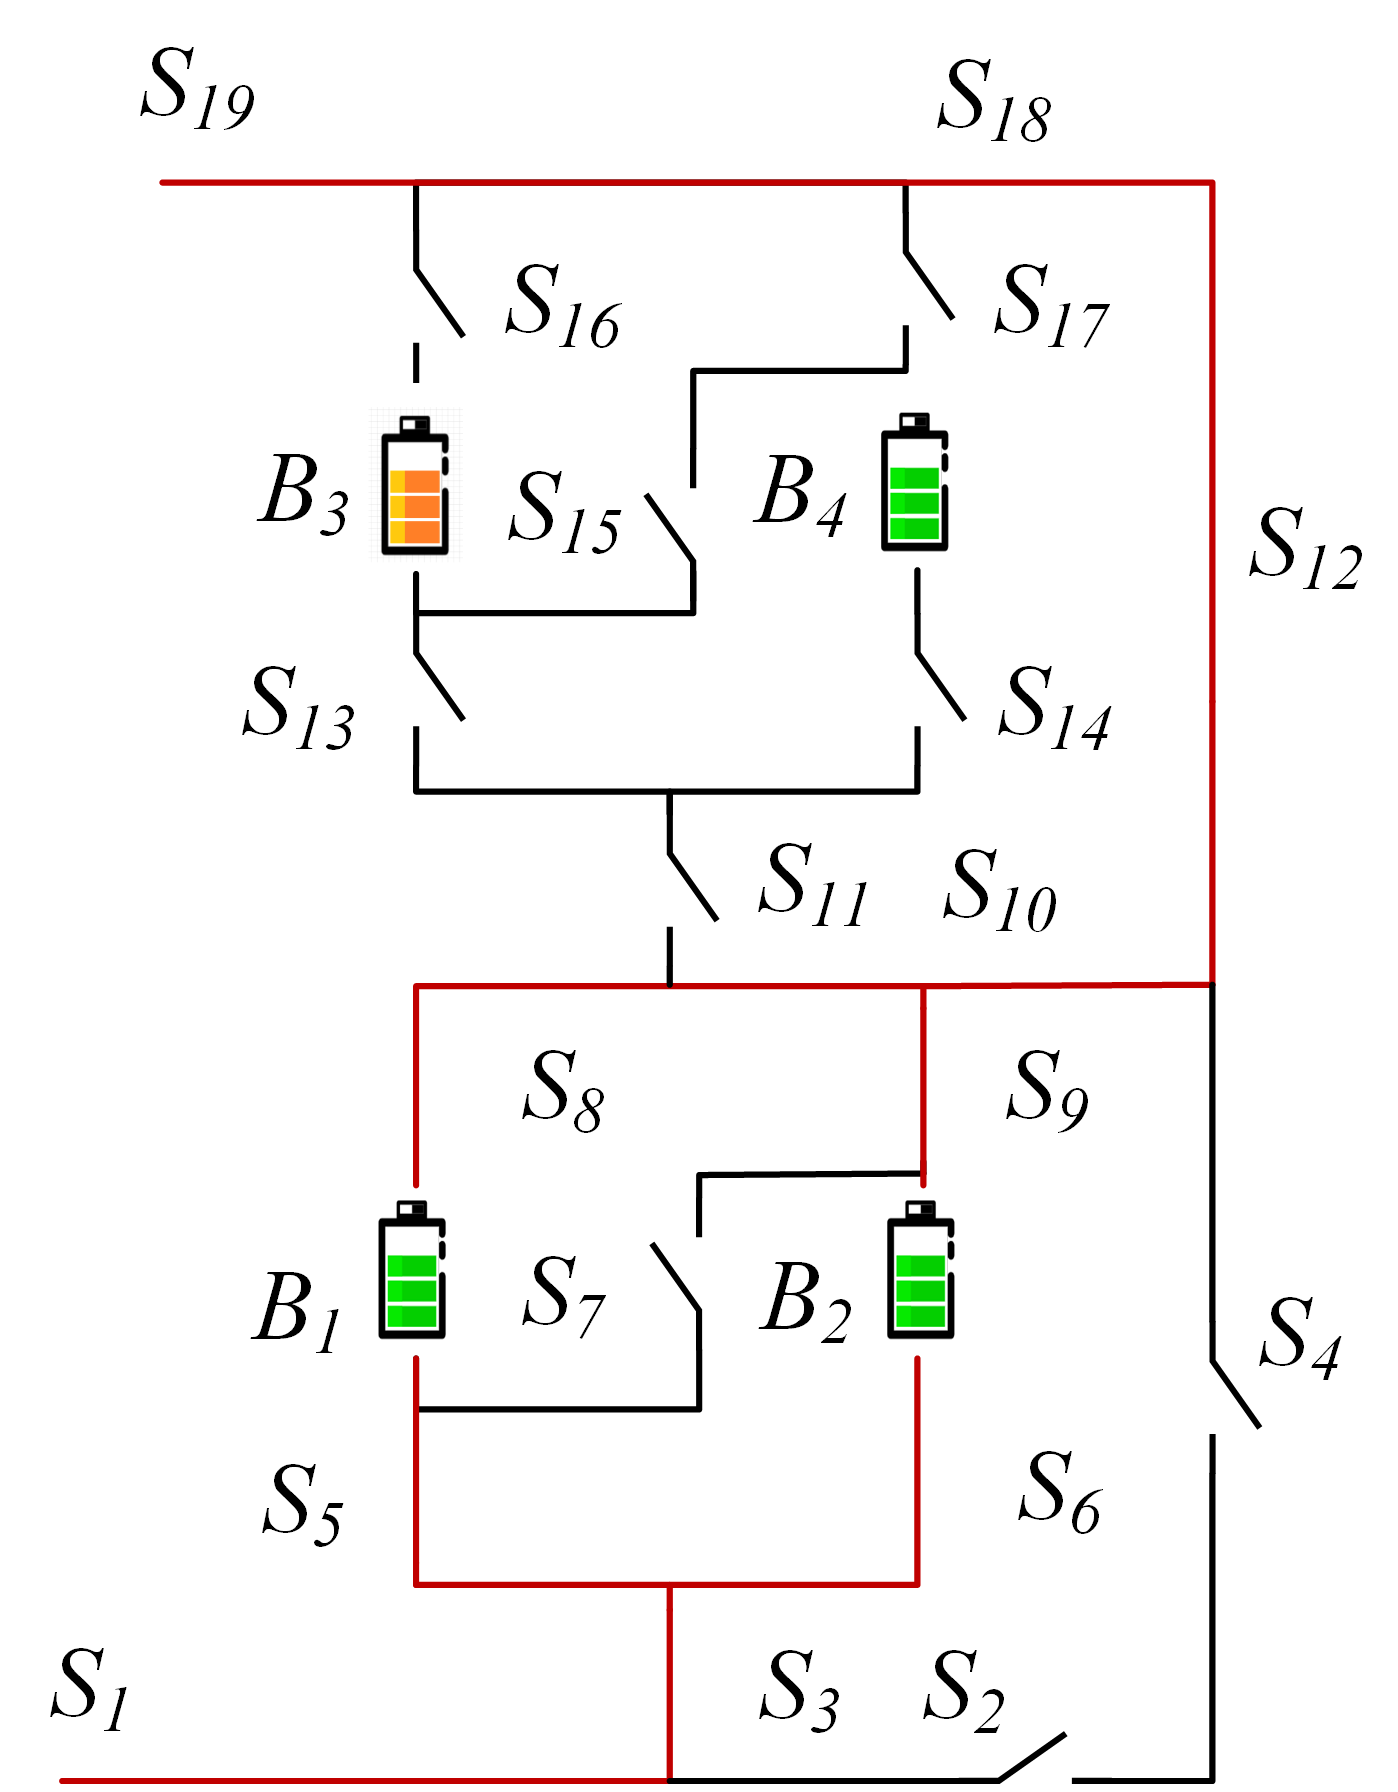
\includegraphics[width=\textwidth]{my-isolated-1.png}
          \caption{}
          \label{fig:my-isolated-1}
      \end{subfigure}
      \hspace{0.02\textwidth}
      \begin{subfigure}[b]{0.31\textwidth}
          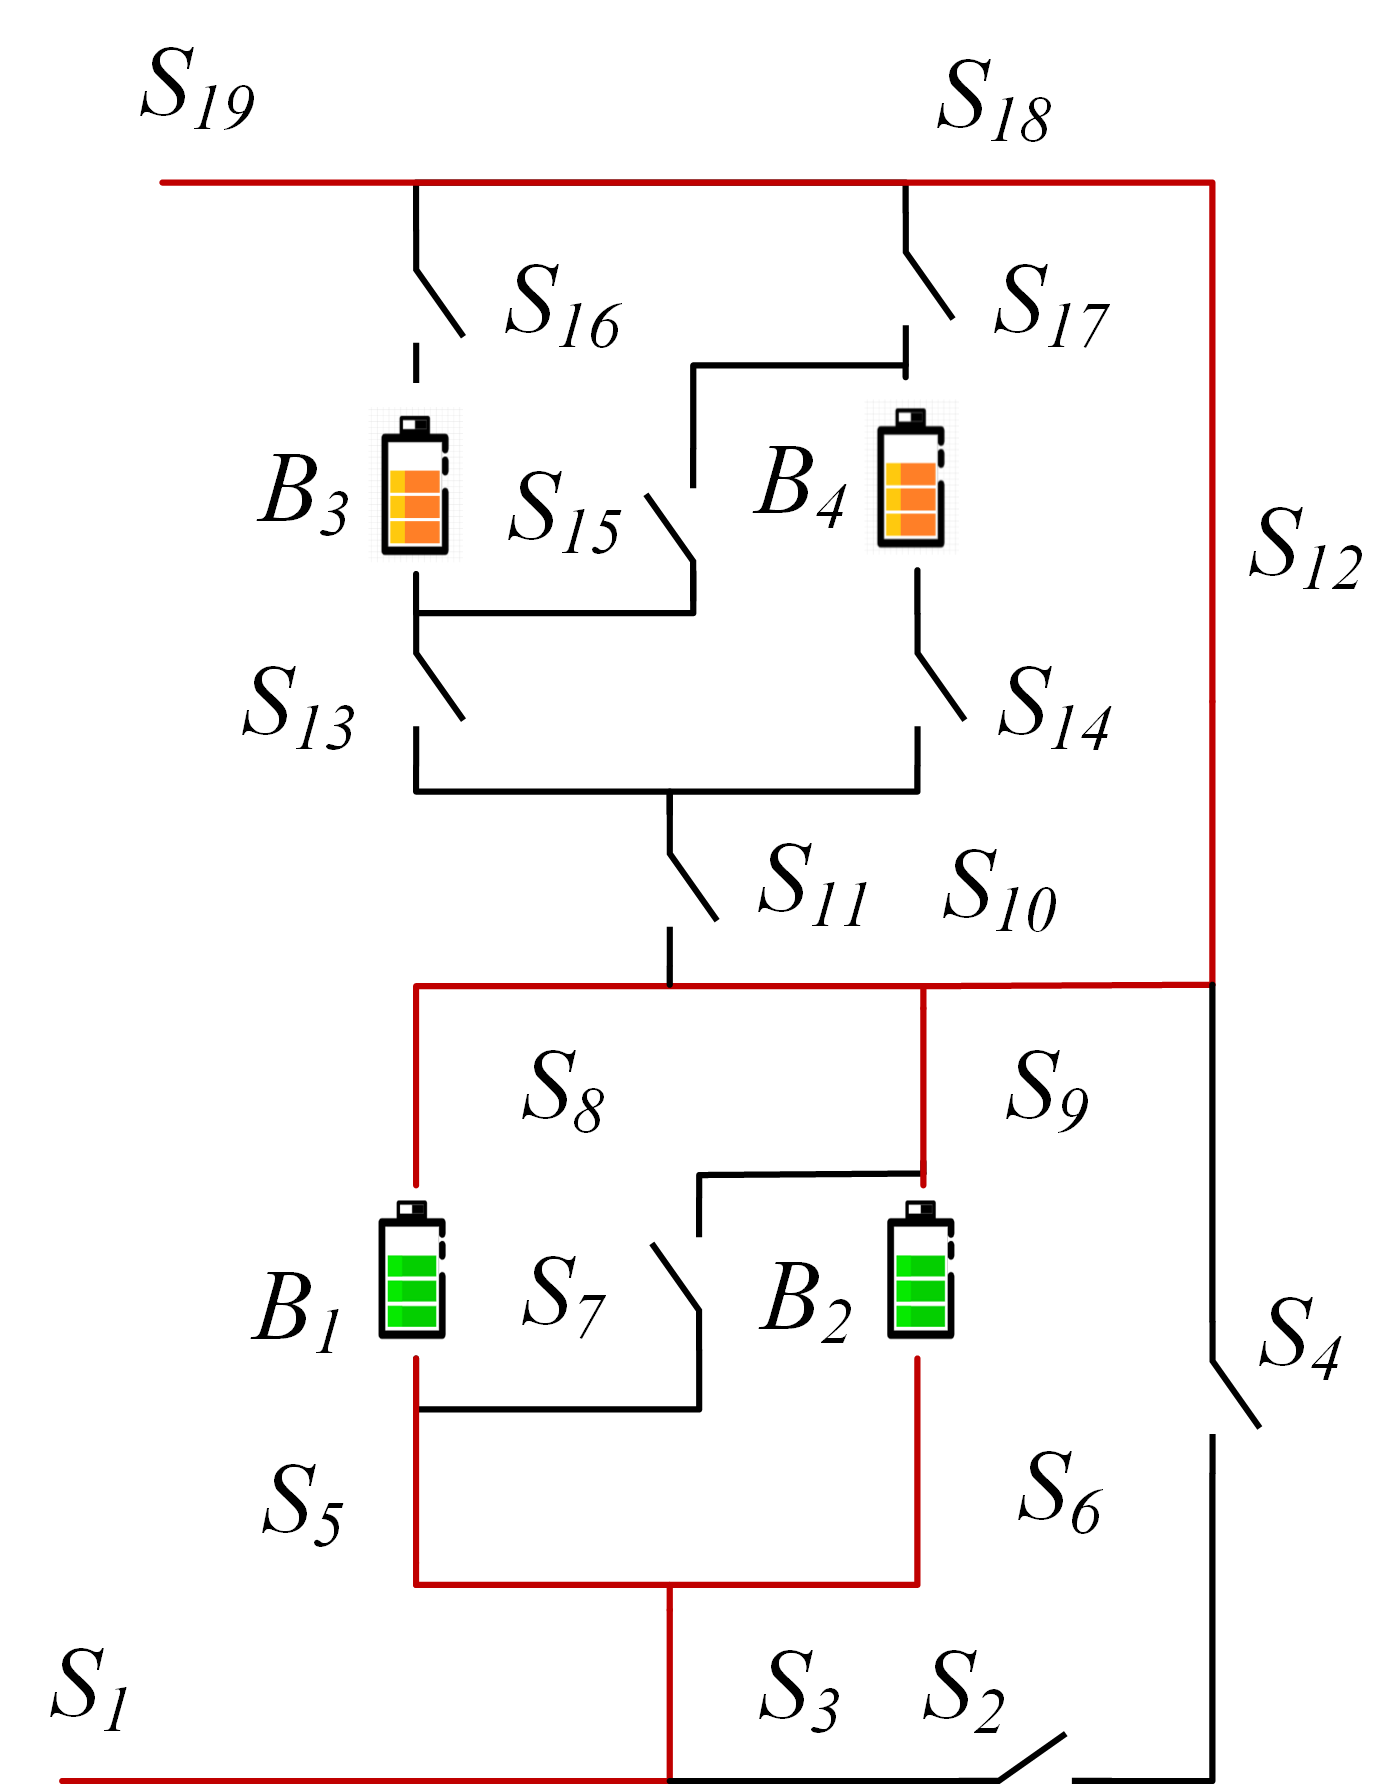
\includegraphics[width=\textwidth]{my-isolated-2b.png}
          \caption{}
          \label{fig:my-isolated-2b}
      \end{subfigure}
      \\
      \begin{subfigure}[b]{0.31\textwidth}
          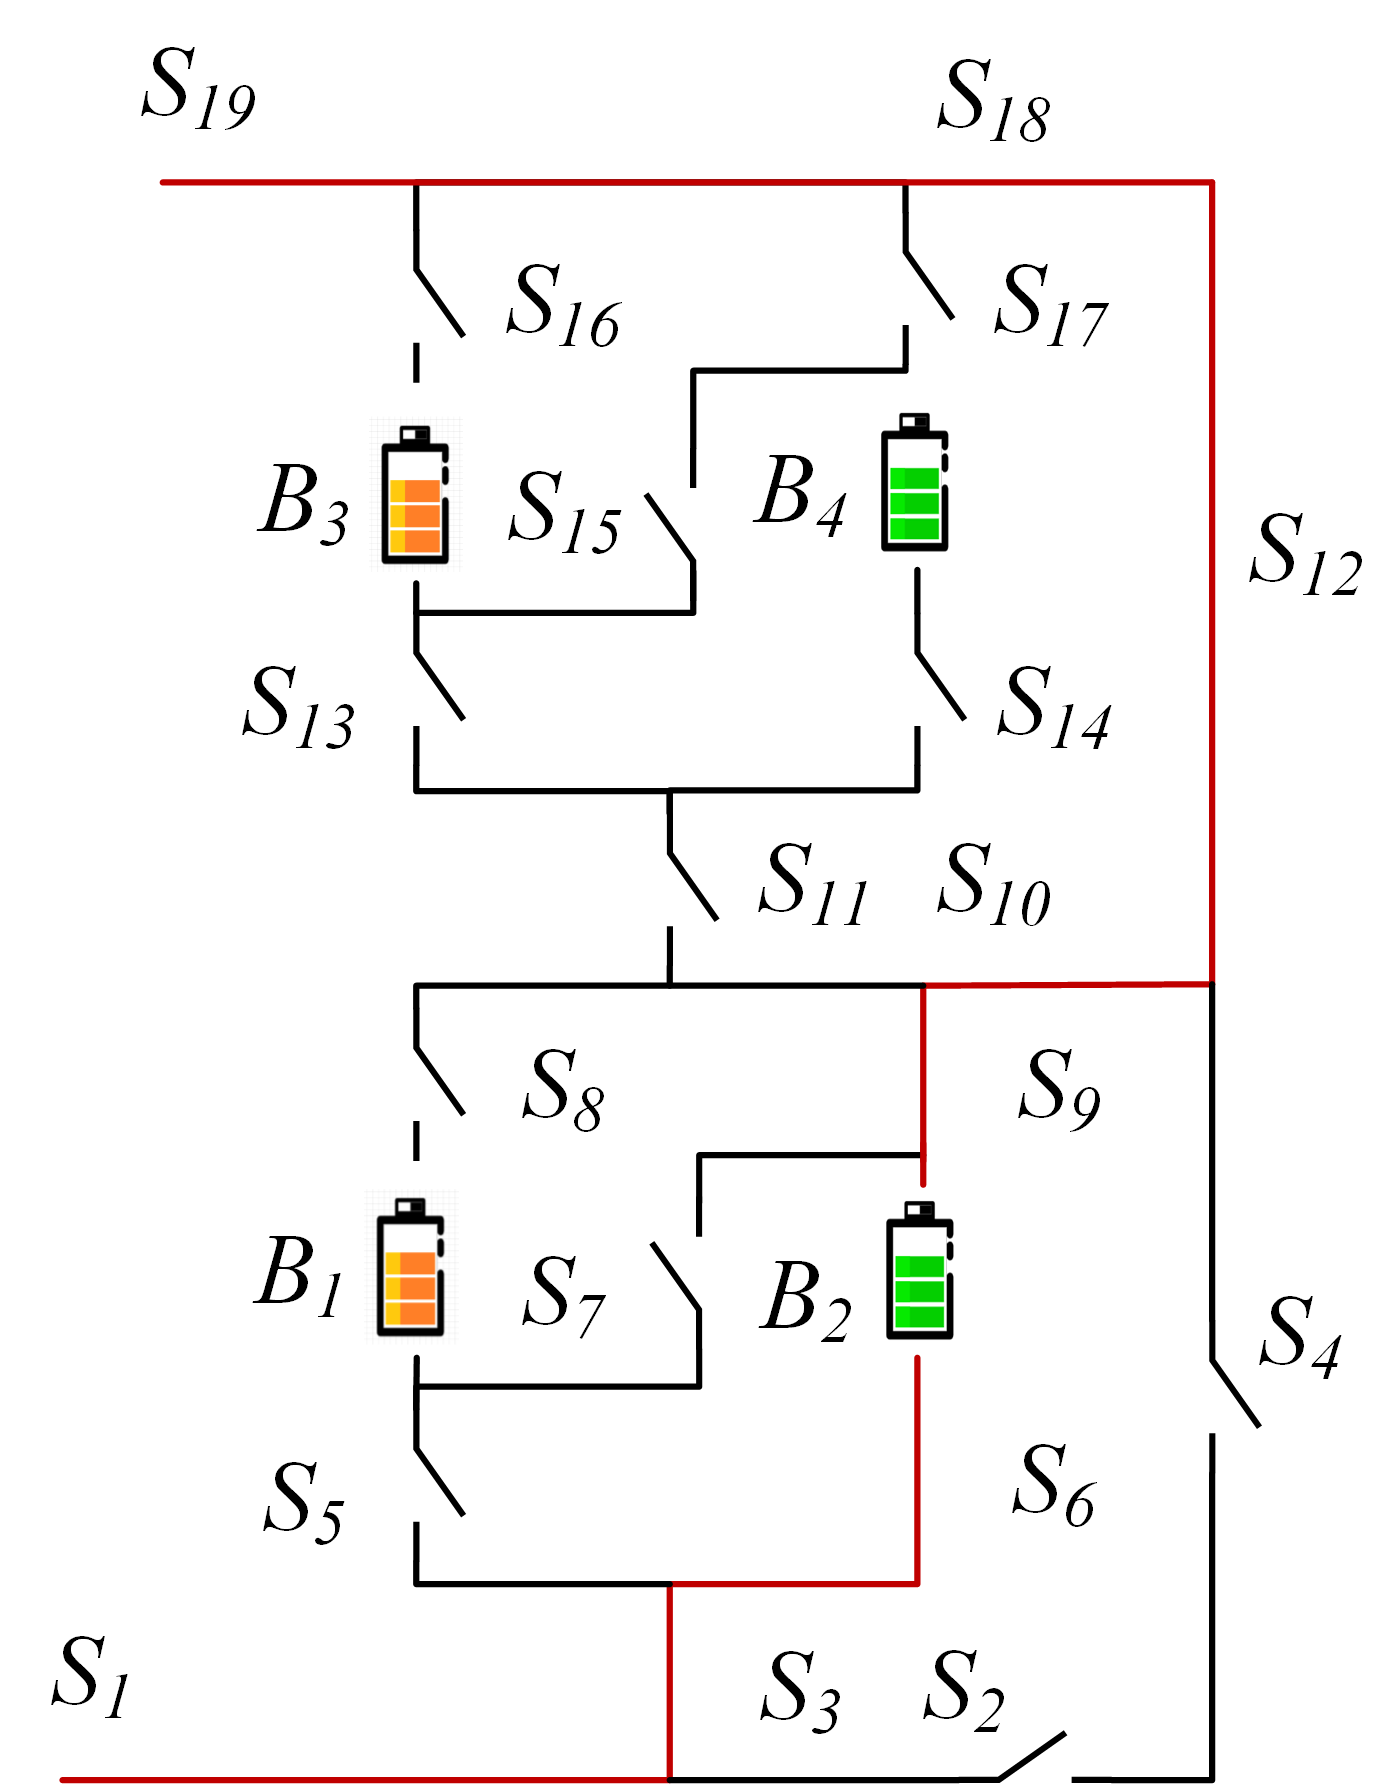
\includegraphics[width=\textwidth]{my-isolated-2w.png}
          \caption{}
          \label{fig:my-isolated-2w}
      \end{subfigure}
      \hspace{0.02\textwidth}
      \begin{subfigure}[b]{0.31\textwidth}
          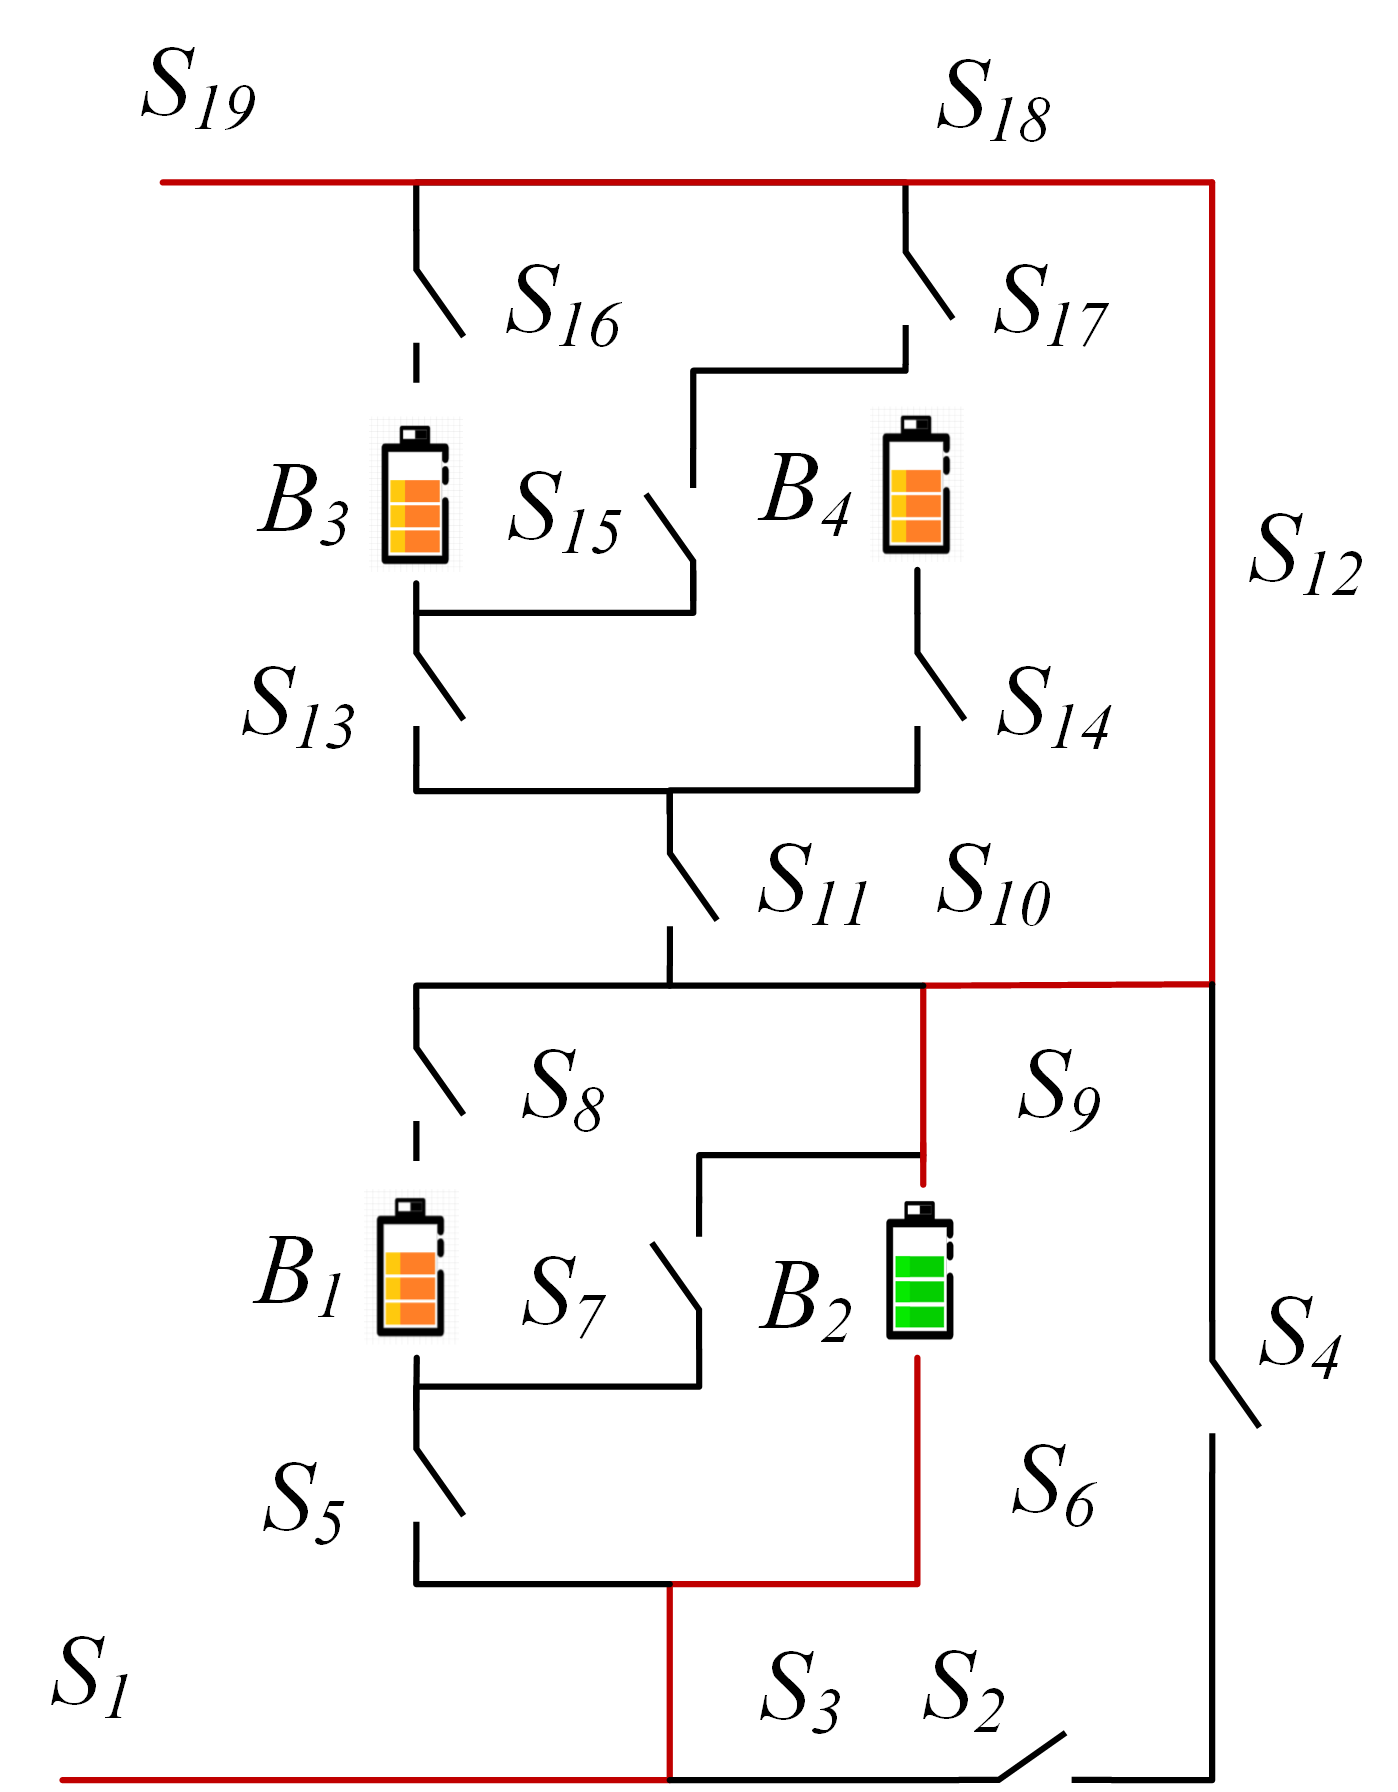
\includegraphics[width=\textwidth]{my-isolated-3.png}
          \caption{}
          \label{fig:my-isolated-3}
      \end{subfigure}
      \caption{
          Circuit states of MACs when isolating (a) one, (b) two (best case), (c) two (worst case), and (d) three batteries for the structure in Fig. \ref{fig:study-stru-my}.
          }
  \end{figure}

\subsection{Discussion}

Consider first the results shown in Fig. \ref{fig:study-results-my} and listed in Tab. \ref{tab:study-results-my}.
When $B_1$ and $B_2$ or $B_3$ and $B_4$ are connected in parallel, the RBS outputs the maximum current, which is $\eta=2$ (i.e., twice the current output of a single battery in the RBS). 
Adding more batteries to the main circuit only forms a series structure and does not improve the MAC. 
Therefore, the state of the switches given in Tab. \ref{tab:study-results-my} maximizes the RBS output current.
The brute-force method, which go through all possible switch states, also gives the same result.


The literature contains no report on an algorithm for calculating the MAC of an RBS.
The brute-force algorithm, which goes through all possible switch states, is the most straightforward way to determine the MAC and is used as a benchmark for the proposed greedy algorithm.
If an RBS has $N_b$ batteries and $N_s$ switches and the corresponding directed graph has $N$ nodes,  $2^{N_s}$ iterations are required to traverse all reconfigured structures.
Calculating each reconfigured structure using Eqs. (\ref{eq:I_o})--(\ref{eq:eta}) requires matrix inversion and matrix multiplication, which has a time complexity of $O(N^3+2N^2N_b+N^2N_s+NN^2_b)$.
Therefore, the time complexity of the brute-force algorithm is $O\bm((N^3+2N^2N_b+N^2N_s+NN^2_b)2^{N_s}\bm)$.
The greedy algorithm proposed in this paper requires  that SP be found for each battery, which requires $N_b$ iterations.
Each SP can be obtained by several applications of Dijkstra's algorithms.
Therefore, the total time complexity for calculating all SPs is $O\bm(N_b(N_b+2N_s)\log_{10} N\bm)$.
According to  Appendix \ref{alg:greedy}, the RBS can reconfigure $C^{N_{\text{set}}}_{N_b}$ structures by selecting $N_{\text{set}}$ batteries from $N_b$ batteries, which gives $\sum^{N_b}_{N_{\text{set}}=1}C^{N_{\text{set}}}_{N_b}/N_b \approx 2^{N_b} N_b^{-1}$ on average.
Thus, with the bisection method, the time complexity of the greedy algorithm is $O\bm((N^3+2N^2N_b+N^2N_s+NN^2_b) 2^{N_b} N_b^{-1} \log_{10} N_b+N_b(N_b+2N_s)\log_{10} N\bm)$.
Based on currently proposed RBS structures \cite{ciNovelDesignAdaptive2007,alahmadBatterySwitchArray2008,kimDependableEfficientScalable2010b,kimBalancedReconfigurationStorage2011a,taesickimSeriesconnectedSelfreconfigurableMulticell2012a,6843711}, the number $N_b$ of batteries, $N_s$ of switches, and $N$ of nodes are quantitatively related as follows: $N_s \approx (3\text{--} 5)N_b$, $N \approx N_s$. 
After simplifying, the time complexity of the method with greedy algorithm is $O(2^{N_b}N_s^2\log_{10} N_b)$, while it is $O(2^{N_s}N_s^3)$ for the method with brute force algorithm.
Therefore, as the RBS grows, especially in the number of switches, the greedy algorithm gains an advantage over the brute-force algorithm.
This is confirmed by the number of structures required to determine the MAC in the previous section. 
Compared with the brute-force algorithm, the method based on the greedy algorithm is 3\,000 to 48\,000 times more efficient, which is theoretically $N_s 2^{N_s - N_b} \log_{10} N_b$ times according to the above time-complexity analysis.
This benefits from two key points:
\begin{enumerate}
\item[(1)] The SPs guide the RBS to reconfigure reasonable structures rather than blindly going through all possible structures. This reduces the complexity from $2^{N_s}$ to $2^{N_b}$, which is the main reason for the improvement in efficiency.
\item[(2)] The bisection method further accelerates this process, reducing the complexity from $2^{N_b}$ to $2^{N_b} N_B^{-1} \log_{10} N_b$.
\end{enumerate}
However, the greedy algorithm proposed in this paper still contains exponential terms in the time complexity, which means it may not be able to handle extremely large RBS structures having large $N_b$.



Note that $\eta$ is used as the objective function instead of $I_o$ in solving for the MAC. 
This choice makes the resulting MAC more reasonable. 
As shown in Tab. \ref{tab:study-results-my}, $I_o$ and $\bm{I}_b$ are functions of $R_o$, $u_b$, and $r_b$. 
However, when $I_o$ is used as the objective function, even for the same RBS structure, the MAC solution and corresponding switch states could change due to different external electrical appliances.
This would increase the difficulty and uncertainty of designing the RBS structure. 
To eliminate this problem, the ratio $\eta=I_o/\max\bm{I}_b$ is adopted as the objective function in our research.
Recall that $\eta$ reflects only the structure's ability to output current, rather than the actual current outputing by the battery system.
Assuming that the MAC of batteries in the RBS is $I_m$, the maximum output current of the RBS structure can be calculated as $\eta I_m$ by determining the value of $\eta$ for the structure. 


The method proposed in this paper facilitates the design of RBSs in the following ways:
Most currently proposed RBS structures \cite{ciNovelDesignAdaptive2007,alahmadBatterySwitchArray2008,kimDependableEfficientScalable2010b,kimBalancedReconfigurationStorage2011a,taesickimSeriesconnectedSelfreconfigurableMulticell2012a,6843711} have simple topological characteristics, so calculating the MACs is relatively straightforward, even intuitive.
However, these simple structures do not always fully satisfy the requirements of complex applications, such as dynamically adapting the circuit to variable and random operating conditions or actively equalizing differences between batteries in the RBS.
Moreover, isolating the batteries disrupts the original regularity and symmetry of the topology, which complicates the otherwise simple structure, and the maximum output current of the system becomes more challenging to obtain.
In contrast, the proposed method calculates the MAC of arbitrary RBS structures, notably the complex and flexible RBS structures.


To illustrate this point, the MACs of three RBS structures mentioned above are calculated after isolating one or more of the batteries, as shown in Tab. \ref{tab:isolated_mac}. 
Specifically, for the structure presented in Fig. \ref{fig:study-stru-my}, the corresponding circuit states for the MACs when isolating one to three batteries are depicted in Figs. \ref{fig:my-isolated-1}--\ref{fig:my-isolated-3}. 
This structure has two cases in which two batteries are isolated: 
one is to isolate two batteries within the same substructure (Fig. \ref{fig:my-isolated-2b}), in which case $\eta=2$; the other is to isolate one battery in each of the two substructures (Fig. \ref{fig:my-isolated-2w}), in which case $\eta=1$. 
The results in Figs. \ref{fig:my-isolated-1}--\ref{fig:my-isolated-3} show that the proposed method provides reasonable outcomes for isolating any number of batteries in any position.
Furthermore, the output current for the three RBSs with isolated batteries is also shown in Tab. \ref{tab:isolated_mac}. 
For the structure proposed by Lawson et al., the MAC is independent of the number of isolated batteries.
However, for Visairo's structure, the MAC decreases upon increasing the number of isolated batteries. 
Nevertheless, the MAC of the structure proposed in this work falls between the MACs of these two structures. 
This result indicates that the structure proposed in this paper has a larger MAC than Lawson's for the same number of batteries and has a wider range of regulation of the output current. 

\section{Conclusion}

This paper proposes a pervasive and automated method to efficiently compute the MAC of an RBS.
The method is implemented by a greedy algorithm combined with an improved directed graph model.
Not only does the method provides the same global MAC calculation results as the brute force method, but it also improves the calculation efficiency by 3\,000 to 48\,000 times for three RBS structures in the case study.
Theoretically, for an RBS with $N_s$ switches and $N_b$ batteries, the efficiency of the proposed method is $N_s 2^{N_s - N_b} \log_{10} N_b$ times that of the brute-force method, which is mainly because of using the batteries' SPs to guide the RBS to reconfigure reasonable structures rather than blindly going through all possible structures.
The main advantage of this method is its ability to calculate the MAC of RBSs with arbitrary structures.
Even in scenarios with random isolated batteries, the proposed method remains effective.
This method helps to fully tap the current output potential of the RBS, guide the RBS structure design and optimization in the design stage, and assist in evaluating the current-overload risk of the system in practical applications.


\section{Appendix} 

\begin{algorithm}
    \caption{Get the max available currents of a certain RBS}\label{alg:greedy}
    \KwData{Directed graph model $G(V,E)$ of the RBS}
    \KwResult{$\max \eta$}
    \For{$i \in E_b$}{
        $P_i \leftarrow \{path| \text{starts at $v_1$ and ends at $v_n$} \}$\;
        $SP_i \leftarrow p_i \text{ which has the minimum}~\omega(p_i)~\text{among all}~p_i \in P_i. $
    }
    get $\bm{A}$ by Eq. \ref{eq:A}\;
    \While{not yet determine $\max \eta$ }
    {
        $N_{\text{set}} \leftarrow$ number of setected SPs calculated by dichotomy\;
        $C_b    \leftarrow$ set of all combinations of $N_{\text{set}} $~batteries from $N_b$\;
        \For{$c_b \in C_b$}{
            $\bm{x}_s \leftarrow \text{list of all switches' state: $x_s[j]=1$ if $ j \in \bigcup_{i\in c_b}SP_i $ else 0}$\;
            $\bm{X} \leftarrow diag[1,1,\cdots,1,\bm{x}_s] $\;
            get $\bm{Y}_n$ by Eq. \ref{eq:Yn}\;
            \eIf{$\bm{Y}_n$ is invertible}{
              pass
            }{construct an effective solution}
            get $I_o$ by Eq. \ref{eq:I_o}\;
            get $\bm{I}_b$ by Eq. \ref{eq:I_b}\;
            \eIf{$\max(\bm{I}_b)\leq I_m$}{
                $\eta \leftarrow I_o/\max(\bm{I}_b)$\;
            }{break}
        }
    }
\end{algorithm}
% \begin{figure}[htbp]
%     \centering
%     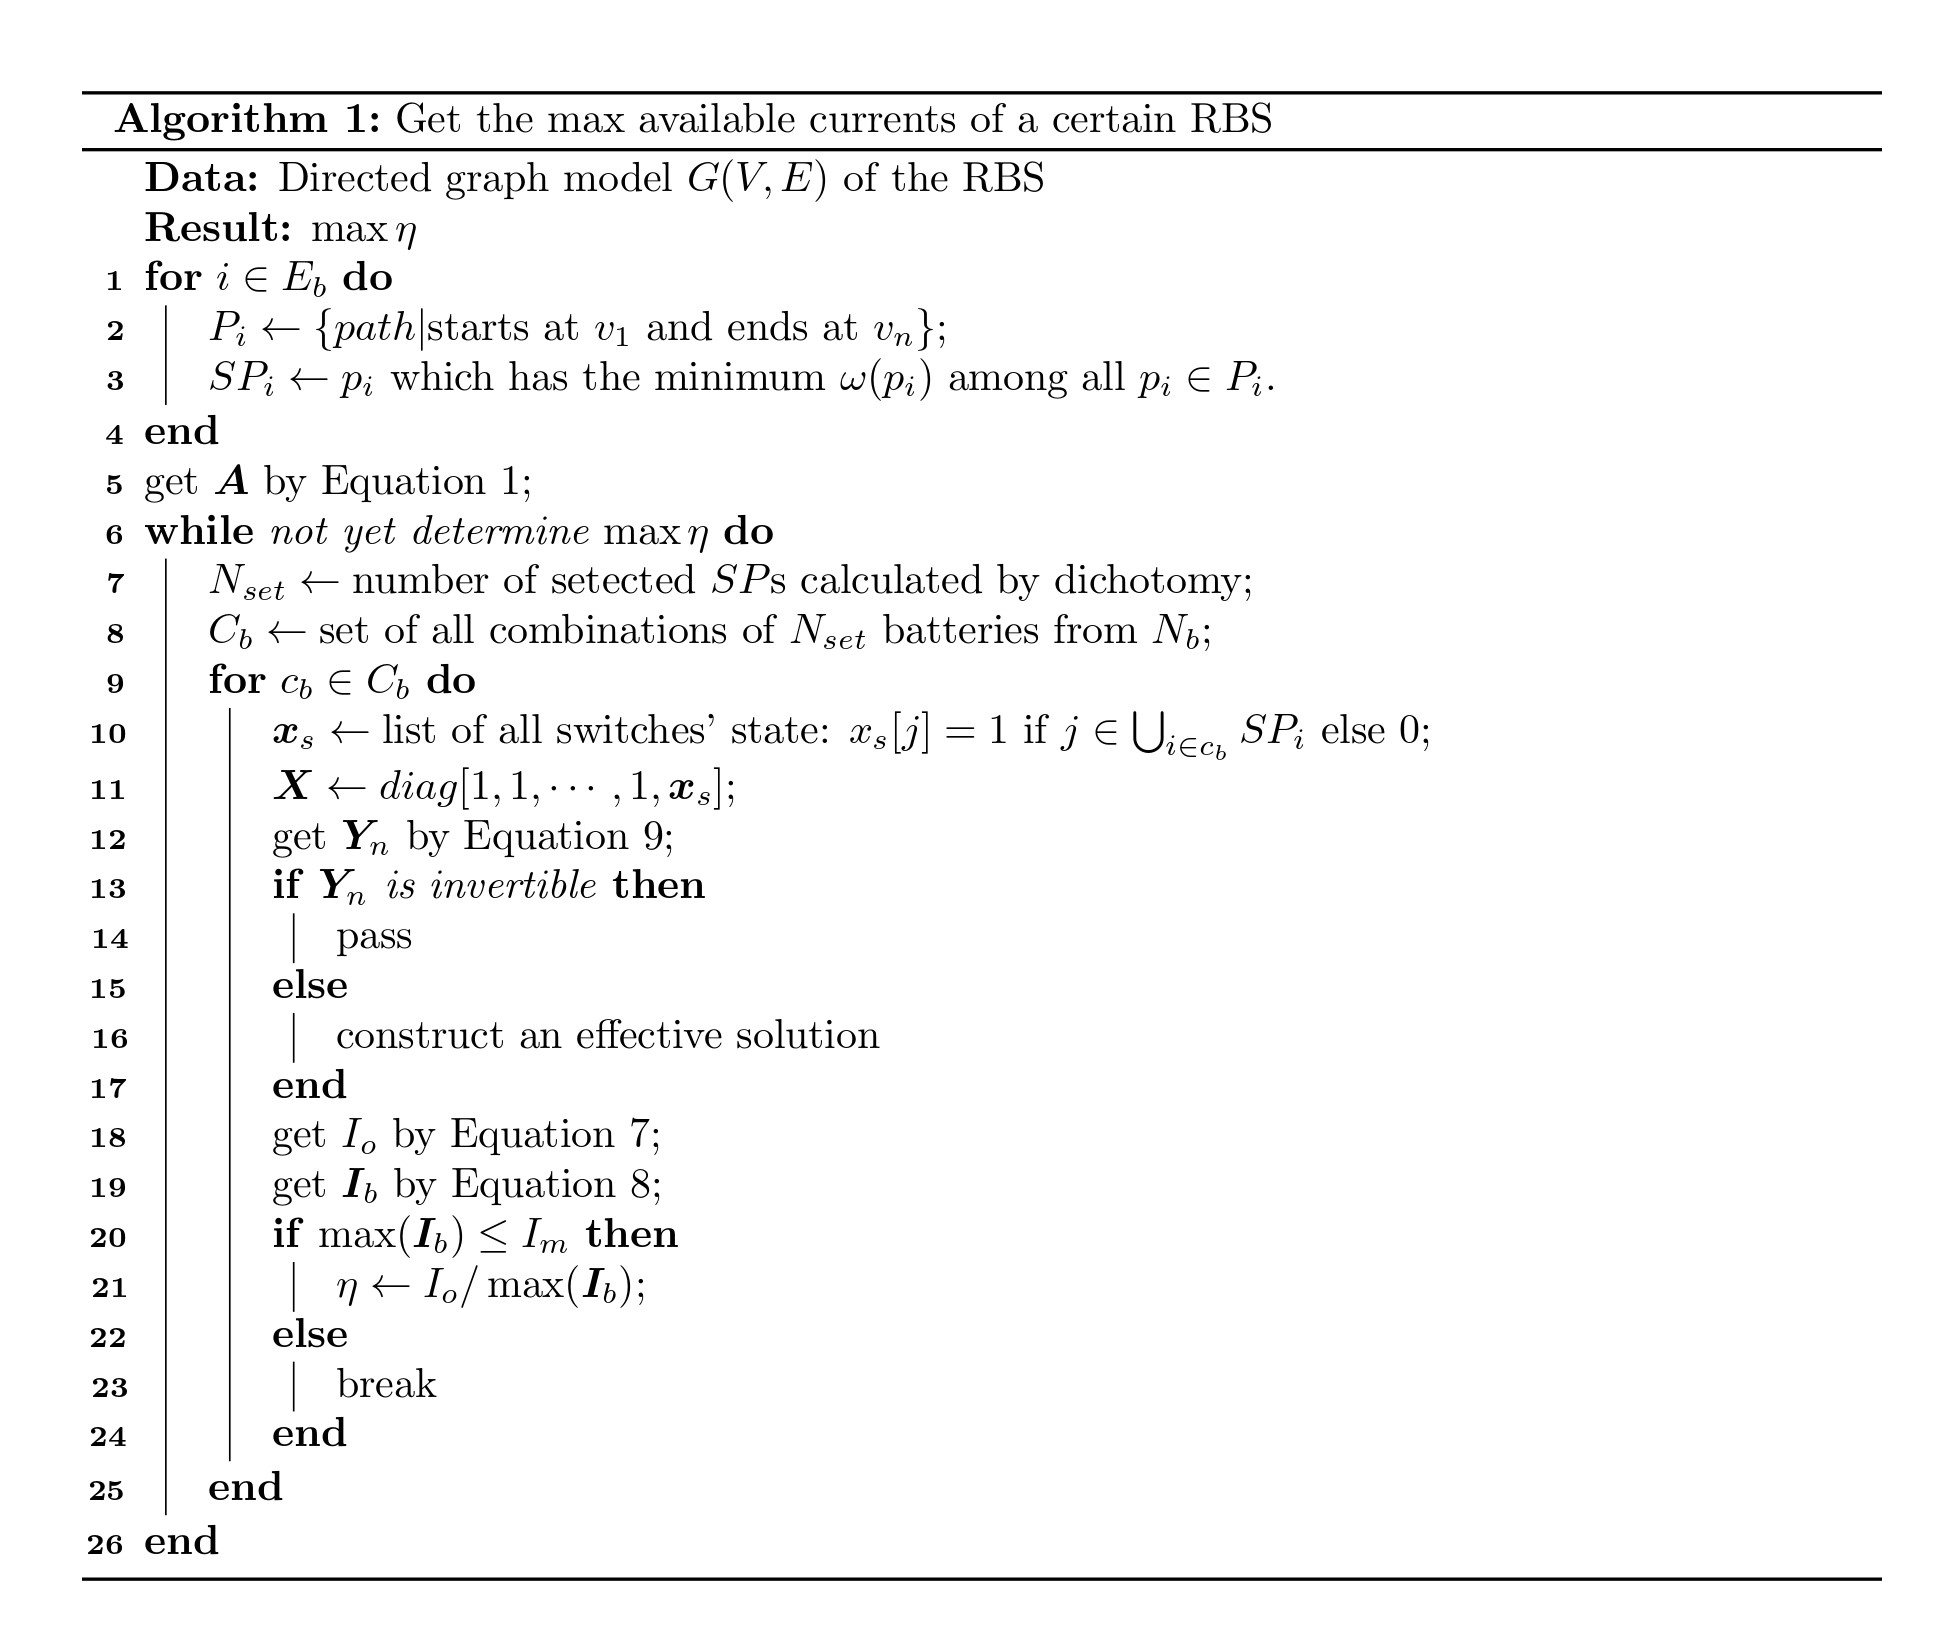
\includegraphics[width=\textwidth]{algorithm.jpg}
% \end{figure}


\section*{Acknowledgments}

\subsection*{Author Contributions} 

B. Xu conceived the main idea, formulated the overarching research goals and aims, designed the algorithm, and reviewed and revised the manuscript.
G. Hua developed and analyzed the model, implemented the code and supporting algorithms, and wrote the initial draft.
C. Qian provided critical review, commentary, and revisions.
Q. Xia contributed to shaping the research, analysis, and manuscript.
B. Sun conducted the research and investigation process.
Y. Ren secured the funding and supervised the project.
Z. Wang verified the results and provided necessary resources.

\subsection*{Funding}

This work was supported by the National Natural Science Foundation of China (NSFC, No.52075028).

\subsection*{Conflicts of Interest}

The authors declare that there is no conflict of interest regarding the publication of this article.

\subsection*{Data Availability}

This work does not require any data to be declared or publicly disclosed.

% \bibliographystyle{nejm}
% \bibliography{sst_main}

\printbibliography

\end{document}
